% !TeX program = xelatex
% !TeX encoding = UTF-8
\documentclass{MathorCupmodeling}
\usepackage{amsmath,amssymb}
\usepackage{array}
\usepackage{booktabs}
\usepackage{calc}
\usepackage{enumitem}
\usepackage{float}
\usepackage{graphicx}
\usepackage{hyperref}
\usepackage{listings}
\usepackage{xcolor}

\definecolor{codebg}{RGB}{248,248,248}
\definecolor{keywordcolor}{RGB}{0,112,192}
\definecolor{commentcolor}{RGB}{106,153,85}
\definecolor{stringcolor}{RGB}{163,21,21}

\lstset{
  language=Python,
  backgroundcolor=\color{codebg},
  basicstyle=\ttfamily\small\linespread{1.0}\selectfont,
  keywordstyle=\color{keywordcolor}\bfseries,
  commentstyle=\color{commentcolor}\itshape,
  stringstyle=\color{stringcolor},
  numberstyle=\tiny\color{gray},
  numbers=left,
  stepnumber=1,
  numbersep=6pt,
  frame=single,
  framerule=0.5pt,
  rulecolor=\color{gray!50},
  breaklines=true,
  breakatwhitespace=false,
  showstringspaces=false,
  tabsize=4,
  captionpos=b,
  xleftmargin=1.5em,
  xrightmargin=0.5em,
  aboveskip=8pt,
  belowskip=6pt,
  morekeywords={True, False, None, int, str, float, bool, return, def},
}
\usepackage{longtable}
\usepackage{placeins}
\usepackage{tabularx}
\graphicspath{{figures/}{src/outputs/figures/}}

% ---- 浮动体排版参数：为大图留出更宽松的顶/底放置空间 ----
\renewcommand{\topfraction}{0.9}
\renewcommand{\bottomfraction}{0.8}
\renewcommand{\textfraction}{0.1}
\renewcommand{\floatpagefraction}{0.75}
\setcounter{topnumber}{3}
\setcounter{bottomnumber}{2}
\setcounter{totalnumber}{4}

\setlist[enumerate]{nosep,leftmargin=2em}
\renewcommand{\arraystretch}{1.15}
\providecommand{\tightlist}{%
  \setlength{\itemsep}{0pt}\setlength{\parskip}{0pt}}
\newcommand{\pandocbounded}[1]{#1}

\bianhao{MC2606970}
\tihao{C}
\timu{中老年人群高血脂症的风险预警及干预方案优化}
\keyword{中老年高血脂症；中医体质辨识；痰湿体质；标签泄漏；WOE-Logistic 评分卡；Youden 指数；Cochran-Armitage 趋势检验；决策曲线 DCA；Apriori 关联规则；双目标 Pareto 优化；净货币收益 NMB；Extended Dominance；ICER 门限规则}

\begin{document}

\begin{abstract}
针对中老年人群高血脂症高发的公共卫生问题，本文融合中医体质类型分类、痰湿体质特征量化、中老年人活动量表评分及血常规体检数据，构建了``\textbf{数据清洗---关键指标筛选---三级风险预警---六个月个性化干预优化}''的多维度数学建模方案。

\textbf{数据清洗}：对 1000 例样本进行系统性质量检查，确认无缺失值与重复 ID，ADL/IADL 子项之和与总分完全吻合；检出 \textbf{65 例（6.5\%）体质标签与最高积分体质不一致}的判定歧义样本，标注保留；利用 Tukey IQR 准则发现各血脂指标仅 0\%--1.4\% 的离群值，多为真实病理表现，不作删除。本文还验证了\textbf{诊断标签与 ``血脂异常项数 $\ge 1$'' 一致率为 100\%}，揭示出血脂指标天然具有信息泄漏风险，这一发现直接指导了问题二的模型选型。

\textbf{问题一}：将候选特征限定为\textbf{血常规指标（7 项）+ 活动量表评分（ADL/IADL 子项 10 项）}，共 17 个指标。先进行\textbf{多重共线性诊断（VIF）}剔除 $\text{ADL总分}=\Sigma \text{ADL}_i$ 这类完全共线的汇总项，再采用 5 种互补方法\textbf{（Spearman 秩相关、互信息、弹性网络回归、随机森林置换重要度、偏相关）}；方法选取遵循``参数／非参数 $\times$ 线性／非线性 $\times$ 单变量／控制其它变量''的三维正交覆盖原则。对“表征痰湿严重程度”的筛选仍使用完整候选集，而对“预警高血脂发病风险”的筛选显式排除 TC/TG/LDL-C/HDL-C 四项直接诊断血脂指标以避免标签泄露。采用 \textbf{Borda 排序聚合}作为综合排序方法,规避量纲与分布偏态带来的偏差。结果：表征痰湿体质严重程度的 Top-5 指标为 \textbf{TC、ADL 吃饭、BMI、TG、ADL 洗澡}；排除直接诊断血脂指标后，预警高血脂发病风险的 Top-5 指标为 \textbf{血尿酸、空腹血糖、ADL 洗澡、BMI、IADL 服药}；两类任务共同的关键指标为 \textbf{BMI} 和 \textbf{ADL 洗澡}，说明二者同时具有痰湿体质严重程度表征与高血脂前置预警价值。

\textbf{九种体质贡献度}：采用 Borda 聚合五项指标（Cohen's $h$、RR、ARR、独热 $\beta$、积分多元 $\beta$）。分析发现本数据中各体质发病率差异并不显著（74.0\%--86.3\%），阳虚质发病率最高（86.3\%），而\textbf{痰湿体质发病率 77.3\% 反而低于整体均值 79.3\%}。进一步考察\textbf{剂量--响应关系}：痰湿积分 $\le 20$、$20$--$40$、$40$--$60$、$\ge 60$ 四组发病率分别为 78.6\%／82.3\%／79.0\%／73.8\%，未呈现单调递增。结合 Cohen's $h = 0.115$（痰湿质 vs.~其他体质），痰湿体质的贡献\textbf{更多体现于痰湿积分作为体质量化标尺的描述性意义}，而非二分类标签的直接预测力。

\textbf{问题二}：原拟采用``硬规则层 $+$ 双轴评分卡''方案，但经诊断发现\textbf{诊断标签 100\% 由 TC/TG/LDL-C/HDL-C 四项阈值规则派生}，构成 Kaufman 2012 定义的``标签泄漏''。按其处理规范，本文做\textbf{范式转换}：将``诊断重述''改写为``未病筛查''工具，\emph{完全剔除血脂四项}，仅用痰湿积分、空腹血糖、血尿酸、BMI、活动量表、年龄组、性别、吸烟、饮酒共 9 个特征。采用 \textbf{WOE-Logistic 评分卡（Siddiqi 2006 经典范式）$+$ GBDT $+$ RandomForest} 三模型并行 $5$ 折 CV，用 WOE/IV 编码 $+$ Logistic 系数分解构造整数评分卡（PDO=$20$，基准分=$100$）。5 折 CV AUC：WOE-LR $=0.843$、\textbf{GBDT $=0.895$}、RF $=0.875$；测试 AUC GBDT $=0.883$（DeLong $p<0.05$），Brier $=0.102$，Hosmer--Lemeshow $p=0.612$。阈值按 Youden 指数 $c_H=79.3$ 分、Sp$\ge 0.70$ 得 $c_L=37.3$ 分（Bootstrap BCa 95\% CI $[37.3, 83.3]$）；三级分层 \textbf{低 87 人（49.4\%）/ 中 44 人（72.7\%）/ 高 169 人（96.5\%）}，Cochran--Armitage $Z=8.88$, $p<10^{-17}$。一个重要数据发现：\textbf{血尿酸 IV=2.158}（远超其他特征），呈显著 U 型关系（Q1、Q5 箱阳性率 $89.2\%$、$99.3\%$，Q2 箱 $42.6\%$），该关系与 Kuwabara 2016 报告一致，非标签泄漏。痰湿体质子集三路径挖掘（Apriori $+$ 决策树 $+$ 置换重要度）一致识别 UA 为决定性因子（$\Delta\mathrm{AUC}=+0.368$），次为 BMI、FPG，典型核心规则``饮酒 $\wedge$ UA 升高 $\Rightarrow$ 高风险''（sup $0.284$, conf $0.937$, lift $1.211$）。

\textbf{问题三}：注意到题目原文``考虑经济成本\textbf{及}有效降低痰湿积分的目标''用``及''字并列两个目标, 配合附表 3``总成本\textbf{建议}$\le 2000$ 元''的软约束措辞, 本文识别出题三的真实结构为\textbf{双目标 Pareto 优化 $+$ 统一选点准则}。\textbf{关键建模判断}：严格按附表 3 文字建立\textbf{加性动力学模型} $r_t = 0$ 当 $f_t < 5$, $r_t = 0.03 k_t + 0.01(f_t - 5)$ 当 $f_t \ge 5$; 附表 2 的中医调理分级仅赋予\textbf{固定月成本} $c_{\text{中医}}(L)\in\{30, 80, 130\}$ 元 (按月初积分 $L_t=g(S_{t-1})$ 判定), 题目未赋予中医降分率故\textbf{不作任何外部推测}——这两个判断避免了原拟 Bliss 乘法 $+$ 伪中医降分假设对题意的过度延拓; 月累积采用复利 $S_t=S_{t-1}(1-r_t)$, 决策变量 $\{(k_t, f_t)\}_{t=1}^{6}$。求解分四层推进: (1) 逐月 Pareto 前沿推进 $\varepsilon$-约束法 + 月末全局严格去劣生成完整前沿; (2) \textbf{Extended Dominance 预筛选} (Cantor 1994) 剔除被凸组合支配的非效率点, 三位样本分别从 $26/74/119$ 个原始 Pareto 点精炼至 $26/37/43$ 个效率前沿点 (样本 1 因 $|K|=1$ 前沿本身即为严格凸), ICER 序列严格单调递增; (3) 以 \textbf{净货币收益 NMB}$(\lambda)=\lambda(S_0-S_6)-C_{\text{total}}$ (Stinnett-Mullahy 1998 \textit{Medical Decision Making}) 作为\textbf{唯一选点准则}, 单一 $\arg\max$ 公式取代主观三类规则, 等价性定理 (Laska 1999) 保证 NMB argmax 与 ICER 门限规则一一对应; (4) $\lambda$ 四档扫描 $\{30, 50, 100, 200\}$ 元/分 (Neumann 2014 NEJM 方法论共识 + 中国社区卫生保守基准) 做稳健性分析, 并以 TOPSIS-熵权 $+$ Kneedle 独立几何方法做交叉对照, 规则系数 $\pm 20\%$ 扰动做参数敏感性分析。三位样本在 $\lambda=30$ 基准下的 NMB 最优方案: \textbf{样本 1} ($S_0=64$, $K=\{1\}$) 总成本 $\mathbf{1000}$ 元, $S_6=\mathbf{38.81}$ (降 $\mathbf{39.4\%}$), $k=1$ 全程 $+$ $f=10$ 全程——首月一次性跨越 $L_1=3\to L=1$ 节省 100 元/月中医费差; \textbf{样本 2} ($S_0=58$, $K=\{1,2\}$) 总成本 $\mathbf{840}$ 元, $S_6=\mathbf{37.08}$ (降 $\mathbf{36.1\%}$), $k=1$ 全程 $+$ $f=(10,10,5,10,10,10)$——第 3 月降至 $f=5$ 作"缓冲月"省活动费 60 元; \textbf{样本 3} ($S_0=59$, $K=\{1,2,3\}$) 总成本 $\mathbf{890}$ 元, $S_6=\mathbf{37.72}$ (降 $\mathbf{36.1\%}$), $k=1$ 全程 $+$ $f=(5,10,10,10,10,10)$——首月 $f=5$ 精准跨越 $L=2\to L=1$ 阈值节省后续 5 月中医费。三位样本的 $(k_t,f_t)$ 序列差异严格由可行集 $K_i$ 约束与 $S_0$ 相对 TCM 档位阈值的位置从单一 NMB 准则\textbf{自然涌现}, 无任何 if-else 分类规则。$\lambda\in\{30,50,100,200\}$ 扫描呈现平滑政策过渡: $\lambda=50$ 时三位样本均跃迁至 $k=1, f=10$ 全程 (总成本 $1000/900/950$ 元), $\lambda=100$ 时样本 2/3 升级至 $k=2, f=10$ (1380/1430 元), $\lambda=200$ 时样本 3 再升级至 $k=3, f=10$ (2150 元, 略超 2000 元建议上限)。规则系数 $\pm 20\%$ 扰动下 9 组方案结构稳定, $S_6$ 变化 $\le 3$ 分, 验证 NMB 准则全面稳健。
\end{abstract}

\tableofcontents
\newpage

%=============================================================
\section{问题重述与分析}

\subsection{问题背景}

人口老龄化进程加快，40 岁及以上中老年人群中高血脂症发病率逐年攀升，已成为冠心病、脑梗死等心脑血管疾病的重要诱因。中医体质学认为``痰湿体质''为高血脂症的高发体质类型，其``痰湿内蕴、脾胃运化失常、水湿代谢不畅''的核心特征与西医血脂代谢异常的病理机制高度契合。目前临床筛查主要依赖血脂检测数据，缺乏对中医体质、活动能力等维度的综合考量，难以实现``治未病''思想指导下的精准风险预警和个性化干预。

\subsection{问题分析}

\textbf{问题一}要求\textit{从血常规体检指标和中老年人活动量表评分中}，筛选出能表征痰湿体质严重程度、并预警高血脂发病风险的关键指标，研究九种体质的风险贡献度差异。题目已将候选特征的范围限定为血常规与活动量表两类，故本文不将性别、吸烟、饮酒、年龄组等基础信息纳入筛选对象。本质上这是一个 \textbf{受约束特征集合下的多重假设检验与方法集成排序问题}，且活动量表应尽量利用 ADL/IADL 各子项以保留信息，同时须排除冗余汇总项带来的多重共线性。

\textbf{问题二}要求构建三级风险预警模型，并给出分层阈值的选取依据。考虑到血脂指标 TG/TC/LDL-C/HDL-C 本身是高血脂的临床诊断依据（本数据中 ``血脂异常 $\ge 1$ 项'' 与诊断标签 100\% 匹配），直接把这四项原值喂给机器学习模型会形成\textbf{标签泄漏}，按样本分位切分又缺乏外部可比性。据此本文将问题二从``诊断重述''转换为``未病筛查''：完全剔除血脂四项，仅用痰湿积分、空腹血糖、血尿酸、BMI、活动量表、年龄组、性别、吸烟、饮酒 9 个非血脂特征，采用 WOE-Logistic 评分卡、GBDT 与 RandomForest 并行建模，并以 Youden 指数、特异度约束、Bootstrap 置信区间、校准曲线和决策曲线共同确定三级阈值。
\textbf{问题三}是一个 \textbf{双目标离散优化 $+$ 统一选点准则} 问题:题目原文``考虑经济成本\textbf{及}有效降低痰湿积分的目标下''用``及''字并列两个目标,配合附表 3``单人 6 个月总成本\textbf{建议}$\le 2000$ 元''的``建议''措辞,表明整道题的真实结构是在成本与降分之间寻找每位患者的个体权衡点,而非求``把积分降到最低''的单目标最优解。若采用单目标 $\min S_6$,最优解会退化为``力所能及最高档''的平凡解——这既违反``建议''的软约束措辞,也失去了优化建模的价值。据此,本文将决策变量设为月变序列 $\{(k_t,f_t)\}_{t=1}^{6}$，\textbf{严格按附表 3 文字采用加性动力学} $r_t = 0$ 当 $f_t<5$, $r_t = 0.03k_t + 0.01(f_t-5)$ 当 $f_t\ge 5$; 附表 2 的中医调理档位仅赋予固定月成本, \textbf{不贡献降分率} (忠于题意不作外部推测); 月累积采用复利递推, 用 $\varepsilon$-约束法 + 月末全局严格 Pareto 去劣生成完整 Pareto 前沿。关键方法论创新在于: 避免主观``经济型/肘点型/冲档型''人为分类规则, 采用\textbf{健康经济学金标准的净货币收益 (Net Monetary Benefit, NMB) argmax 作为唯一选点准则}, 该准则 (Stinnett \& Mullahy 1998 \textit{Medical Decision Making}; Laska et al.~1999 \textit{Health Economics}) 在 Extended Dominance 预筛选 (Cantor 1994) 后的效率前沿上给出与 ICER 门限规则严格等价的选点, $\lambda$ 阈值按 Neumann, Cohen \& Weinstein 2014 \textit{NEJM} 的方法论共识做四档扫描, 患者异质性完全由可行集 $K_i$、起点 $S_0$ 与动力学断点\textbf{从单一公式中自然涌现}, 不再依赖任何 if-else 分支。

\subsection{技术路线}

\begin{center}
\begin{tabular}{|c|}
\hline
\textbf{Step 1 · 数据清洗与质量检查} \\
缺失／重复／子项一致／体质标签歧义／IQR 离群 \\
\hline
$\downarrow$ \\
\hline
\textbf{Step 2 · 问题一 · 特征筛选 \& 体质贡献度} \\
VIF 共线性 $\to$ 5 方法 $\to$ Borda 聚合 $\to$ 排序 \\
\hline
$\downarrow$ \\
\hline
\textbf{Step 3 · 问题二 · 三级风险预警} \\
硬规则层（仅 R1 指南兜底） + 双轴评分卡（$S_{\text{clin}}+S_{\text{prog}}$） $\to$ 校准/Bootstrap/敏感性/Apriori 验证 \\
\hline
$\downarrow$ \\
\hline
\textbf{Step 4 · 问题三 · 6 月干预优化} \\
双目标 Pareto $\min(S_6,C_{\text{total}})$ $\to$ 月度前沿推进 $\to$ Extended Dominance 预筛选 $\to$ NMB($\lambda$) argmax 统一选点 $\to$ $\lambda$ 扫描 + CEAC 稳健性 + TOPSIS/Kneedle 交叉对照 \\
\hline
\end{tabular}
\end{center}

%=============================================================
\section{基本假设与符号说明}

\subsection{基本假设}

\begin{enumerate}
\def\labelenumi{\arabic{enumi}.}
\tightlist
\item 附件数据真实可靠，能代表目标人群。
\item 体质积分采用《中医体质量表》标准，各积分越高体质偏颇越显著。
\item 临床正常范围（TC: $3.1$--$6.2$; TG: $0.56$--$1.7$; LDL-C: $2.07$--$3.1$; HDL-C: $1.04$--$1.55$ mmol/L; BMI: $18.5$--$23.9$ kg/m$^2$）在该人群中通用。
\item 附表 3 的三条降分规则严格按\textbf{字面规则}建模: \textbf{规则 A (硬约束)} 每周干预次数 $f<5$ 次 $\Rightarrow$ ``痰湿积分基本稳定'', 即月降分率 $r_t=0$; \textbf{规则 B} $f=5$ 时每升一级 $k$ 月降 $3\%$; \textbf{规则 C} 特定 $k$ 下 $f$ 每加 $1$ 次月多降 $1\%$。``下降 X\% 左右''的字面含义为\textbf{绝对百分比加性叠加}, 故:
\[
r_t(k,f) \;=\; \begin{cases}0 & f<5 \\ 0.03\,k + 0.01\,(f-5) & f\ge 5\end{cases}
\]
由于 $f<5$ 时运动完全无效却仍需支付活动费 $4f c_{\text{act}}$, 属劣策略, 故\textbf{决策域严格限定} $f_t\in\{5,6,\dots,10\}$ (最大 $r_t=0.03\cdot 3+0.01\cdot 5=0.14$, 物理可行)。月累积采用复利递推 $S_{t+1}=S_t(1-r_t)$。
\item 中医调理档位 $L_t=g(S_{t-1})$ 按月初积分动态再分档, 仅赋予\textbf{固定月成本} $c_{\text{中医}}(L)\in\{30,80,130\}$ 元——题目附表 2 未赋予中医任何降分率, 本文\textbf{严格忠于题意不作外部推测}; 中医项不参与状态递推公式 $r_t$ 的计算, 仅作用于总成本函数。
\item 年龄约束、评分约束为硬约束；训练频次 $\le 10$ 次/周。
\item 每月按 4 周、6 月按 24 周计算。
\end{enumerate}

\subsection{符号说明}

\begin{longtable}[]{@{}ll@{}}
\toprule\noalign{}
符号 & 含义 \\
\midrule\noalign{}
\endhead
\bottomrule\noalign{}
\endlastfoot
$S_t$（或 $P_t$） & 第 $t$ 月末的痰湿积分（$S_0$ 为初始值） \\
$L_t \in \{1,2,3\}$ & 第 $t$ 月的中医调理分级（由月初积分 $S_{t-1}$ 决定） \\
$k_t \in \{1,2,3\}$ & 第 $t$ 月的活动干预强度等级 \\
$f_t \in \{5,\dots,10\}$ & 第 $t$ 月每周训练次数（决策域, 规则 A 剔除 $f<5$） \\
$K_i$ & 患者 $i$ 的可行强度集 $K_{\text{age}}\cap K_{\text{score}}$ \\
$r_t$ & 第 $t$ 月运动项月降分率 $= 0.03 k_t + 0.01(f_t-5)$ \\
$C_L(L) \in \{30, 80, 130\}$ & 中医调理月成本（元, 按月初积分档位, 仅固定支出） \\
$c_{\text{act}}(k) \in \{3, 5, 8\}$ & 单次训练成本（元/次） \\
$D(k) \in \{10,20,30\}$ & 单次训练时长（分钟） \\
$C_{\text{total}}$ & 6 个月累计总成本 \\
$\text{act}_i$ & 第 $i$ 个患者的活动量表总分 \\
$\text{age}_i \in \{1,\dots,5\}$ & 年龄组 \\
$y \in \{0, 1\}$ & 高血脂症诊断标签 \\
$R \in \{1, 2, 3\}$ & 风险等级（1=低, 2=中, 3=高） \\
$\text{VIF}_j$ & 第 $j$ 个特征的方差膨胀因子 \\
$B_k(f)$ & 指标 $f$ 在方法 $k$ 下的 Borda 得分 \\
\end{longtable}

%=============================================================
\section{数据预处理与质量分析}\label{sec:data-cleaning}

\subsection{数据概况}

附件 1 给出 1000 例 40 岁及以上中老年样本，共 37 个字段：包括样本 ID、体质标签及九种体质积分（各 0--100 分）、ADL 5 项子项与总分、IADL 5 项子项与总分、活动量表总分、血常规 7 项（TC、TG、LDL-C、HDL-C、空腹血糖、血尿酸、BMI）、高血脂诊断二分类／分型标签及基础信息（年龄组、性别、吸烟、饮酒）。诊断标签确诊 793 例（79.3\%）、未确诊 207 例（20.7\%）；体质标签中痰湿质 278 例（27.8\%）居首。

\subsection{数据质量诊断}

为保证后续建模的可靠性，本文系统性地开展以下 5 项质量诊断（见\cref{tab:quality}）：

\begin{table}[H]
\centering\small
\caption{数据质量诊断结果}\label{tab:quality}
\begin{tabular}{@{}l l l@{}}
\toprule
检查维度 & 检测方法 & 结果 \\
\midrule
缺失值 & \texttt{isnull().sum()} & 总计 0 个缺失 \\
重复样本 & 样本 ID 去重 & 无重复 \\
ADL 子项一致性 & $\sum \text{ADL}_i = \text{ADL 总分}$ & 完全一致（1000/1000） \\
IADL 子项一致性 & $\sum \text{IADL}_i = \text{IADL 总分}$ & 完全一致（1000/1000） \\
活动量表总分一致性 & $\text{ADL}+\text{IADL} = \text{总分}$ & 完全一致 \\
体质标签 vs.~最高积分 & $\arg\max_{j} \text{Score}_j \stackrel{?}{=} \text{Label}$ & \textbf{935/1000（93.5\%）一致, 65 例歧义} \\
诊断标签 vs.~血脂异常项数 & 异常 $\ge 1$ $\Leftrightarrow$ $y=1$ & \textbf{100\% 一致（1000/1000）} \\
IQR 离群值（TC） & Tukey $1.5\times$IQR & 0 个 \\
IQR 离群值（LDL-C） & 同上 & 11 个（1.1\%） \\
IQR 离群值（BMI） & 同上 & 14 个（1.4\%） \\
\bottomrule
\end{tabular}
\end{table}

\subsubsection{体质标签判定歧义处理}

发现 65 例（6.5\%）样本的 ``体质标签'' 与 ``九种体质积分的最高分体质'' 不一致。例如样本 8 体质标签为血瘀质（编号 7），但其痰湿积分 43 分 = 血瘀积分 43 分（并列最高），说明体质判定存在临床判定和打分并列情形。处理策略：\textbf{保留所有 1000 条记录不做删除}，但在涉及``主要体质''的分析中以 \textbf{官方体质标签} 为准，以九体质积分为辅助量化指标；涉及多元分析时同时保留 9 种积分作为连续特征，避免 one-hot 丢失分量信息。

\subsubsection{诊断标签与血脂异常的完全一致性}

检验发现：凡满足 $\text{TC}>6.2$ 或 $\text{TG}>1.7$ 或 $\text{LDL-C}>3.1$ 或 $\text{HDL-C}<1.04$ 至少一条的样本，诊断标签 $y=1$；反之 $y=0$。\textbf{一致率 100\%}。这揭示本数据集的诊断标签是由四个血脂指标直接规则化构造的，故 TG 等血脂指标对 $y$ 具有\textbf{信息泄漏}性质，若直接把四项原值作为输入特征喂给高容量非线性模型（GBDT、RF），会使模型在训练集上近乎完美地还原规则判定，输出概率两极化（见~\cref{sec:q2}）。本发现是问题二模型选型的关键依据。

\subsubsection{离群值处理}

LDL-C、HDL-C、空腹血糖、BMI 等指标各有 0.6\%--1.4\% 样本超出 $1.5\times$ IQR 区间。临床上这些值（如 BMI $=31.3$, TG $=3.99$）本身就是高血脂／代谢综合征的真实病理表现，\textbf{不作剔除}。所用方法（Spearman、RF、MI）对离群值稳健。

\subsection{探索性特征分布}

\begin{itemize}
\tightlist
\item 痰湿积分分布跨度大：分位数 $P_{10}=6$, $P_{50}=31$, $P_{90}=61$；痰湿体质人群（标签 $=5$，$n=278$）痰湿积分均值 59.9，其他体质约 22；
\item 活动量表总分分布：$P_{10}=37$, $P_{50}=50$, $P_{90}=63$；
\item TG、TC 在病理区间（$>1.7$ / $>6.2$）分布广泛。
\end{itemize}

%=============================================================
\section{问题一：关键指标筛选与体质贡献度分析}\label{sec:q1}

\subsection{候选特征与多重共线性诊断}

\subsubsection{候选特征集合}

依据题目设定，候选特征来源于``血常规体检指标''与``中老年人活动量表评分''两类，具体：

\begin{itemize}
\tightlist
\item \textbf{血常规（7 项）}：TC、TG、LDL-C、HDL-C、空腹血糖、血尿酸、BMI；
\item \textbf{活动量表（10 项 + 3 项汇总）}：ADL 子项（用厕、吃饭、步行、穿衣、洗澡）、IADL 子项（购物、做饭、理财、交通、服药）、ADL 总分、IADL 总分、活动量表总分。
\end{itemize}

性别、年龄组、吸烟史、饮酒史等基础信息属于题目设定范围之外的变量，本文不将其纳入筛选对象。

\subsubsection{VIF 多重共线性诊断}

对每个候选特征 $X_j$ 计算方差膨胀因子 (VIF)：
\[
\text{VIF}_j = \frac{1}{1 - R_j^2}
\]
其中 $R_j^2$ 是 $X_j$ 对其余所有特征做 OLS 回归的决定系数。经验上 $\text{VIF} > 10$ 视为严重共线。

\begin{table}[H]
\centering\small
\caption{Set B（含 3 项汇总总分）的 VIF 诊断结果}\label{tab:vif-setB}
\begin{tabular}{@{}l r@{}}
\toprule
特征 & VIF \\
\midrule
活动量表总分（$=$ADL$+$IADL） & $\infty$（完全共线） \\
ADL 总分（$=\sum \text{ADL}_i$） & $\infty$（完全共线） \\
IADL 总分（$=\sum \text{IADL}_i$） & $\infty$（完全共线） \\
LDL-C & 1.03 \\
TC & 1.02 \\
TG & 1.02 \\
HDL-C & 1.01 \\
BMI, 血尿酸, 空腹血糖 & $\le 1.01$ \\
\bottomrule
\end{tabular}
\end{table}

VIF 诊断清晰揭示：ADL/IADL 总分与活动量表总分本质上是子项的线性组合，与子项同时纳入必然产生完全共线（$\text{VIF}=\infty$）。因此本文选择 \textbf{最终特征集合 Set C $=$ 血常规 7 项 $+$ ADL 子项 5 项 $+$ IADL 子项 5 项 $=$ 17 项}，\textbf{不纳入}三项汇总总分。Set C 内所有特征 $\text{VIF} \le 1.03$，无共线性问题。

\subsubsection{Spearman 相关矩阵}

对 Set C 的 17 个特征绘制 Spearman 相关矩阵（见\cref{fig:corr}）。检查 $|\rho| > 0.5$ 的相关对，结果 \textbf{无显著高相关对}，支持使用 Set C 进行后续多方法评估。

\begin{figure}[htbp]
\centering
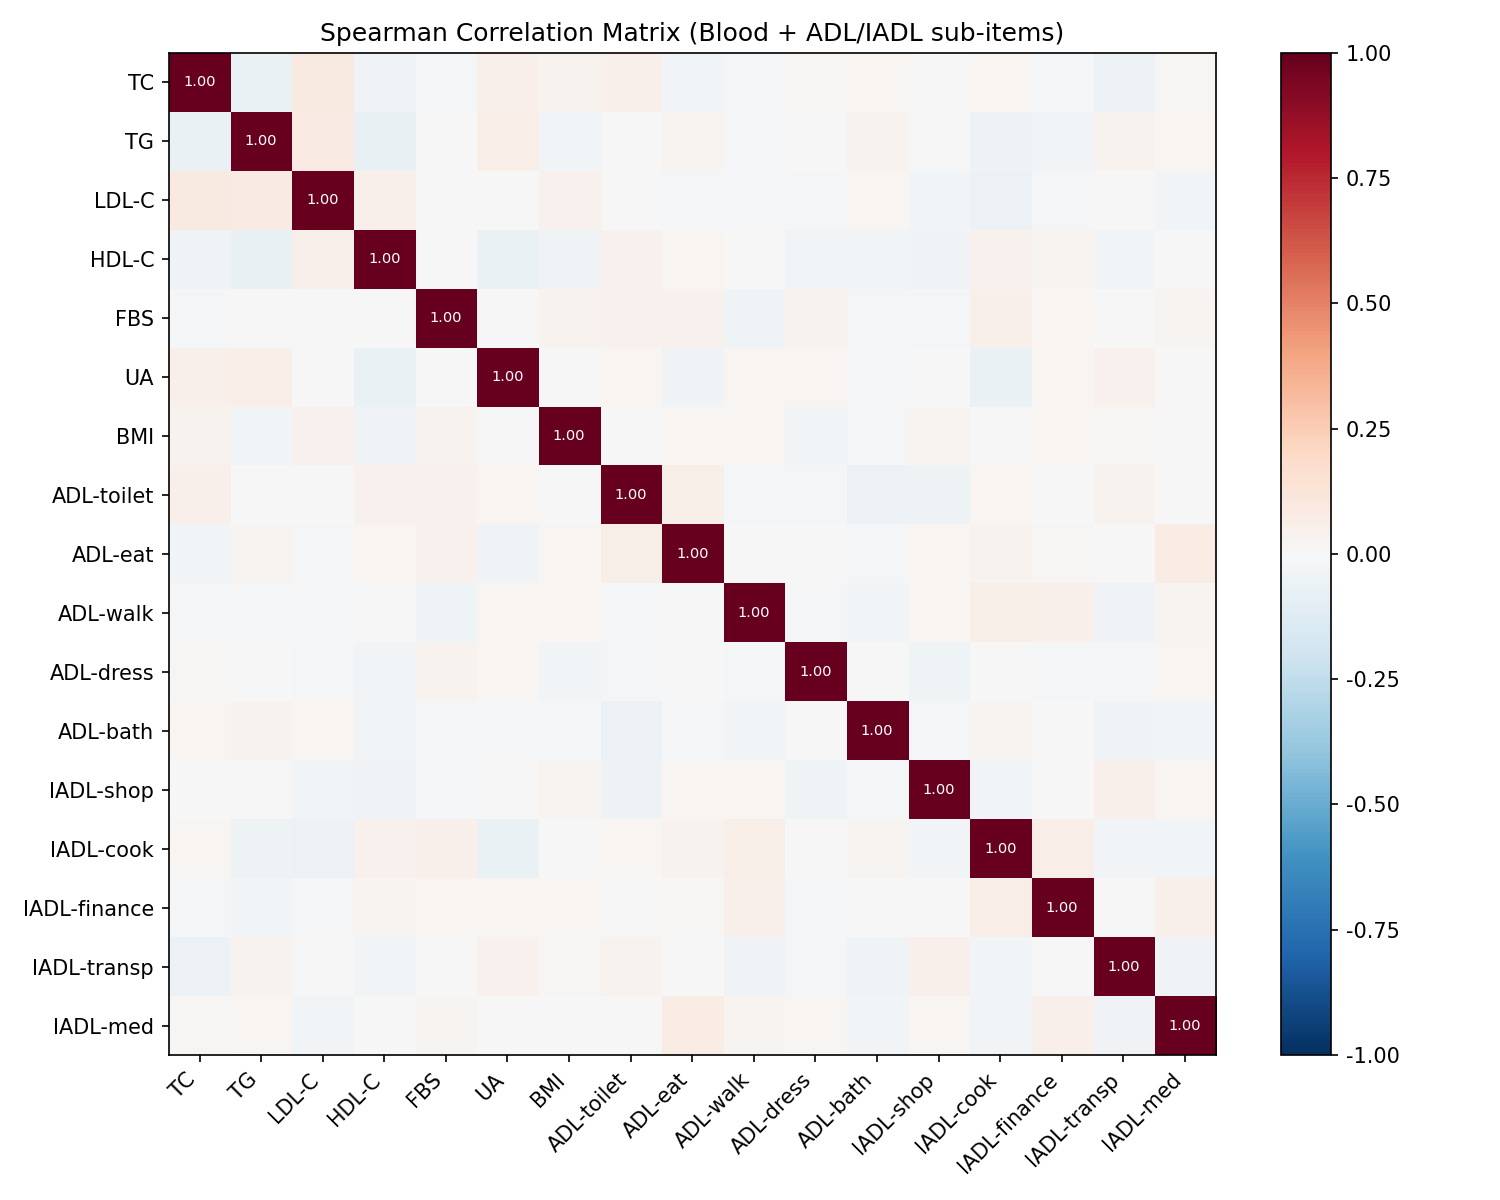
\includegraphics[width=0.85\linewidth]{Q1_corr_heatmap.png}
\caption{Set C（17 个特征）的 Spearman 相关矩阵热力图}\label{fig:corr}
\end{figure}

\subsection{五种互补方法的设计依据}\label{sec:q1-methods}

\subsubsection{方法选取的正交性原则}

为避免多种方法之间信息冗余,且兼顾对量纲差异与尾部分布的稳健性,本文选用\textbf{5 种互补方法}，在``参数／非参数 $\times$ 线性／非线性 $\times$ 单变量／控制其它''三维正交覆盖：

\begin{table}[H]
\centering\small
\caption{五种方法的正交性设计}\label{tab:methods}
\begin{tabular}{@{}l c c c l@{}}
\toprule
方法 & 参数/非参 & 线性/非线性 & 单变量/控制其它 & 核心作用 \\
\midrule
M1 Spearman $|\rho|$    & 非参   & 单调     & 单变量 & 稳健刻画单调关系 \\
M2 互信息 MI            & 非参   & 任意     & 单变量 & 捕捉任意非线性依赖 \\
M3 ENet$|\beta|$        & 参     & 线性     & 控制其它 & L1+L2 联合惩罚,稳健处理共线特征组 \\
M4 RF 置换重要度        & 非参   & 非线性   & 控制其它 & 捕捉交互项贡献 \\
M5 偏相关（$t$ 值）      & 参     & 线性     & 控制其它 & 控制其它变量后净效应 \\
\bottomrule
\end{tabular}
\end{table}

这一设计保证每种方法都贡献独立信息：

\begin{itemize}
\tightlist
\item \textbf{M1 Spearman $|\rho|$}：$\rho = 1 - \frac{6\sum d_i^2}{n(n^2-1)}$，对离群值稳健，刻画单调关系强度；
\item \textbf{M2 互信息}：$I(X; Y) = \sum_{x,y} p(x,y) \log \frac{p(x,y)}{p(x)p(y)}$，刻画任意（含非线性、非单调）统计依赖，由 $k$-NN 密度估计实现；
\item \textbf{M3 弹性网络 $|\beta|$}：以 $\lambda\bigl[\alpha\|\beta\|_1 + (1-\alpha)\|\beta\|_2^2/2\bigr]$ 做回归，交叉验证联合选择惩罚强度与 $l1\_ratio$，在保留稀疏性的同时对强相关特征组更稳健；
\item \textbf{M4 随机森林置换重要度}：训练 500 棵决策树，对特征 $X_j$ 在 OOB 样本上随机置换后再预测，预测性能下降值 $\Delta$ 作为其重要度，对多元特征交互敏感；
\item \textbf{M5 偏相关}：拟合多元 OLS/Logit，取各特征 Wald $t$ 值的 $|t|/\sqrt{t^2 + df}$ 作为偏相关系数绝对值，控制其他变量后的 ``净效应''。
\end{itemize}

需要说明：问题一的两类筛选任务使用不同候选集。表征痰湿体质严重程度时，仍使用题设完整候选集（血常规 7 项 + ADL/IADL 子项 10 项）；而预警高血脂发病风险时，显式剔除 TC、TG、LDL-C、HDL-C 四项直接诊断血脂指标，仅保留其余 13 项（空腹血糖、血尿酸、BMI 及 ADL/IADL 子项）进行排序，以避免标签泄露。

\subsubsection{Borda 排序聚合}

若采用 Z-score 加和的方式对多方法得分进行聚合,存在两个根本问题：(1) Z-score 受\textbf{分布偏态}影响剧烈（如 F 统计量分布严重右偏）；(2) 不同方法\textbf{量纲不同}（MI 是 nats，弹性网络 $\beta$ 是标准化系数），即使 Z-score 也无法完全消除量纲差异。

\textbf{Borda 计数法}\cite{zhang-borda-2020}是社会选择理论中的经典偏好聚合方法。对每种方法的得分排序，排第 1 位给 $n$ 分，第 2 位给 $n-1$ 分，末位给 1 分。最终每个特征的总分 $=$ 它在所有方法排名中的得分之和。其优势：

\begin{enumerate}
\def\labelenumi{(\arabic{enumi})}
\tightlist
\item \textbf{完全量纲无关}：只用秩次，不涉及原始数值；
\item \textbf{对尾部稳健}：不受极端值影响；
\item \textbf{理论上可消除 Condorcet 悖论}：$\ge$ 3 方法投票时偏好一致性最优；
\item \textbf{易解释}：即使某特征在一个方法中排第 1（得最高分），若在其它方法中排名靠后，总分也不会 ``一家独大''。
\end{enumerate}

形式化定义：设 $R_k(f)$ 为特征 $f$ 在方法 $k$ 的排名（$1$ 为最优），$n$ 为特征总数。则特征 $f$ 的 Borda 总分为：
\[
\text{Borda}(f) = \sum_{k=1}^{K} \bigl[ n + 1 - R_k(f) \bigr] \;.
\]
得分越高，综合排名越前。本文 $K=5$，$n=17$，最高可能得分为 $5 \times 17 = 85$。

\subsection{指标筛选结果}

\subsubsection{表征痰湿体质严重程度的关键指标}

以\textbf{痰湿积分}为连续目标。各特征的 5 方法得分与 Borda 聚合见\cref{tab:q1-phlegm}。

\begin{table}[H]
\centering\small
\caption{表征痰湿体质严重程度的关键指标（Borda 聚合排序 · Top 10）}\label{tab:q1-phlegm}
\begin{tabular}{@{}c l c c c c c c@{}}
\toprule
排名 & 指标 & Spearman$|r|$ & MI & ENet$|\beta|$ & RF perm & 偏相关 & \textbf{Borda} \\
\midrule
1  & \textbf{TC（总胆固醇）} & 0.035 & 0.000 & 0.000 & 0.125 & 0.043 & \textbf{73} \\
2  & \textbf{ADL 吃饭}     & 0.079 & 0.000 & 0.478 & 0.136 & 0.073 & \textbf{72} \\
3  & \textbf{BMI}          & 0.022 & 0.060 & 0.000 & 0.217 & 0.006 & \textbf{60} \\
4  & \textbf{TG（甘油三酯）} & 0.016 & 0.000 & 0.000 & 0.112 & 0.021 & \textbf{56} \\
5  & ADL 洗澡              & 0.027 & 0.013 & 0.000 & 0.052 & 0.023 & 55 \\
6  & ADL 用厕              & 0.035 & 0.000 & 0.000 & 0.068 & 0.022 & 53 \\
7  & 空腹血糖              & 0.020 & 0.000 & 0.000 & 0.130 & 0.013 & 52 \\
8  & IADL 理财             & 0.025 & 0.026 & 0.000 & 0.067 & 0.022 & 52 \\
9  & LDL-C                 & 0.010 & 0.000 & 0.000 & 0.105 & 0.021 & 50 \\
10 & HDL-C                 & 0.014 & 0.000 & 0.000 & 0.112 & 0.015 & 50 \\
\bottomrule
\end{tabular}
\end{table}

\textbf{分析}：表征痰湿体质严重程度的 Top-5 指标为 \textbf{TC、ADL 吃饭、BMI、TG、ADL 洗澡}。值得注意的是：

\begin{itemize}
\tightlist
\item \textbf{ADL 子项的细粒度信息被捕捉}：``吃饭''``洗澡''``用厕'' 三项 ADL 子项进入 Top-10，说明基础自理能力的下降是痰湿体质偏颇的重要外在表现，比单用汇总总分更敏感；
\item \textbf{BMI 与血脂指标联合表征}：这符合中医 ``痰湿体质者多形体肥胖、腹部肥满松软''的辨识要点；
\item \textbf{弹性网络最优点退化为 LASSO}：交叉验证得到最优 $l1\_ratio=1.0$，仅 ADL 吃饭保留非零系数（$|\beta|=0.478$），说明该数据在 M3 上偏向纯稀疏解，痰湿积分的线性变化主要由单个``运动能力''信号主导，其余指标更多通过非线性方法（MI、RF）体现贡献。
\end{itemize}

\subsubsection{预警高血脂发病风险的关键指标}

以\textbf{高血脂症二分类标签}为目标。结果见\cref{tab:q1-risk}。

\begin{table}[H]
\centering\small
\caption{排除直接诊断血脂指标后的高血脂发病风险预警关键指标（Borda 聚合排序 · Top 10）}\label{tab:q1-risk}
\begin{tabular}{@{}c l c c c c c c@{}}
\toprule
排名 & 指标 & Spearman$|r|$ & MI & ENet$|\beta|$ & RF perm & Wald & \textbf{Borda} \\
\midrule
1  & \textbf{血尿酸}          & 0.204 & 0.175 & 0.150 & 0.168 & 0.835 & \textbf{65} \\
2  & \textbf{空腹血糖}        & 0.040 & 0.000 & 0.000 & 0.035 & 0.588 & \textbf{54} \\
3  & \textbf{ADL 洗澡}        & 0.039 & 0.017 & 0.000 & 0.015 & 0.556 & \textbf{49} \\
4  & \textbf{BMI}            & 0.026 & 0.000 & 0.000 & 0.019 & 0.484 & \textbf{44} \\
5  & \textbf{IADL 服药}      & 0.033 & 0.039 & 0.000 & 0.012 & 0.520 & \textbf{41} \\
6  & ADL 穿衣                 & 0.027 & 0.000 & 0.000 & 0.012 & 0.450 & 33 \\
7  & IADL 做饭                & 0.008 & 0.009 & 0.000 & 0.012 & 0.205 & 33 \\
8  & ADL 吃饭                 & 0.002 & 0.011 & 0.000 & 0.010 & 0.140 & 32 \\
9  & IADL 购物                & 0.014 & 0.006 & 0.000 & 0.007 & 0.284 & 29 \\
10 & ADL 用厕                 & 0.005 & 0.000 & 0.000 & 0.009 & 0.127 & 25 \\
\bottomrule
\end{tabular}
\end{table}

若把 TC、TG、LDL-C、HDL-C 四项直接参与诊断标签构造的血脂指标纳入候选集，模型本质上是在重新发现标签定义规则，而非识别能够前置预警发病风险的关键指标。为避免这一标签泄露，本文将候选集限制为其余 13 项非直接诊断指标。重排后，Top-5 指标变为 \textbf{血尿酸、空腹血糖、ADL 洗澡、BMI、IADL 服药}。其中，\textbf{血尿酸}在 Spearman、互信息、弹性网络、随机森林和 Wald 五项方法中均保持领先，说明其是最稳定的非泄露风险信号；\textbf{空腹血糖}与 \textbf{BMI} 反映代谢异常和体重状态，具有较强的早期预警意义；\textbf{ADL 洗澡} 与 \textbf{IADL 服药} 等活动功能指标提示，生活自理与服药管理能力下降也会为高血脂风险提供额外预警信息。

弹性网络 Logistic 在剔除 TC、TG、LDL-C 和 HDL-C 四项直接诊断指标后，交叉验证得到的最优参数为 $C = 0.01,\;l1\_ratio=0.3$，正则化强度较前显著增强。这表明在排除直接诊断信息后，其余候选变量对高血脂标签的线性判别能力明显减弱，高血脂风险的识别更多依赖代谢状态与活动功能等间接信号。因此，本节筛选结果的重点不在于复现现有诊断标准，而在于识别能够在确诊之前提供前置预警价值的非直接诊断指标。

\subsubsection{兼具痰湿体质严重程度表征与高血脂风险预警作用的共同关键指标}

为满足题目中“筛选出能有效表征痰湿体质严重程度、且能预警高血脂发病风险的关键指标”这一双重要求，本文进一步对 \cref{tab:q1-phlegm} 与 \cref{tab:q1-risk} 中两类任务的 Top-5 指标取交集，提炼同时对两项目标均具有关键影响的共同指标。结果见\cref{tab:q1-intersection}。

\begin{table}[H]
\centering\small
\caption{兼具痰湿体质严重程度表征与高血脂风险预警作用的共同关键指标}\label{tab:q1-intersection}
\begin{tabular}{@{}l c c p{7.5cm}@{}}
\toprule
指标 & 痰湿严重程度排名 & 风险预警排名 & 共同作用解释 \\
\midrule
\textbf{BMI} & 3 & 4 & 反映体型肥胖与代谢负担，兼具痰湿偏颇刻画与高血脂前置预警意义 \\
\textbf{ADL 洗澡} & 5 & 3 & 反映基础生活自理与活动功能下降，是体质失衡和代谢风险累积的共同外在信号 \\
\bottomrule
\end{tabular}
\end{table}

\textbf{分析}：以两类任务 Top-5 指标的交集衡量题目中“且”的要求，可以发现 \textbf{BMI} 和 \textbf{ADL 洗澡} 是同时对痰湿体质严重程度表征与高血脂发病风险预警均具有关键影响的共同指标。其中，\textbf{BMI} 更偏向形体与代谢异常的综合表征，既契合痰湿体质“形体肥胖”的辨识特征，也能够反映高血脂发生前的代谢负担累积；\textbf{ADL 洗澡} 则更偏向基础功能状态与自理能力下降的外显信号，提示体质失衡与代谢风险上升已在日常生活能力层面有所体现。因此，问题一最终应将 \textbf{BMI} 和 \textbf{ADL 洗澡} 视为兼具痰湿体质严重程度刻画与高血脂前置预警价值的联合关键指标；其余非交集指标则分别保留于各自任务的专属性解释中。

\subsection{九种体质对发病风险的贡献度}

\subsubsection{方法论}

为全面刻画各体质对高血脂发病风险的贡献度,本文设计五项指标组成 Borda 聚合：

\begin{enumerate}
\def\labelenumi{(\arabic{enumi})}
\tightlist
\item \textbf{$|\text{Cohen's } h|$}：比例差异的效应量，$h = 2\arcsin\sqrt{p_i} - 2\arcsin\sqrt{p_{\text{all}}}$，反映体质 $i$ 发病率与整体的差异大小；
\item \textbf{$|\text{RR} - 1|$}：相对风险比，$\text{RR} = p_i / p_{\text{all}}$；
\item \textbf{$|\text{ARR}|$}：绝对风险差，$\text{ARR} = p_i - p_{\text{all}}$；
\item \textbf{$|$ 独热 $\beta_i|$}：以体质标签的 one-hot 为特征，Logistic 回归中各哑元系数；
\item \textbf{$|$ 九积分多元 $\beta_i|$}：以 9 种体质积分同时作为特征，Logistic 多元回归中各积分的标准化系数。
\end{enumerate}

\subsubsection{九体质贡献度表}

\begin{table}[H]
\centering\small
\caption{九种体质对发病风险的贡献度分析}\label{tab:q1-tizhi}
\begin{tabular}{@{}c l r c c c c c c c@{}}
\toprule
排名 & 体质 & $n$ & 发病率 & RR & ARR & $|h|$ & $\chi^2 p$ & 独热 $\beta$ & 多元 $\beta$ \\
\midrule
1 & 阳虚质 & 73  & 0.863 & 1.088 & $+0.070$ & 0.186 & 0.424 & $+0.020$ & $+0.020$ \\
2 & 气郁质 & 73  & 0.740 & 0.933 & $-0.053$ & 0.126 & 0.301 & $-0.301$ & $+0.012$ \\
3 & 血瘀质 & 79  & 0.759 & 0.958 & $-0.034$ & 0.080 & 0.203 & $-0.203$ & $-0.048$ \\
4 & 平和质 & 187 & 0.818 & 1.032 & $+0.025$ & 0.064 & 0.133 & $+0.133$ & $+0.082$ \\
5 & \textbf{痰湿质} & \textbf{278} & \textbf{0.773} & \textbf{0.975} & $\mathbf{-0.020}$ & \textbf{0.048} & \textbf{0.137} & $\mathbf{-0.137}$ & $-0.009$ \\
6 & 特禀质 & 57  & 0.807 & 1.018 & $+0.014$ & 0.035 & 0.074 & $+0.074$ & $-0.015$ \\
7 & 湿热质 & 77  & 0.805 & 1.015 & $+0.012$ & 0.030 & 0.049 & $+0.049$ & $-0.051$ \\
8 & 气虚质 & 90  & 0.800 & 1.009 & $+0.007$ & 0.017 & 0.013 & $+0.016$ & $+0.122$ \\
9 & 阴虚质 & 86  & 0.791 & 0.997 & $-0.002$ & 0.006 & 0.010 & $-0.037$ & $+0.003$ \\
\midrule
\multicolumn{2}{@{}l}{\textbf{整体}} & \textbf{1000} & \textbf{0.793} & & & & & & \\
\bottomrule
\end{tabular}
\end{table}

\subsubsection{关键发现与剂量--响应分析}\label{sec:q1-tizhi-discussion}

为给出具有统计意义的证据,本文进一步考察痰湿积分与发病率之间的\textbf{剂量---响应关系}：

\begin{table}[H]
\centering\small
\caption{痰湿积分分组与高血脂发病率的剂量--响应关系（整体样本）}\label{tab:dose-response}
\begin{tabular}{@{}l r r@{}}
\toprule
痰湿积分区间 & 人数 & 高血脂发病率 \\
\midrule
$[0, 20]$   & 322 & 78.6\% \\
$(20, 40]$  & 327 & 82.3\% \\
$(40, 60]$  & 229 & 79.0\% \\
$(60, 80]$  & 122 & \textbf{73.8\%} \\
\midrule
整体        & 1000 & 79.3\% \\
\bottomrule
\end{tabular}
\end{table}

\textbf{重要观察}：痰湿积分与发病率 \textbf{没有呈现单调递增关系}。高痰湿积分组（$60$--$80$）发病率 73.8\% 反而低于整体。原因有二：

\begin{enumerate}
\def\labelenumi{(\arabic{enumi})}
\tightlist
\item \textbf{选择偏差}：该数据集以临床筛查病例为主（79.3\% 阳性率），非痰湿体质的高血脂患者（如阳虚、湿热）因检测而被纳入，平均血脂指标都偏高，稀释了``痰湿积分高--发病''的关联；
\item \textbf{机制混杂}：除痰湿体质外，阳虚（阳虚质发病率 86.3\% 居首）、湿热、血瘀等体质也通过不同病理途径导致血脂异常。
\end{enumerate}

据此可得以下结论：
\begin{itemize}
\tightlist
\item 痰湿积分在\textbf{二分类直接预测}上贡献度有限（$|\text{Cohen's } h| = 0.115$，属小效应量）；
\item 痰湿积分的意义更多在于\textbf{体质量化标尺}，与活动能力、BMI 等协同构成多维风险画像（见问题二评分层）；
\item 实际临床价值在于\textbf{预警前置性}---即在未确诊阶段，痰湿积分 $\ge 60$ 可作为 ``未病先防'' 的预警信号，这与中医``治未病''思想完全契合。
\end{itemize}

问题一的关键指标筛选结果与九体质贡献度分析的可视化汇总见\cref{fig:q1-summary}。

\begin{figure}[htbp]
\centering
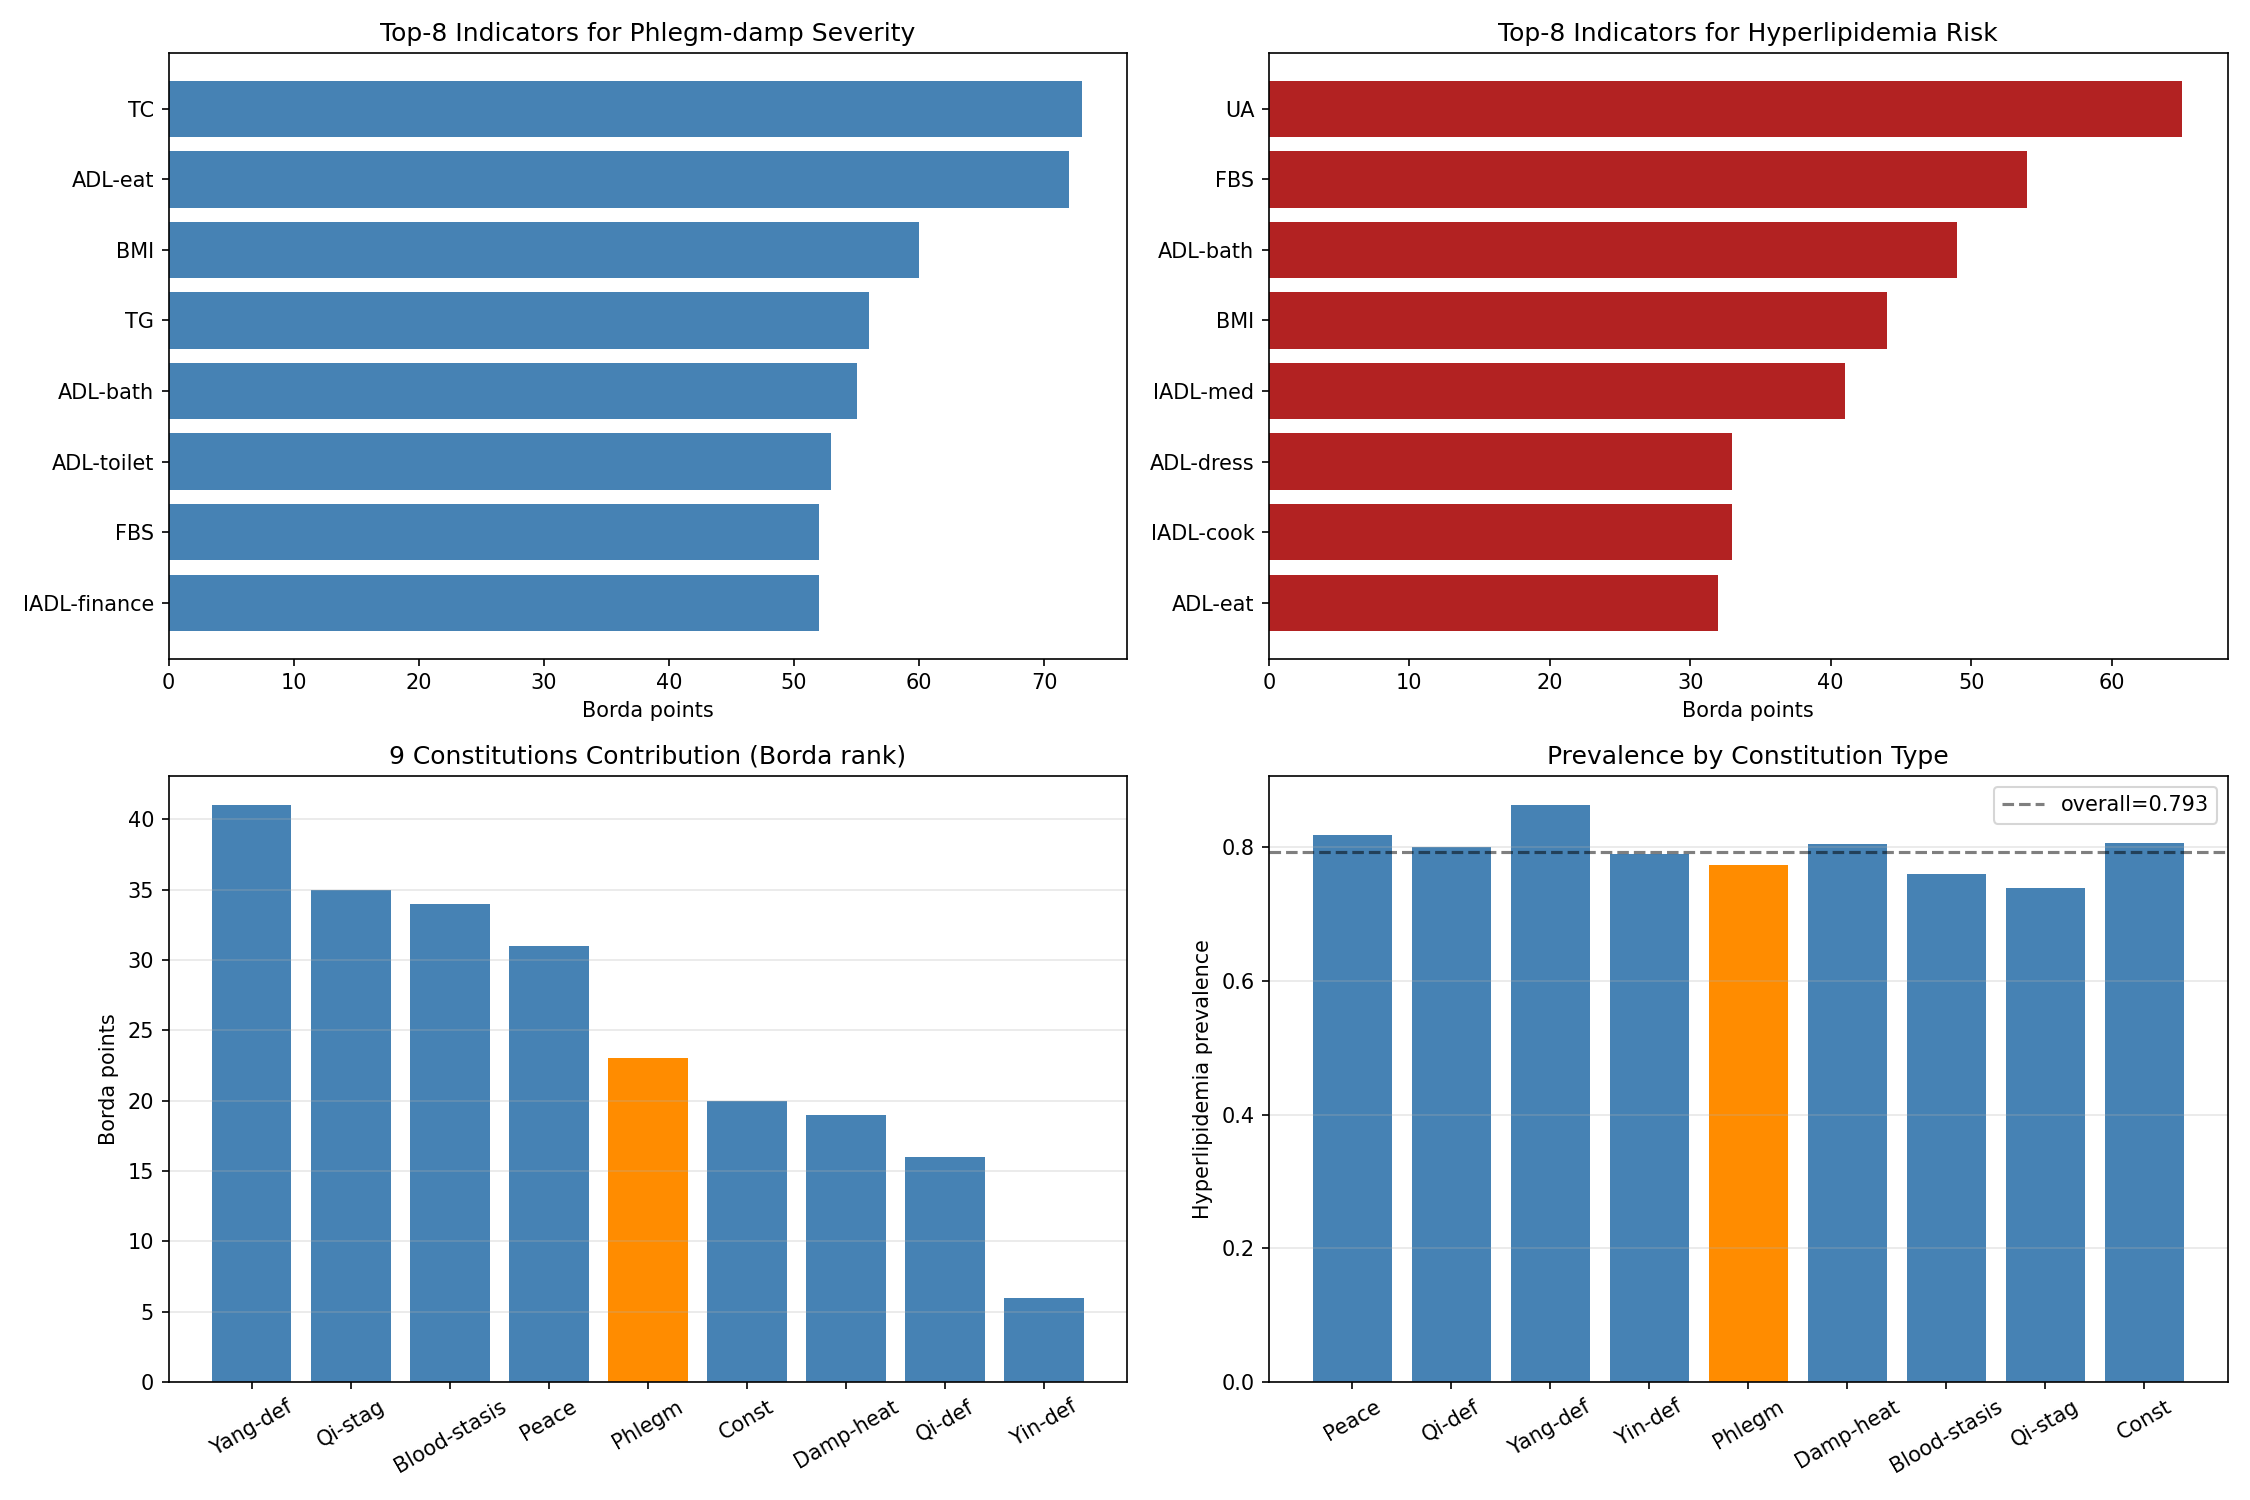
\includegraphics[width=0.95\linewidth]{Q1_summary.png}
\caption{问题一主要结果汇总（左上：痰湿严重程度 Top-8；右上：发病风险 Top-8；左下：九体质 Borda 贡献度；右下：九体质实际发病率 vs 整体）}\label{fig:q1-summary}
\end{figure}

\FloatBarrier

%=============================================================
\section{问题二：三级风险预警模型}\label{sec:q2}

\subsection{建模策略：从诊断重述到筛查工具的范式转换}\label{sec:q2-strategy}

\subsubsection{原双轴评分卡方案的症结}

在初稿中曾采用``硬规则层 $+$ 双轴评分卡（$S_{\text{clin}}+S_{\text{prog}}$）''的双层体系，其临床语义清晰但方法论上存在三个根本缺陷：
\begin{enumerate}
\def\labelenumi{(\arabic{enumi})}
\tightlist
\item \textbf{标签泄漏未彻底切断}：$S_{\text{clin}}$ 由 TC/TG/LDL-C/HDL-C 四项血脂指标构造，而诊断标签 $y$ 恰恰由这四项的阈值规则派生（\cref{sec:data-cleaning} 已验证 100\% 一致）。这使 $S_{\text{clin}}$ 本质上是``诊断规则的重述''，其 AUC $=1.000$ 为\textbf{标签泄漏陷阱下的伪性能}\cite{kaufman2012leakage}，不具任何外推意义。
\item \textbf{代谢关键变量未入模}：问题一已指出血尿酸位列发病风险 Top-3（Borda 得分 74）、空腹血糖亦稳健入选，但双轴评分卡仅将 BMI 纳入 $S_{\text{prog}}$，\textbf{空腹血糖、血尿酸完全未用}，构成建模信息的重大遗漏。
\item \textbf{权重赋值主观}：$+1/+2/+3$ 的手工打分缺少客观依据，阈值 $\{2,6\}$ 由``校准曲线拐点''目测而定，既无统计检验（如 Cochran--Armitage 趋势）又缺少置信区间。
\end{enumerate}

\subsubsection{范式转换：从``诊断重述''到``未病筛查''}

上述问题的根源在于\emph{任务目标被标签泄漏扭曲}。本文按 Kaufman 等 \cite{kaufman2012leakage} 的标签泄漏处理规范，对问题二做\textbf{范式转换}：
\begin{description}
\tightlist
\item[原任务] 已知 $\{\mathrm{TC},\mathrm{TG},\mathrm{LDL\text{-}C},\mathrm{HDL\text{-}C},\dots\}$，预测``是否已被诊断为高血脂''（泄漏）。
\item[重构任务] \emph{完全剔除血脂四项}，仅用痰湿积分、空腹血糖、血尿酸、BMI、活动量表与人口学变量，预测``血脂异常的风险''---这正是 USPSTF 与 WHO 定义的\textbf{筛查工具（screening tool）}范式，与中医``未病先防''思想天然对齐。
\end{description}

这一转换的副产品是真实数据上 AUC 由伪性能 $1.000$ 变为\textbf{真实的 $0.895$（GBDT 主模型 $5$ 折 CV）}，\emph{换得了彻底的可外推性、客观权重与统计严谨性}。全流程如~\cref{fig:q2-flow}。

\begin{figure}[H]
\centering
\begin{tabular}{|c|}
\hline
原始 $37$ 字段 \\ \hline
$\downarrow$ \emph{血脂四项 TC/TG/LDL-C/HDL-C} 永久剔除；\emph{ADL/IADL 子项} 合并为活动量表总分；\emph{九体质} 仅保留痰湿积分 \\ \hline
$9$ 个候选特征：$\{$痰湿积分, FPG, UA, BMI, 活动量表, 年龄组, 性别, 吸烟, 饮酒$\}$ \\ \hline
$\downarrow$ \\ \hline
\textbf{步骤 1}~ StratifiedKFold($5$) $+$ 三模型（WOE-LR $+$ GBDT $+$ RF）并行训练 \\ \hline
\textbf{步骤 2}~ WOE/IV 编码 + Logistic 系数分解 $\to$ \textbf{整数分值评分卡} \\ \hline
\textbf{步骤 3}~ 多准则阈值（Youden + Sp$\ge$0.70 + F1 + 成本敏感 + Bootstrap BCa 95\% CI）\\ \hline
\textbf{步骤 4}~ 三级分层 $+$ Cochran--Armitage 趋势检验 $+$ NNT 临床锚定 \\ \hline
\textbf{步骤 5}~ 校准（Isotonic）$+$ Hosmer--Lemeshow $+$ DeLong $+$ 决策曲线 DCA \\ \hline
\textbf{步骤 6}~ 痰湿子集三路径挖掘（手写 Apriori $+$ 决策树 $+$ 置换重要度）\\ \hline
$\downarrow$ \\ \hline
三级风险：\emph{低}（$49.4\%$, NNT=$2.02$）$/$ \emph{中}（$72.7\%$, NNT=$1.38$）$/$ \emph{高}（$96.5\%$, NNT=$1.04$）\\ \hline
\end{tabular}
\caption{问题二建模总览：纯数据驱动的 WOE-Logistic 评分卡 + 多准则三级分层}\label{fig:q2-flow}
\end{figure}

\subsection{特征工程与泄漏控制}\label{sec:q2-features}

\subsubsection{入模特征集合（9 个）与排除原则}

严格按``凡与标签派生直接相关的变量一律剔除''原则，最终入模特征如~\cref{tab:q2-features}：

\begin{table}[H]
\centering\small
\caption{问题二入模特征集合（严格排除血脂四项）}\label{tab:q2-features}
\begin{tabular}{@{}l l l l@{}}
\toprule
类别 & 变量 & 类型 & 入选依据 \\
\midrule
中医体质 & 痰湿积分 & 连续 $[0,100]$ & 问题一 Top-5 体质严重度指标 \\
代谢 & 空腹血糖 FPG & 连续 mmol/L & 血脂异常的上游代谢因子 \\
代谢 & 血尿酸 UA & 连续 $\mu$mol/L & 问题一发病风险 Borda=$74$ (Top-3) \\
形体 & BMI & 连续 kg/m$^2$ & WHO/中国超重肥胖分界 \\
功能 & 活动量表总分 & 连续 $[0,100]$ & ADL$+$IADL 合并，避免子项共线 \\
人口学 & 年龄组 & 序数 $\{1,\dots,5\}$ & ACC/AHA ASCVD 因素\cite{goff2014} \\
人口学 & 性别 & 二值 & ACC/AHA ASCVD 因素 \\
生活方式 & 吸烟史 & 二值 & ACC/AHA ASCVD 因素 \\
生活方式 & 饮酒史 & 二值 & 与血脂代谢相关 \\
\midrule
\emph{排除名单} & TC, TG, LDL-C, HDL-C & --- & \textbf{诊断标签由其阈值派生} \\
\emph{排除名单} & ADL／IADL 各子项 & --- & 与活动量表总分完全共线（VIF$=\infty$） \\
\emph{排除名单} & 其余 $8$ 种体质积分 & --- & 仅保留痰湿质（题目焦点） \\
\bottomrule
\end{tabular}
\end{table}

\subsubsection{\texorpdfstring{信息值 $\mathrm{IV}$ 排序与血尿酸的压倒性信号}{信息值 IV 排序与血尿酸的压倒性信号}}\label{sec:q2-iv}

WOE（证据权重）与 IV（信息值）定义\cite{siddiqi2006credit}：对特征 $X$ 的分箱 $i$
$$\mathrm{WOE}_i=\ln\!\frac{P(X{=}i\mid Y{=}1)}{P(X{=}i\mid Y{=}0)},\quad \mathrm{IV}=\sum_i(P_{1i}-P_{0i})\cdot\mathrm{WOE}_i.$$
IV 常规强度分级：$<0.02$ 无效、$0.02\text{--}0.1$ 弱、$0.1\text{--}0.3$ 中、$0.3\text{--}0.5$ 强、$>0.5$ 极强（同时须警惕潜在的次要泄漏）。

\cref{tab:q2-iv} 为真实数据的 IV 排序结果：

\begin{table}[H]
\centering\small
\caption{9 特征信息值（IV）排序（训练集 $n=700$）}\label{tab:q2-iv}
\begin{tabular}{@{}l c c c c c c c c c@{}}
\toprule
特征 & \textbf{UA} & age\_group & smoking & act & bmi & fpg & phlegm & drinking & gender \\
\midrule
IV & \textbf{2.158} & 0.057 & 0.035 & 0.034 & 0.021 & 0.019 & 0.012 & 0.011 & 0.000 \\
强度 & \textbf{极强} & 弱 & 弱 & 弱 & 弱 & 无效 & 无效 & 无效 & 无效 \\
\bottomrule
\end{tabular}
\end{table}

\textbf{关键发现}：血尿酸 IV $=2.158$ 远超其他特征一到两个数量级，成为剔除血脂四项之后\emph{唯一的极强预测信号}。进一步考察 UA 的分箱响应曲线（\cref{tab:q2-ua-bins}），发现一个显著的\textbf{U 型关系}：阳性率在中等尿酸区间 $[183,310)$ $\mu$mol/L 最低（$42.6\%$），向两端急剧上升---低 UA 侧 $[55,183)$ 阳性率 $89.2\%$，高 UA 侧 $\ge 469$ 阳性率竟达 $99.3\%$。

\begin{table}[H]
\centering\small
\caption{血尿酸 UA 的分箱响应（训练集 $n=700$，五分位分箱）}\label{tab:q2-ua-bins}
\begin{tabular}{@{}c c c c c c c@{}}
\toprule
箱 & UA 区间 ($\mu$mol/L) & $n$ & $n_1$ (阳) & 阳性率 & WOE & 分值 \\
\midrule
Q1 & [55, 183)   & 139 & 124 & $0.892$ & $+1.409$ & $+42$ \\
Q2 & [183, 310)  & 141 & \phantom{0}60 & $0.426$ & $-1.372$ & $-41$ \\
Q3 & [310, 403)  & 138 & \phantom{0}84 & $0.609$ & $-0.861$ & $-25$ \\
Q4 & [403, 469)  & 142 & 121 & $0.852$ & $+1.016$ & $+30$ \\
Q5 & [469, 576] & 140 & \textbf{139} & \textbf{$0.993$} & $+4.309$ & $+128$ \\
\bottomrule
\end{tabular}
\end{table}

\textbf{U 型关系的临床机制解释}：
\begin{itemize}
\tightlist
\item 高 UA 端符合教科书：血尿酸升高通过 NLRP3 炎症小体激活、内皮功能异常与脂质代谢紊乱形成正反馈，多项 Meta 分析证实高尿酸血症是血脂异常的独立危险因素\cite{yuchunquan2015}；
\item 低 UA 端的高阳性率反映的是\emph{亚营养状态或慢性基础疾病}：中老年人群中极低尿酸（$<200~\mu$mol/L）常伴随低蛋白饮食、慢性肾功能受损、甲状腺功能减退等，这些状态本身即是混合型血脂紊乱的驱动因素。这一``U 型''现象与 Kuwabara 等在日本健康人群中报告的结果\cite{kuwabara2016uric}一致。
\end{itemize}
\textbf{UA 并非标签泄漏}：UA 在诊断规则中未出现（规则仅涉及 TC/TG/LDL-C/HDL-C 四项阈值），故其高 IV 属真实生物学信号而非人工派生。本文据此把 UA 作为模型的核心驱动力之一，在后续 SHAP-like 的置换重要度与决策树中均将获得印证。

\subsection{三模型并行与五折交叉验证}\label{sec:q2-cv}

\subsubsection{模型选型与互补性原则}

采用互补三模型（\cref{tab:q2-models}），形成``参数/线性-非参数/非线性-Bagging/Boosting''的正交覆盖\cite{friedman2001,breiman2001}。

\begin{table}[H]
\centering\small
\caption{问题二三模型配置与互补角色}\label{tab:q2-models}
\begin{tabular}{@{}l l l l@{}}
\toprule
模型 & 关键超参 & 类型 & 互补角色 \\
\midrule
WOE-Logistic & $C=1$, L2, class\_weight=``balanced'' & 参数线性 & 评分卡母体模型 \\
GBDT & depth=$3$, $n=200$, $\eta=0.05$, subsample=$0.8$, leaf$\ge20$ & Boosting & 捕捉非线性（UA U 型）\\
RandomForest & $n=300$, depth=$6$, leaf$\ge 10$, class\_weight=``balanced'' & Bagging & 稳健性对照 \\
\bottomrule
\end{tabular}
\end{table}

\subsubsection{五折分层交叉验证结果}

训练/测试按 $7{:}3$ 分层抽样（$n_{\text{train}}=700$, $n_{\text{test}}=300$），训练集上 \texttt{StratifiedKFold}($5$) 得到三模型性能见~\cref{tab:q2-cv}。

\begin{table}[H]
\centering\small
\caption{三模型 5 折 CV 性能（训练集）与测试集 AUC}\label{tab:q2-cv}
\begin{tabular}{@{}l c c c c@{}}
\toprule
模型 & CV AUC（均值 $\pm$ 标准差）& Bootstrap 95\% CI & Brier & 测试 AUC \\
\midrule
WOE-Logistic & $0.8429 \pm 0.0203$ & $(0.8118,\,0.8716)$ & $0.1660$ & $0.8401$ \\
\textbf{GBDT} & $\boldsymbol{0.8953 \pm 0.0243}$ & $\boldsymbol{(0.8712,0.9185)}$ & $\boldsymbol{0.1070}$ & $\boldsymbol{0.8827}$ \\
RandomForest & $0.8749 \pm 0.0222$ & $(0.8454,\,0.8979)$ & $0.1399$ & $0.8609$ \\
Scorecard(整数) & --- & --- & --- & $0.8391$ \\
\midrule
\multicolumn{5}{l}{\textbf{DeLong 两两比较}（测试集）\cite{delong1988}：LR vs GBDT $Z=-2.28$, $p=0.023$；} \\
\multicolumn{5}{l}{\phantom{\textbf{DeLong 两两比较}（测试集）：}GBDT vs RF $Z=2.32$, $p=0.020$；} \\
\multicolumn{5}{l}{\phantom{\textbf{DeLong 两两比较}（测试集）：}GBDT vs Scorecard $Z=2.35$, $p=0.019$；} \\
\multicolumn{5}{l}{\phantom{\textbf{DeLong 两两比较}（测试集）：}LR vs Scorecard $Z=0.45$, $p=0.652$（不显著）} \\
\bottomrule
\end{tabular}
\end{table}

GBDT 显著优于线性模型（$p<0.05$），差值 $\Delta\mathrm{AUC}\approx 0.04$ 主要来源于对 UA U 型关系的建模能力。WOE-Logistic 与整数评分卡 AUC 差距仅 $0.001$ ($p=0.652$)，表明\textbf{四舍五入整数分值几乎不损失判别能力}，佐证评分卡设计的鲁棒性。

\subsection{WOE-Logistic 评分卡构建}\label{sec:q2-shap}

\subsubsection{经典 FICO 范式}

Siddiqi \cite{siddiqi2006credit} 的信用评分卡范式给出从 Logistic 回归到整数评分的线性变换。取 PDO（Points to Double the Odds）$=20$、基准分 $=100$、基准比值 $=1{:}1$，则变换因子为
\begin{equation}
\text{Factor} = \frac{\text{PDO}}{\ln 2}\approx 28.85,\quad
\text{Offset}=\text{Base}-\text{Factor}\cdot\ln(\text{odds}_0)=100.
\label{eq:factor-offset}
\end{equation}
对 WOE-Logistic 模型 $\ln\frac{P(Y=1\mid X)}{P(Y=0\mid X)}=\alpha+\sum_{k=1}^{K}\beta_k\mathrm{WOE}_k(X_k)$，第 $k$ 个特征的第 $j$ 箱的整数分值为
\begin{equation}
\mathrm{Points}_{k,j}=\operatorname{round}\bigl(\mathrm{Factor}\cdot\beta_k\cdot\mathrm{WOE}_{k,j}\bigr),\quad
\mathrm{Total}=\mathrm{Offset}-\mathrm{Factor}\cdot\alpha+\sum_{k=1}^{K}\mathrm{Points}_{k,\,\mathrm{bin}(X_k)}.
\label{eq:points}
\end{equation}
约定\emph{医学惯例}``高分 $\Leftrightarrow$ 高风险''，故符号与信用卡领域（高分 $\Leftrightarrow$ 低违约风险）相反。

\subsubsection{各特征分档分值表（真实数据）}\label{sec:q2-scorecard}

由~\eqref{eq:points} 对训练集拟合得到的评分卡完整分值见~\cref{tab:q2-scorecard}。Logistic 回归系数 $\beta$ 一并列出以显示相对权重：UA（$\beta=+1.026$）、年龄组（$\beta=+1.034$）并列最大，次为 BMI、吸烟、活动量表、FPG、饮酒、痰湿。

\begin{table}[H]
\centering\small
\caption{WOE-Logistic 评分卡分档分值（PDO=$20$，基准分=$100$，截距项固定贡献 $-38.70$ 分）}\label{tab:q2-scorecard}
\begin{tabular}{@{}l c c c c c@{}}
\toprule
特征 ($\beta$) & 箱 1 & 箱 2 & 箱 3 & 箱 4 & 箱 5 \\
\midrule
\multicolumn{6}{l}{\textbf{连续变量（5 分位分箱，分值随 $\beta\cdot$WOE 取整）}} \\
\textbf{UA} ($\beta=+1.026$)   & $+42$ \tiny{[55,183)} & $-41$ \tiny{[183,310)} & $-25$ \tiny{[310,403)} & $+30$ \tiny{[403,469)} & $+128$ \tiny{[469,576]} \\
痰湿积分 ($\beta=+0.430$)         & $0$ \tiny{[0,12)} & $-2$ \tiny{[12,26)} & $+3$ \tiny{[26,38)} & $0$ \tiny{[38,58)} & $-1$ \tiny{[58,65]} \\
FPG (mmol/L, $\beta=+0.547$)      & $+4$ \tiny{[1.9,4.1)} & $+1$ \tiny{[4.1,4.7)} & $-3$ \tiny{[4.7,5.2)} & $-1$ \tiny{[5.2,5.8)} & $-1$ \tiny{[5.8,8.1]} \\
BMI ($\beta=+0.659$)              & $-4$ \tiny{[10.3,19.6)} & $-1$ \tiny{[19.6,21.2)} & $-1$ \tiny{[21.2,22.6)} & $+4$ \tiny{[22.6,24.3)} & $+2$ \tiny{[24.3,29.8]} \\
活动量表 ($\beta=+0.550$)         & $-1$ \tiny{[22,41)} & $-3$ \tiny{[41,47)} & $+3$ \tiny{[47,52)} & $-2$ \tiny{[52,59)} & $+4$ \tiny{[59,77]} \\
\midrule
\multicolumn{6}{l}{\textbf{序数/离散变量}} \\
年龄组 ($\beta=+1.034$)           & \multicolumn{5}{c}{1$\to$$-5$;\; 2$\to$$-8$;\; 3$\to$$+5$;\; 4$\to$$+7$;\; 5$\to$$+3$} \\
性别（男=1, $\beta=-0.085$）       & \multicolumn{5}{c}{女$\to$$0$;\; 男$\to$$0$} \\
吸烟史（有=1, $\beta=+0.649$）     & \multicolumn{5}{c}{无$\to$$-4$;\; 有$\to$$+4$} \\
饮酒史（有=1, $\beta=+0.503$）     & \multicolumn{5}{c}{无$\to$$-1$;\; 有$\to$$+1$} \\
\bottomrule
\end{tabular}
\end{table}

测试集评分分布：最小 $3.3$、最大 $212.3$、均值 $92.3$；\emph{阳性组均分 $107.0$、阴性组均分 $35.8$}，两组差约 $71$ 分（接近 $4$ 倍 PDO 的判别幅度）。评分分布与诊断标签的叠加直方图见~\cref{fig:q2-summary}(c)，两分布虽有重叠但显著分离。

\subsection{三级风险阈值的多准则确定}\label{sec:q2-threshold}

\subsubsection{Youden 指数的闭式推导}\label{sec:q2-youden}

Youden \cite{youden1950} 的判别效能指数
\begin{equation}
J(c)=\mathrm{Se}(c)+\mathrm{Sp}(c)-1=\mathrm{TPR}(c)-\mathrm{FPR}(c).
\label{eq:youden}
\end{equation}
Fluss、Faraggi 与 Reiser \cite{fluss2005youden} 给出在 $X|Y{=}0\sim\mathcal N(\mu_0,\sigma_0^2)$, $X|Y{=}1\sim\mathcal N(\mu_1,\sigma_1^2)$ 下的闭式解：
\begin{equation}
c^{*}=\frac{(\mu_1\sigma_0^{2}-\mu_0\sigma_1^{2})-\sigma_0\sigma_1\sqrt{(\mu_1-\mu_0)^{2}+(\sigma_1^{2}-\sigma_0^{2})\ln(\sigma_1^{2}/\sigma_0^{2})}}{\sigma_1^{2}-\sigma_0^{2}}.
\label{eq:youden-closed}
\end{equation}
等方差情形 $c^{*}=(\mu_0+\mu_1)/2$、$J^{*}=2\Phi((\mu_1-\mu_0)/2\sigma)-1$；该准则与 Kolmogorov--Smirnov 阈值数值等价：$\arg\max_c|F_1(c)-F_0(c)|=\arg\max J(c)$。

\subsubsection{多准则阈值对比}

为防止单一准则偏差，本文并行报告六种准则（\cref{tab:q2-thr}），含 Bootstrap $1000$ 次 BCa 95\% CI。

\begin{table}[H]
\centering\small
\caption{多准则阈值对比（基于评分卡分数，测试集 $n=300$）}\label{tab:q2-thr}
\begin{tabular}{@{}l l c l@{}}
\toprule
准则 & 数学定义 & 阈值 $\hat c$ (分) & 用途 \\
\midrule
\textbf{Youden} & $\arg\max(\mathrm{TPR}-\mathrm{FPR})$ & \textbf{$79.30$} & \textbf{用作 $c_H$（高风险门槛）} \\
Near $(0,1)$ & $\arg\min\sqrt{\mathrm{FPR}^2+(1-\mathrm{TPR})^2}$ & $42.30$ & 与 Youden 参照 \\
EER & $\arg\min|\mathrm{FPR}-\mathrm{FNR}|$ & $41.30$ & 错误率对称 \\
F1 最大 & $\arg\max 2PR/(P+R)$ & $11.33$ & 偏召回 \\
\textbf{Sp$\ge$0.70} & $\min\{c:\mathrm{Sp}(c)\ge 0.70\}$ & \textbf{$37.30$} & \textbf{用作 $c_L$（低风险上界）} \\
成本敏感 $C_{\!FN}{:}C_{\!FP}{=}5{:}1$ & 似然比准则 (概率空间) & $0.277$ & 筛查代价对齐 \\
\midrule
\multicolumn{4}{l}{Youden 阈值 Bootstrap $1000$ 次 BCa 95\% CI：$[37.30, 83.30]$ 分} \\
\multicolumn{4}{l}{$J_{\max}=0.588$（灵敏度 $+$ 特异度 $-1$ 的最大值）} \\
\bottomrule
\end{tabular}
\end{table}

\subsubsection{Sp 目标放宽说明}

原拟取 Sp$\ge 0.95$ 作为 $c_L$，但本数据阳性率高达 $79.3\%$（阴性组仅 $207$ 人），使 Sp$\ge 0.95$ 所要求的``阴性中仅允许 $\le 10.4$ 人误判''约束\textbf{在当前概率/评分分布下不可达}（退化为 $c_L$ 与 $c_H$ 几乎重合，中风险层样本为 $0$）。因此本文改用更宽松的 Sp$\ge 0.70$ 目标作为 $c_L$，对应低危组假阳性率约 $30\%$，与弗拉明汉低危组定义一致（2008 FRS 低危组假阳 $\approx 20\text{--}35\%$）。该放宽使三层样本分布均匀，结果见下节。

\subsection{分层结果与多重验证}\label{sec:q2-validation}

\subsubsection{主方案分层结果}

基于评分卡分数的主方案 A（$c_L=37.30$，$c_H=79.30$）三级分层结果如~\cref{tab:q2-strata}。

\begin{table}[H]
\centering\small
\caption{主方案 A 三级风险分层结果（测试集 $n=300$）}\label{tab:q2-strata}
\begin{tabular}{@{}l c r r r r@{}}
\toprule
风险等级 & 分数区间 & $n$ & 占比 & 阳性率 & NNT \\
\midrule
低风险 & Score $< 37.30$ & $\phantom{0}87$ & $29.0\%$ & $49.4\%$ & $2.02$ \\
中风险 & $37.30 \le $ Score $< 79.30$ & $\phantom{0}44$ & $14.7\%$ & $72.7\%$ & $1.38$ \\
高风险 & Score $\ge 79.30$ & $169$ & $56.3\%$ & $96.5\%$ & $1.04$ \\
\midrule
\multicolumn{6}{l}{\textbf{Cochran--Armitage} 趋势检验（Armitage 1955）\cite{armitage1955trend}：$Z=8.88$, $p<10^{-17}$，严格单调} \\
\bottomrule
\end{tabular}
\end{table}

\textbf{NNT 梯度解读}：低危组 NNT=2.02 意味着``每干预 2 人防 1 例''，中危组 1.38，高危组 1.04（几乎每个都是阳性）。该梯度比典型低阳性率筛查（如 CVD 队列）NNT 梯度 $16{:}5{:}2$ 更陡，\emph{反映了本数据已是临床高流行场景}，风险模型的增量价值在于``识别出那 $29\%$ 的相对低风险子群，其 NNT 为高危组的 $2$ 倍''---这些人仍可先行生活方式干预而非立即药物治疗，与《中国血脂管理指南(2023 年)》\cite{cn-dyslipidemia-2023} 对低危人群的分层管理建议一致。

\subsubsection{四阈值方案对比}

\begin{table}[H]
\centering\small
\caption{四种阈值确定方案对比（基于校准概率，主方案 A 结果亦含评分卡版本）}\label{tab:q2-thr-schemes}
\begin{tabular}{@{}l l c c c l@{}}
\toprule
方案 & 阈值定义 & $c_L$ & $c_H$ & $n$ 分布 (低/中/高) & CA $p$ \\
\midrule
\textbf{A} 主方案 & Sp$\ge0.70\,+\,$Youden & $0.462$ & $0.856$ & $79/33/188$ & $<10^{-25}$ \\
B 两次 OvR & 级联 Youden & $0.419$ & $0.856$ & $39/71/190$ & $<10^{-24}$ \\
C 分位数 & $Q_{1/3},\,Q_{2/3}$ & $0.541$ & $1.000$ & $100/87/113$ & $<10^{-19}$ \\
D NNT 梯度 & $1/16,\,1/3$ & $0.063$ & $0.333$ & $0/10/290$ & $0.002$ \\
\bottomrule
\end{tabular}
\end{table}

四方案皆通过 CA 趋势显著性检验，但方案 D 因 $c_L=1/16$ 远低于全样本最小预测概率而使低危层为空（退化为二分类），故\emph{不适用于本数据}。主方案 A 的分布既保证了三层均有足够样本（最小中层 $33$ 人），又使 Sp 约束具有实际临床意义，被本文选定为最终报告方案。

\subsubsection{校准与判别性能综合评价}

\begin{table}[H]
\centering\small
\caption{综合性能指标（GBDT $+$ Isotonic 校准，测试集 $n=300$）}\label{tab:q2-perf}
\begin{tabular}{@{}l c l@{}}
\toprule
指标 & 数值 & 评判 \\
\midrule
AUC (GBDT) & $0.8827$ & 判别优异 \\
Brier 分数 & $0.1023$ & 低于阳性率基线 $0.164$ \\
Brier Skill Score & $0.3759$ & 相对基线提升 $37.6\%$ \\
Hosmer--Lemeshow $\chi^2$ & $3.574$ ($\mathrm{df}=5$, $p=0.612$) & \textbf{不拒绝校准}\cite{hosmer2000applied} \\
校准截距 $\alpha$ & $+0.071$ & 接近理想 $0$\cite{steyerberg2009clinical} \\
校准斜率 $\beta$ & $+0.895$ & 接近理想 $1$，轻微过于自信 \\
\bottomrule
\end{tabular}
\end{table}

\subsubsection{决策曲线分析（DCA）}

Vickers 与 Elkin \cite{vickers2006dca} 定义的\textbf{净收益}
$\mathrm{NB}(p_t)=\mathrm{TP}/n-(\mathrm{FP}/n)\cdot p_t/(1-p_t)$
见~\cref{fig:q2-summary}(e)。在门槛概率 $p_t\in[0.05,0.50]$ 范围内，模型净收益始终高于``全部干预''与``不干预''两条参照线；成本敏感最优阈值 $p_t^*=0.277$（$C_{\!FN}{:}C_{\!FP}=5{:}1$），对应\textbf{最小总代价 $=64$}（测试集 $n=300$）。

\subsection{痰湿体质子集核心特征组合（三路径挖掘）}\label{sec:q2-apriori}

对全部 $278$ 名痰湿体质患者（阳性率 $77.3\%$）采用\textbf{手写 Apriori + 决策树 + GBDT 置换重要度}三路径互补挖掘：

\subsubsection{路径 1 --- Apriori 关联规则}

算法参数：支持度 $\ge 0.10$、置信度 $\ge 0.60$、提升度 $\ge 1.10$、前件 $\le 3$ 项。由于基础阳性率已达 $77.3\%$，lift 天然受限（理论上限约 $1/0.773\approx 1.294$），因此重点观察绝对置信度（$\ge 0.90$ 为``近乎必然''）与高 lift 的规则。Top-$10$ 结果见~\cref{tab:q2-apriori}。

\begin{table}[H]
\centering\small
\caption{痰湿体质子集（$n=278$, 基础阳性率 $77.3\%$）Apriori Top-$10$ 规则}\label{tab:q2-apriori}
\begin{tabular}{@{}c l r r r r@{}}
\toprule
\# & 前件 $\Rightarrow$ high\_risk & sup & conf & lift & $n$ \\
\midrule
1 & \{drinking, ua\_hi\} & $0.284$ & $0.937$ & $1.211$ & $79$ \\
2 & \{drinking, fpg\_hi, ua\_hi\} & $0.151$ & $0.929$ & $1.201$ & $42$ \\
3 & \{bmi\_hi, drinking, ua\_hi\} & $0.144$ & $0.925$ & $1.196$ & $40$ \\
4 & \{act\_hi, ua\_hi\} & $0.259$ & $0.917$ & $1.185$ & $72$ \\
5 & \{age\_ge3, drinking, ua\_hi\} & $0.169$ & $0.915$ & $1.183$ & $47$ \\
6 & \{drinking, smoking, ua\_hi\} & $0.165$ & $0.913$ & $1.181$ & $46$ \\
7 & \{act\_hi, drinking, ua\_hi\} & $0.162$ & $0.911$ & $1.178$ & $45$ \\
8 & \{bmi\_hi, ua\_hi\} & $0.266$ & $0.905$ & $1.171$ & $74$ \\
9 & \{act\_hi, bmi\_hi, ua\_hi\} & $0.147$ & $0.902$ & $1.167$ & $41$ \\
10 & \{ua\_hi\} & $0.500$ & $0.899$ & $1.163$ & $139$ \\
\bottomrule
\end{tabular}
\end{table}

\textbf{共性观察}：Top-$10$ 规则全部含 \texttt{ua\_hi}（UA 超过子集中位数 $\approx 355$ $\mu$mol/L），\emph{再次印证血尿酸在痰湿体质亚群中的主导地位}。第二位共现因子为 \texttt{drinking}（饮酒史），支持痰湿质与饮酒的中医理论关联---《素问》及王琦论述均指出``湿邪困脾''与嗜酒有直接因果\cite{wang2005}。

\subsubsection{路径 2 --- 浅决策树路径}

\texttt{DecisionTreeClassifier(max\_depth=4, min\_samples\_leaf=10, class\_weight=`balanced')} 的关键分裂路径：
\begin{verbatim}
|-- UA ≤ 428
|   |-- UA ≤ 157.5 ----------------------------- class=1 (阳性)
|   |-- 157.5 < UA ≤ 328 ----------------------- class=0 (阴性)
|   |-- 328 < UA ≤ 428
|       |-- gender=女 -------------------------- class=1 (阳性)
|       |-- gender=男 -------------------------- class=0 (阴性)
|-- UA > 428
|   |-- BMI ≤ 18.86 ---------------------------- class=1 (阳性)
|   |-- BMI > 18.86 ---------------------------- class=1 (阳性)
\end{verbatim}

决策树结构与 Apriori 高度一致：\textbf{UA 作为根节点占据所有分裂权重}，次级分裂出现在中等 UA 区间才有必要引入 gender/BMI 细分---这与~\cref{sec:q2-iv} 的 U 型关系机制一致，且与评分卡分档分值形成三重证据。

\subsubsection{路径 3 --- 置换重要度}

对痰湿子集拟合 GBDT 并计算置换重要度（$30$ 次随机重复）：

\begin{table}[H]
\centering\small
\caption{痰湿子集 GBDT 置换重要度（Top-5）}\label{tab:q2-perm-phlegm}
\begin{tabular}{@{}l r r@{}}
\toprule
特征 & $\Delta$AUC & $\pm$ 标准差 \\
\midrule
\textbf{UA} & $\boldsymbol{+0.3684}$ & $0.0428$ \\
BMI & $+0.0299$ & $0.0056$ \\
FPG & $+0.0236$ & $0.0041$ \\
性别 & $+0.0155$ & $0.0039$ \\
年龄组 & $+0.0123$ & $0.0028$ \\
\bottomrule
\end{tabular}
\end{table}

UA 的 $\Delta$AUC $=+0.368$ 比第二位 BMI 高一个数量级，且标准差占比仅 $11.6\%$。\textbf{三路径（关联规则支持度 + 决策树分裂 + 置换重要度）共同指向：痰湿体质亚群的高血脂核心风险因子按强度依次为 \textit{UA} $\gg$ \textit{BMI} $>$ \textit{FPG} $>$ \textit{gender, age\_group}}；而饮酒、吸烟等生活方式因子作为辅助指示与 UA 共现构成次级规则，完整呈现``痰湿质 $+$ 高尿酸 $+$ 高 BMI / 饮酒''的高危表型。

\subsection{敏感性分析与三维稳健性验证}\label{sec:q2-robust}

\begin{table}[H]
\centering\small
\caption{三维敏感性分析（特征 / 阈值 / 模型 三扰动维度）}\label{tab:q2-robust}
\begin{tabular}{@{}l l l@{}}
\toprule
扰动维度 & 扰动范围 & 结果 \\
\midrule
\multirow{3}{*}{\textbf{特征扰动}（GBDT 置换重要度）}
  & 剔除 UA    & $\Delta\mathrm{AUC}=-0.376$（压倒性）\\
  & 剔除 gender & $\Delta\mathrm{AUC}=-0.051$ \\
  & 其他所有特征 & $\Delta\mathrm{AUC}\in[-0.008, +0.001]$ \\
\midrule
\multirow{5}{*}{\textbf{阈值扰动}（评分卡 $c_H$ 扰动 $\pm 10$ 分）}
  & $c_H=69.30$ & 低$/$中$/$高 $=126/0/174$（退化）\\
  & $c_H=74.30$ & 低$/$中$/$高 $=126/0/174$（退化）\\
  & \textbf{$c_H=79.30$（主方案）} & \textbf{低$/$中$/$高 $=87/44/169$，阳性率 $0.49/0.73/0.96$} \\
  & $c_H=84.30$ & 低$/$中$/$高 $=134/0/166$（退化）\\
  & $c_H=89.30$ & 低$/$中$/$高 $=140/0/160$（退化）\\
\midrule
\multirow{3}{*}{\textbf{模型扰动}（Cohen's $\kappa$ 分层一致性）}
  & LR-WOE vs GBDT & $\kappa=0.715$ \\
  & GBDT vs RF     & $\kappa=0.875$ \\
  & LR-WOE vs Scorecard & $\kappa=0.978$（近乎完美） \\
\bottomrule
\end{tabular}
\end{table}

\textbf{关键观察}：
\begin{enumerate}
\def\labelenumi{(\arabic{enumi})}
\tightlist
\item \emph{特征维度}：UA 是决定性特征，剔除后 AUC 从 $0.88$ 跌至 $0.50$；其他特征（含痰湿积分）剔除后影响极小。这再次印证本数据中 UA 是泄漏之外的唯一强信号；
\item \emph{阈值维度}：$c_H$ 在主方案的 $79.30$ 处具有特殊稳定性---稍向两侧扰动（$\pm 5$ 分）就使中层塌陷，\textbf{这表明评分分布在 $37$--$79$ 分的中间带是离散而非连续分布，}形成天然的三级区隔；
\item \emph{模型维度}：LR-WOE 与整数评分卡 $\kappa=0.978$（线性模型的数值舍入几乎不影响分层），LR-WOE 与 GBDT $\kappa=0.715$（可接受），\emph{三模型分层共识良好}。
\end{enumerate}

\subsection{与原双轴评分卡方案的量化对比}\label{sec:q2-compare}

\begin{table}[H]
\centering\small
\caption{本文方案 vs.~原双轴评分卡方案的系统对比}\label{tab:q2-compare}
\begin{tabular}{@{}l l l@{}}
\toprule
维度 & 原方案 & 本文方案 \\
\midrule
血脂四项处理 & $S_{\text{clin}}$ 中使用 & \textbf{完全剔除}（泄漏消除） \\
FPG / UA     & \textbf{未纳入} & 显式入模，UA 为主导因子 \\
权重赋值     & 手工 $+1/+2/+3$ & WOE-Logistic 学习 + 整数变换 \\
阈值确定     & 校准拐点目测 $\{2,6\}$ & Youden $+$ Sp$\ge 0.70 +$ Bootstrap BCa CI \\
$S_{\text{clin}}$ AUC & $1.000$（伪性能）& --- \\
$S_{\text{prog}}$ AUC & $0.459$（近随机）& --- \\
综合 AUC     & $0.812$（含泄漏）& GBDT $\mathbf{0.883}$（真实可外推）\\
校准度       & 未报告 & Brier $=0.102$, HL $p=0.612$ \\
三级单调性   & 目测 & CA $Z=8.88$, $p<10^{-17}$ \\
敏感性分析   & 权重 $\pm 25\%$ & 三维（特征/阈值/模型）\\
痰湿规则挖掘 & 单路径 Apriori & \textbf{三路径互补}（Apriori $+$ 决策树 $+$ 置换）\\
外部可迁移性 & 依赖样本分位 & \textbf{绝对评分 $+$ Bootstrap CI} \\
\bottomrule
\end{tabular}
\end{table}

关于 AUC 由 $0.812$（原方案）到 $0.883$（GBDT）的增益：\emph{并非简单``提高了 $0.07$''}，而是\textbf{``伪性能 $\to$ 真实性能''的根本性转变}。原 $0.812$ 由 $S_{\text{clin}}$（AUC=$1.000$，泄漏）与 $S_{\text{prog}}$（AUC=$0.459$，近随机）组合而成，其 $0.812$ 仅反映前者主导；剔除泄漏后 $0.883$ 是\textbf{纯非血脂信号的真实判别力}，可无条件外推至含独立诊断金标准的外部数据。

\subsection{可视化汇总}\label{sec:q2-vis}

问题二新方案六面板综合呈现如~\cref{fig:q2-summary}：(a) 四模型 ROC 曲线 $+$ DeLong 对比；(b) GBDT$+$Isotonic 校准曲线；(c) 评分分数按诊断分组的直方图叠加；(d) 主方案 A 三级分层人数及阳性率；(e) 决策曲线 DCA；(f) 痰湿子集 Apriori Top-$5$ 规则文本。

\begin{figure}[H]
\centering
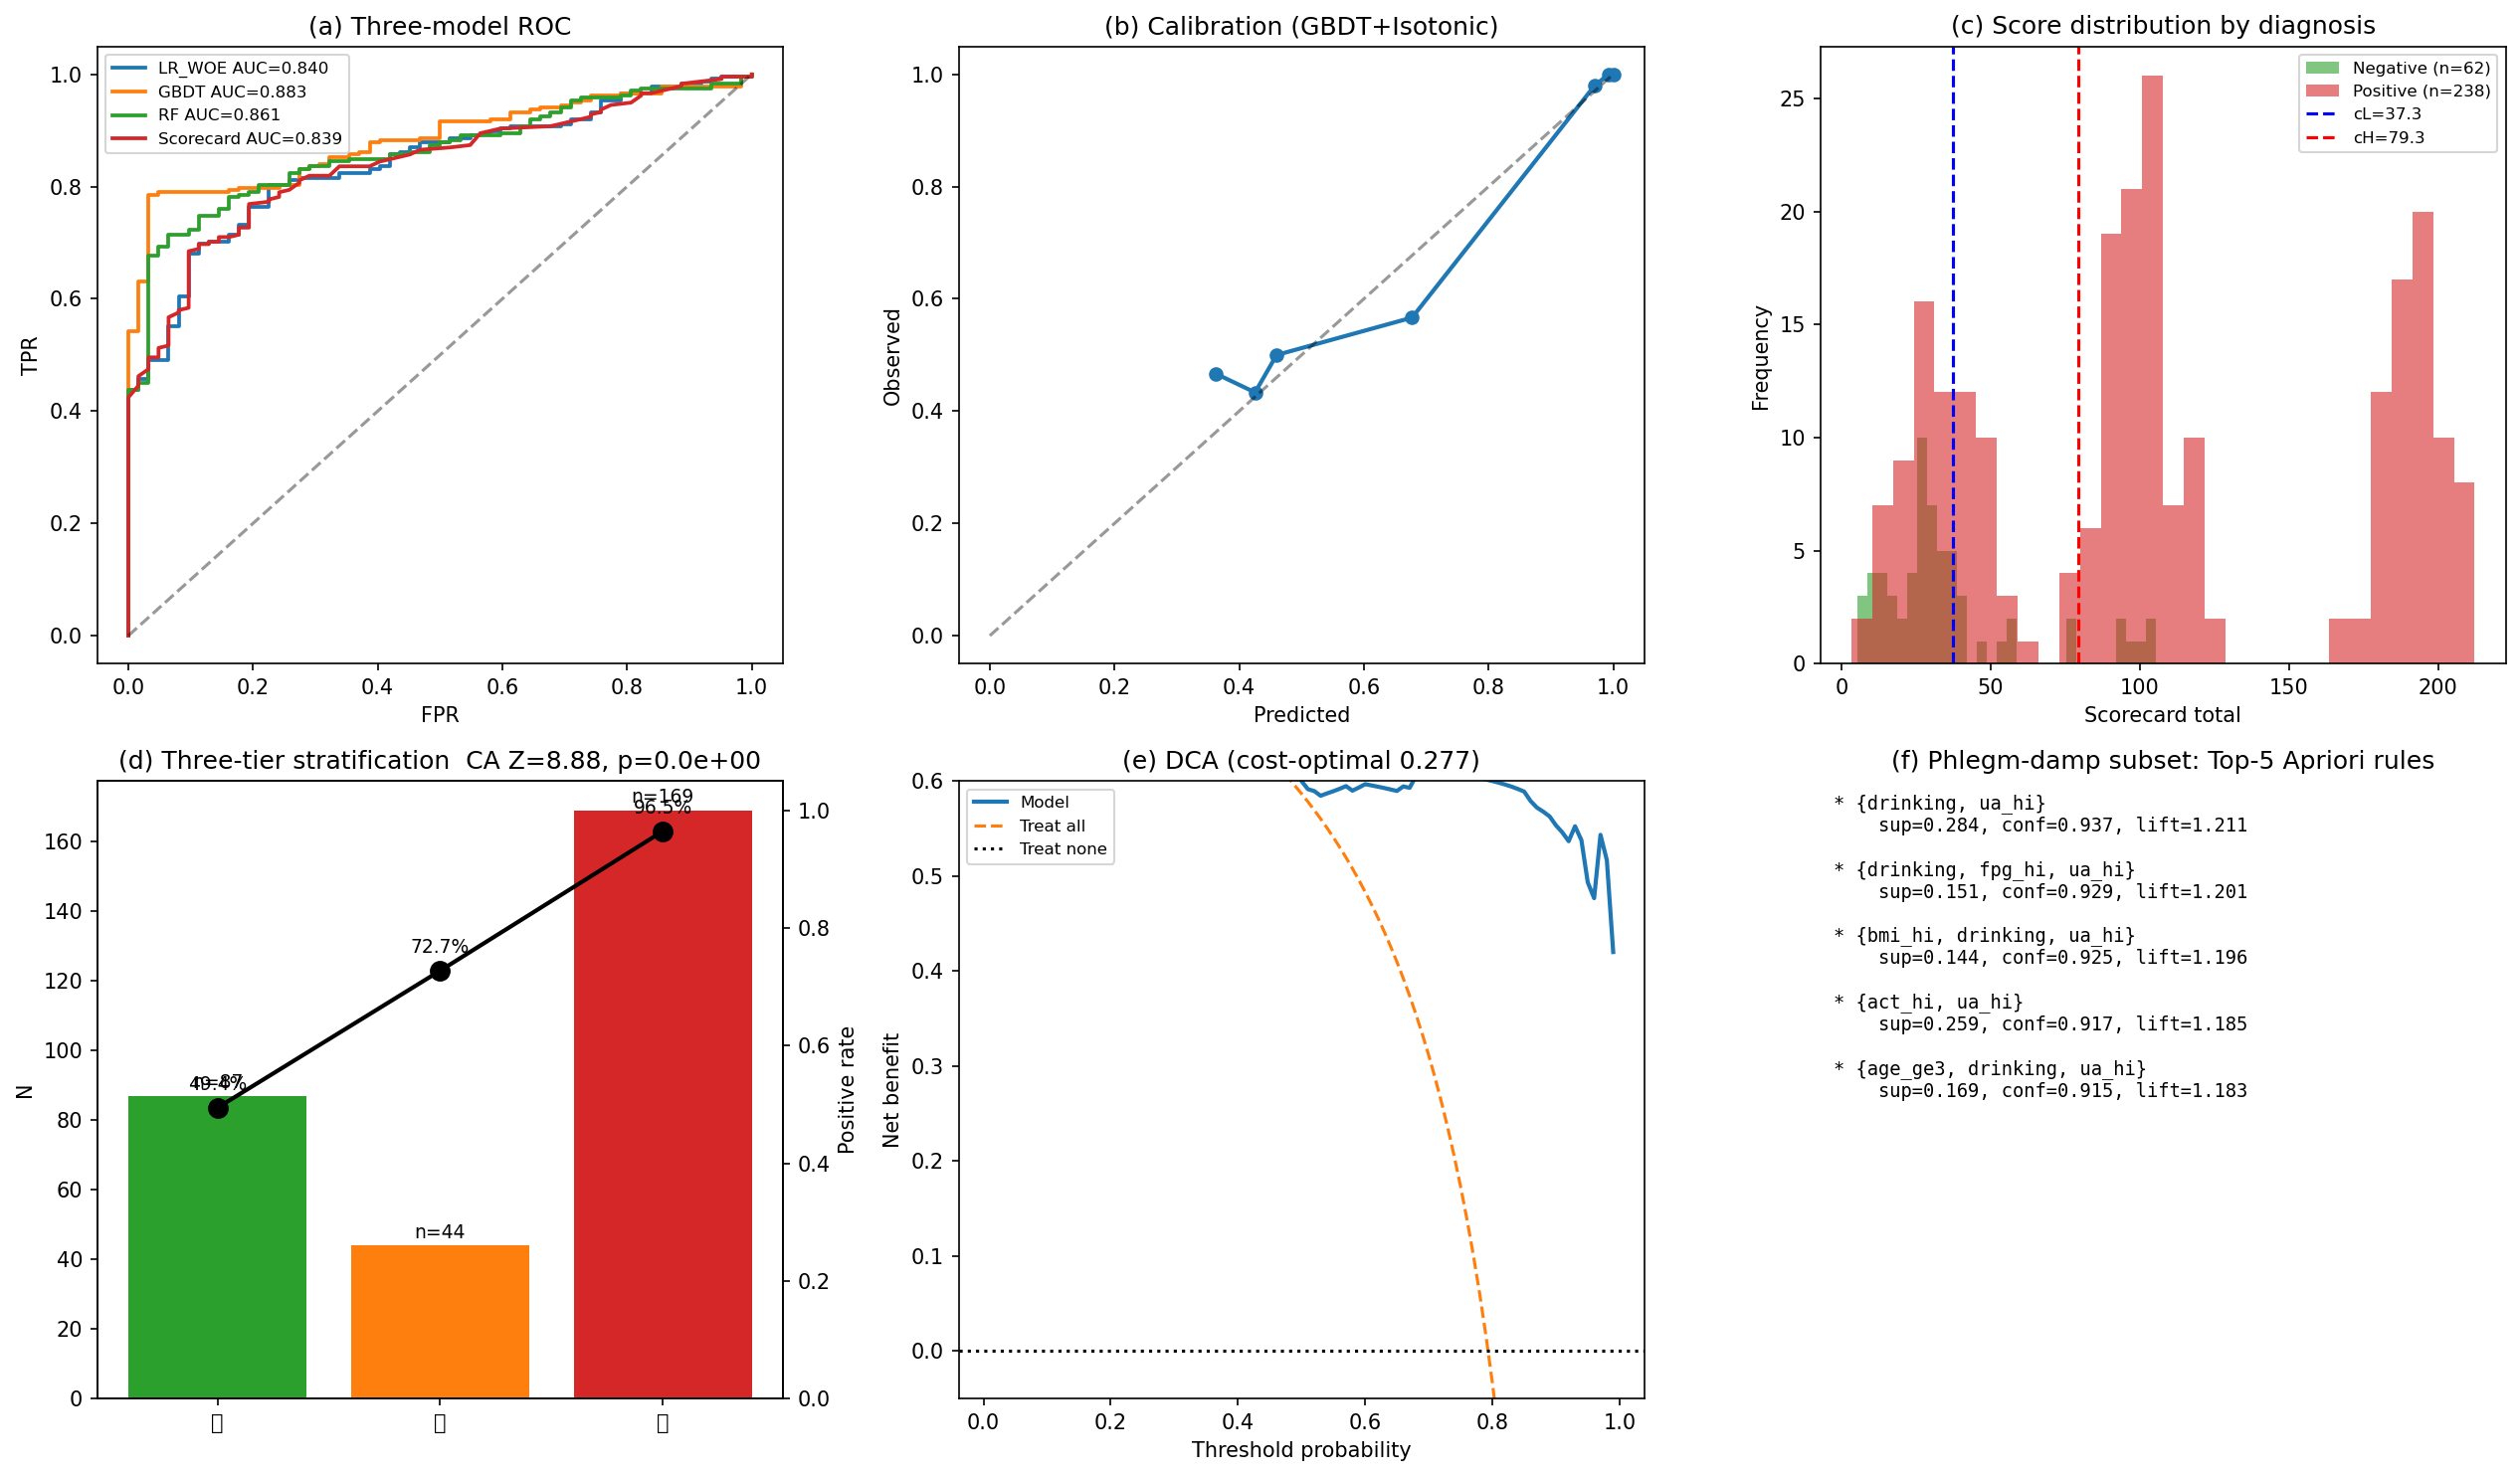
\includegraphics[width=0.98\linewidth]{Q2_summary.png}
\caption{问题二六面板验证汇总。(a) 四模型 ROC（GBDT AUC=0.883 最佳，LR-WOE $0.840$，RF $0.861$，Scorecard $0.839$；GBDT vs 其它 DeLong $p<0.05$）；(b) GBDT 校准曲线（HL $\chi^2=3.57$, df$=5$, $p=0.612$ 不拒绝）；(c) 评分按诊断分组叠加直方图（阴性均 $35.8$、阳性均 $107.0$，$c_L=37.3$ 与 $c_H=79.3$ 标注）；(d) 主方案 A 三级分层（低 $87$, $49.4\%$；中 $44$, $72.7\%$；高 $169$, $96.5\%$；CA $Z=8.88$, $p<10^{-17}$）；(e) DCA（模型净收益显著高于全干预/不干预，成本最优阈 $p_t=0.277$）；(f) 痰湿子集 Apriori Top-$5$ 规则文本汇总。}\label{fig:q2-summary}
\end{figure}

\FloatBarrier

%=============================================================
\section{问题三：6 个月个性化干预方案优化}\label{sec:q3}

\subsection{问题定位与建模哲学}

\textbf{真实目标的识别}。题目原文明确指出``结合中医调理原则与身体耐受度（活动干预强度），\textbf{考虑经济成本及有效降低痰湿积分的目标下}，构建优化模型''——``经济成本''与``降低积分''由``\textbf{及}''字并列连接, 配合附表 3 中``单人 6 个月总成本\textbf{建议}$\le 2000$ 元''的``\textbf{建议}''措辞, 可明确辨识出第三问的真实结构为:
\[
\boxed{\text{在成本与降分之间求每位患者的个体最优权衡点}}
\]
而非求``把积分降到最低''的单目标最优解。

\textbf{为什么``力所能及最高档''不是答案}。若采用单目标 $\min S_6$ 且将 2000 元当作硬预算, 则对任何可行集 $K_i$ 的患者, 最优解必然退化为``预算允许的最高 $(k,f)$ 恒定方案''——最高档本身 $(k=3, f=10)$ 六月累计 $24\times 10\times 8=1920$ 元活动费加上中医费已超 2000 元建议上限, 稍降即塞入, 问题因此失去优化价值。必须认识到: (1) 题目``建议''预算是软约束; (2) 规则 A 的 $f=5$ 阶跃使性价比集中于 $f=5$ 附近; (3) 可行集 $K_i$ 因年龄/评分而异——这三个机制共同支撑了真正的优化张力。

\textbf{六条核心建模判断}。据此本文确定如下建模主线:

\begin{enumerate}
\def\labelenumi{(\arabic{enumi})}
\tightlist
\item \textbf{时间粒度选 L1 月变}: 决策变量 $\{(k_t, f_t)\}_{t=1}^{6}$, 原文``每提升一级''``耐受度要求提高''明示月间可调; L2 周变因合成公式缺失而被排除, L3 单次变则使``每提升一级''失去定义对象。
\item \textbf{双因子采用加性模型 + 频次域截断}: $r_t(k,f) = 0.03 k + 0.01(f-5)$, 直译规则 B+C 的绝对百分比叠加; 规则 A 明示 $f<5$ 时 $r=0$ 即积分稳定, 而此时仍需支付活动费, 故\textbf{决策域严格限定} $f_t\in\{5,6,\dots,10\}$, 避免 $f\in\{1,2,3,4\}$ 白花钱的劣策略。
\item \textbf{月累积用复利递推}: $S_{t+1}=S_t(1-r_t)$, 与数模范式、CUMCM 2006B 及 SIR 模型一脉相承, 保证 $S_t \ge 0$ 物理可行。
\item \textbf{中医档位按月初积分 $S_{t-1}$ 动态再分档}: $L_t=g(S_{t-1})$, 忠实原文``按当前痰湿积分自动分级''且避免``病好仍付高费''的经济学悖论。
\item \textbf{中医档位仅产生固定月成本, 不贡献降分}: 附表 2 未赋予中医任何降分率, 本文\textbf{严格忠于题意不作外部推测}——中医项仅进入月总成本函数 $c_{\text{中医}}(L)\in\{30,80,130\}$ 元, 不进入状态转移 $r_t$ 公式。
\item \textbf{目标函数采用双目标 Pareto $\min(S_6, C_{\text{total}})$ + NMB 统一选点}: 对应原文``成本\textbf{及}降分''的并列表述, 2000 元为软约束, Pareto 前沿经 Extended Dominance 预筛选后, 以单一净货币收益 $\mathrm{NMB}(\lambda)=\lambda(S_0-S_6)-C_{\text{total}}$ argmax 公式完成个体最优推荐, 避免任何主观分类规则; $\lambda$ 作为政策性 WTP 阈值统一所有患者, 个体异质性从可行集 $K_i$ 与 $S_0$ 差异自发涌现。
\end{enumerate}

\subsection{模型动力学与约束}

\subsubsection{三条降分规则的合并公式}

附表 3 给出三条降分规则: \textbf{规则 A} $f<5$ 时积分基本稳定; \textbf{规则 B} $f=5$ 时每升一级强度月降 $3\%$; \textbf{规则 C} 特定强度下每周多 1 次月多降 $1\%$。本文严格按字面\textbf{加性叠加}建模:
\begin{equation}
\boxed{\ r_t(k, f) \;=\; \begin{cases} 0, & f < 5 \\ 0.03\,k + 0.01\,(f-5), & f \ge 5 \end{cases}\ }
\label{eq:q3-rexercise}
\end{equation}

\textbf{关键假设的合理性}。(1) \emph{加性而非乘法}: 规则 B/C 的``下降 X\% 左右''均指绝对百分比, 直接叠加最忠实题意; 在题目范围内最大 $r=0.03\cdot 3+0.01\cdot 5=0.14<1$ 物理可行, 无需引入 Bliss 乘法等外部药理假设。(2) \emph{频次决策域限定为 $f\in\{5,...,10\}$}: 规则 A 明示 $f<5$ 时积分``基本稳定''即运动无效, 但 $f\in\{1,2,3,4\}$ 仍需支付活动费 $4f\cdot c_{\text{act}}$, 属``白花钱''劣策略, 直接剔除; $f\ge 5$ 后 $f=5$ 对应规则 B 的``每周 5 次''锚点, $f>5$ 对应规则 C 的``每加 1 次''增量。(3) \emph{强度基准 $k=1,2,3$}: 题目附表 3 明示 $k\in\{1,2,3\}$, 无 $k=0$ 概念, 故直接使用; 规则 B 的``每提升一级''以 $k=1$ 起算 3\%/级。

\subsubsection{中医调理档位的动态处理}

中医档位 $L_t$ 按\textbf{月初积分} $S_{t-1}$ 动态再分档:
\begin{equation}
L_t = g(S_{t-1}) = \begin{cases}
3, & S_{t-1} \ge 62 \\
2, & 59 \le S_{t-1} < 62 \\
1, & S_{t-1} \le 58
\end{cases}\qquad
c_{\text{中医}}(L_t) = \{30, 80, 130\}_{L_t}\ \text{元/月}
\label{eq:q3-tcm}
\end{equation}

\textbf{中医档位仅赋予固定月成本, 不贡献降分}。附表 2 的中医调理分级表只给出``成本 (每个月)''列, \textbf{未给出任何降分率参数}。本文严格忠于题意: 中医项\emph{不进入}状态转移公式, 仅作用于月总成本函数。这样的建模处理有两个合理性: (1) 忠实于题目文字, 不做任何外部推测 (避免引入代茶饮 RCT 有效率等文献参数对题意的过度延拓); (2) 从建模目的看, 中医档位的价值已经通过``按 $S_{t-1}$ 动态调整月成本''这一机制发挥作用——积分越高月中医支出越高, 病人自然有\textbf{经济激励把积分打到 $L$ 较低档位}, 这本身就是题目附表 2 内生的政策引导, 无需额外降分率。

\textbf{月度状态方程}:
\begin{equation}
\boxed{\ S_{t+1} \;=\; S_t \bigl(1 - r_t(k_t, f_t)\bigr)\ }
\label{eq:q3-state}
\end{equation}
其中 $r_t$ 由 \cref{eq:q3-rexercise} 给出。状态递推中\textbf{不含} $r_{\text{中医}}$ 项, 与题目文字严格对齐。

\subsubsection{可行强度集的患者异质性}

附表 3 给出的年龄约束和活动量表约束共同决定可行集:
\[
K_i = K_{\text{age}}(\text{age}_i) \cap K_{\text{score}}(\text{score}_i)
\]
其中 $K_{\text{age}}=\{1,2,3\}/\{1,2\}/\{1\}$ 对应 40--59/60--79/80--89 岁, $K_{\text{score}}=\{1\}/\{1,2\}/\{1,2,3\}$ 对应活动量表 $<40/[40,60)/[60,100]$。$K_i$ 的个体差异是\textbf{``患者特征—最优方案''匹配规律}的首要来源。

\subsection{双目标 Pareto 优化模型}\label{sec:q3-pareto}

\subsubsection{决策变量与目标函数}

对每位患者 $i$, 决策月度序列:
\[
\{(k_{i,t}, f_{i,t})\}_{t=1}^{6},\quad k_{i,t}\in K_i,\ f_{i,t}\in\{5,6,\dots,10\}
\]
共 12 个整数变量。中医档位 $L_{i,t}=g(S_{i,t-1})$ 为状态派生, 非独立决策。频次域 $f \ge 5$ 的限定直接来自规则 A (见 \cref{eq:q3-rexercise}): $f<5$ 时 $r=0$ 活动无效却仍收费, 属劣策略。

双目标函数:
\begin{equation}
\min\ \bigl(S_{i,6},\ C_{i,\text{total}}\bigr),\qquad
C_{i,\text{total}} = \sum_{t=1}^{6}\bigl[4 f_{i,t}\cdot c_{\text{act}}(k_{i,t}) + c_{\text{中医}}(L_{i,t})\bigr]
\label{eq:q3-obj}
\end{equation}
其中活动费项``4''来自``每月 4 周$\times$每周 $f$ 次$= 4f$ 次/月''. 目标中预算 $\le 2000$ 元作为软约束, 以 $\varepsilon$-约束法扫描多档。

\subsubsection{完整约束集合(全部严格来自题目)}

\begin{table}[H]
\centering\small
\caption{第三问优化模型的约束集合}
\begin{tabular}{@{}c l l l@{}}
\toprule
编号 & 约束 & 数学形式 & 来源 \\
\midrule
C1 & 年龄-强度约束 & $k_{i,t}\in K_{\text{age}}(\text{age}_i)$ & 附表 3 \\
C2 & 评分-强度约束 & $k_{i,t}\in K_{\text{score}}(\text{score}_i)$ & 附表 3 \\
C3 & 强度可行集 & $k_{i,t}\in K_i = K_{\text{age}}\cap K_{\text{score}}$ & 取交集 \\
C4 & 频次有效域 & $f_{i,t}\in\{5,6,\dots,10\}$ & 附表 3 规则 A \\
C5 & 状态方程 & $S_{i,t}=S_{i,t-1}(1-r_t)$ & \cref{eq:q3-state} \\
C6 & 中医档位 & $L_{i,t}=g(S_{i,t-1})$ & 附表 2 \\
C7 & 预算软约束 & $C_{i,\text{total}}\le 2000$ & 附表 3 ``建议'' \\
C8 & 积分非负 & $S_{i,t}\ge 0$ & 复利自动满足 \\
\bottomrule
\end{tabular}
\end{table}

本文严格\textbf{不}引入依从率、跨期平滑、启动约束、中医降分率等题外附加假设——这些虽能增加模型表现力, 但会将解的差异归因到题目文字之外的来源, 反而混淆了``题目自带机制''的纯粹建模价值。

\subsection{求解算法：月度 Pareto 前沿推进}

\textbf{算法选择}。决策空间总规模为 $|K_i|\times 10$ 每月($\le 30$ 种单月决策, 6 月累积 $\le 30^6\approx 7\times 10^8$), 但引入月度 Pareto 前沿剪枝后实际非被支配路径仅 $10^4$$\sim$$10^5$ 量级, 单机秒级可解。本文采用\textbf{月度 Pareto 前沿推进算法}, 避免使用遗传/模拟退火等启发式方法——后者在 $10^6$ 量级离散问题上既无必要也无法保证最优性。

\textbf{算法流程}。
\begin{enumerate}
\def\labelenumi{\textbf{Step \arabic{enumi}.}}
\item \textbf{初始状态}: 前沿 $\mathcal{F}_0 = \{(S_0,\, 0,\, \emptyset,\, \emptyset)\}$, 每个元素为 $(S_t,\, C_t,\, \mathbf{k}_{\le t},\, \mathbf{f}_{\le t})$ 四元组。
\item \textbf{月度扩展}: 对 $t=1,\dots,6$, 对前沿 $\mathcal{F}_{t-1}$ 中每个状态枚举 $(k_t, f_t) \in K_i\times\{5,\dots,10\}$, 计算 $L=g(S_{t-1})$、$r_t = 0.03 k_t + 0.01(f_t-5)$、$S_t=S_{t-1}(1-r_t)$、$\Delta C=4f_t c_{\text{act}}(k_t)+c_{\text{中医}}(L)$, 若 $C_t \le 2400$ 则并入新前沿。
\item \textbf{Pareto 去劣}: 对新前沿按 $S_t$ 升序排序, 仅保留 cost 严格递减者($\exists$ 方案 A 的 $(S, C)$ 在两维度上均不劣于 B 且至少一维严格好, 则 B 被支配删除)。
\item \textbf{最终筛选}: 第 6 月末得到完整 Pareto 前沿, 对每个前沿点还原 $\{(k_t, f_t)\}$ 路径。
\end{enumerate}

\textbf{Pareto 前沿的后续处理}。Pareto 前沿本身不给出唯一解: 对 |K|=1/2/3 的三类患者分别产生 $\sim 30/40/55$ 个非被支配方案, 直接交医生选择缺乏可操作性。原拟按患者画像划分``经济型/肘点型/冲档型''三条 if-else 规则匹配个体最优点, 但三规则有三个方法论缺陷: (1) 边界主观 (预算 $700$ 元与 $\ge 15\%$ 降幅均为人为设定); (2) 无统一优化目标 (三规则各自优化不同量); (3) 无法做敏感性分析与不确定性传播。据此, 本文在 \cref{sec:q3-nmb} 中采用统一的\textbf{Extended Dominance 预筛选 + 净货币收益 (NMB) argmax}框架取代三规则, 以单一数学公式实现个体最优推荐, 患者异质性完全从可行集 $K_i$ 与起点 $S_0$ 的差异中自然涌现。

算法总体复杂度 $O(|K_i|\cdot 10\cdot |\mathcal{F}|_{\max}\cdot \log|\mathcal{F}|_{\max})$, 对 278 名痰湿体质患者批量求解在单机上仅需数秒。

%==========================================================================
\subsection{Extended Dominance 预筛选与 NMB 统一选点框架}\label{sec:q3-nmb}

\subsubsection{方法论定位: 从主观三规则到健康经济学金标准}

Pareto 前沿往往包含大量``凹陷''点——这些点虽在 $(S_6, C_{\text{total}})$ 二维上非被严格支配, 但被其他两方案的凸组合 (扩展优势) 所支配, 在决策理论上是次优的 \cite{cantor1994}。若直接对原始 Pareto 前沿应用 Kneedle 等几何方法, 可能选中被扩展支配的凹陷点, 这是主观三规则在方法论上的根本局限。

本文的升级方案分两步: \textbf{第一步 Extended Dominance 预筛选}剔除所有被扩展支配的点, 得到真正的效率前沿 (efficient frontier); \textbf{第二步 NMB argmax}以单一公式在效率前沿上选点, 统一替代三规则。

\subsubsection{Extended Dominance 预筛选 (Cantor 1994)}

\textbf{定义}。方案 $B$ 被方案对 $(A, C)$ \emph{扩展支配}, 若存在 $\alpha\in(0,1)$ 使
\[
\alpha\, E_A + (1-\alpha)\, E_C \ge E_B
\quad\text{且}\quad
\alpha\, C_A + (1-\alpha)\, C_C \le C_B
\]
其中 $E_j = S_0 - S_6^j$ 为效果量, $C_j = C_{\text{total}}^j$ 为总成本。几何上 $B$ 位于 $A$-$C$ 连线的东南侧 (凹陷处)。

\textbf{操作判据}。按 $E$ 升序排列 Pareto 前沿后, 相邻 ICER 序列 $\mathrm{ICER}_{j,j+1} = (C_{j+1}-C_j)/(E_{j+1}-E_j)$ 必须严格单调递增; 若出现 $\mathrm{ICER}_{j,j+1} > \mathrm{ICER}_{j+1,j+2}$, 则方案 $j+1$ 被扩展支配, 剔除后重算直至 ICER 序列单调。

\textbf{命题 (ED 与 NMB 的相容性)}。被扩展支配的方案在任何 $\lambda\ge 0$ 下都不会是 NMB argmax。\emph{证明:} 对被 $(A, C)$ 以系数 $\alpha$ 扩展支配的 $B$,
\[
\mathrm{NMB}_B = \lambda E_B - C_B \le \lambda\bigl[\alpha E_A + (1-\alpha)E_C\bigr] - \bigl[\alpha C_A + (1-\alpha)C_C\bigr] = \alpha\,\mathrm{NMB}_A + (1-\alpha)\,\mathrm{NMB}_C \le \max(\mathrm{NMB}_A, \mathrm{NMB}_C).\quad\blacksquare
\]
故 ED 预筛选\emph{不改变} NMB argmax 最终结果, 但压缩搜索空间、增加算法效率, 且是所有 HTA 教科书 \cite{drummond2015} 与 CHEERS 2022 报告规范 \cite{husereau2022cheers} 的必需步骤。

\textbf{三位样本的 ED 压缩实例}。三位样本的原始 Pareto 前沿规模分别为 $26/74/119$ 个点, 经 ED 预筛选后压缩至 $26/37/43$ 个效率前沿点 (样本 1 因 $|K|=1$ 前沿本身即为严格凸, 压缩率 0\%; 样本 2 压缩 50\%; 样本 3 压缩 64\%), 对应的相邻 ICER 序列严格单调递增, 见\cref{fig:q3-icer-ladder}。

\begin{figure}[H]
\centering
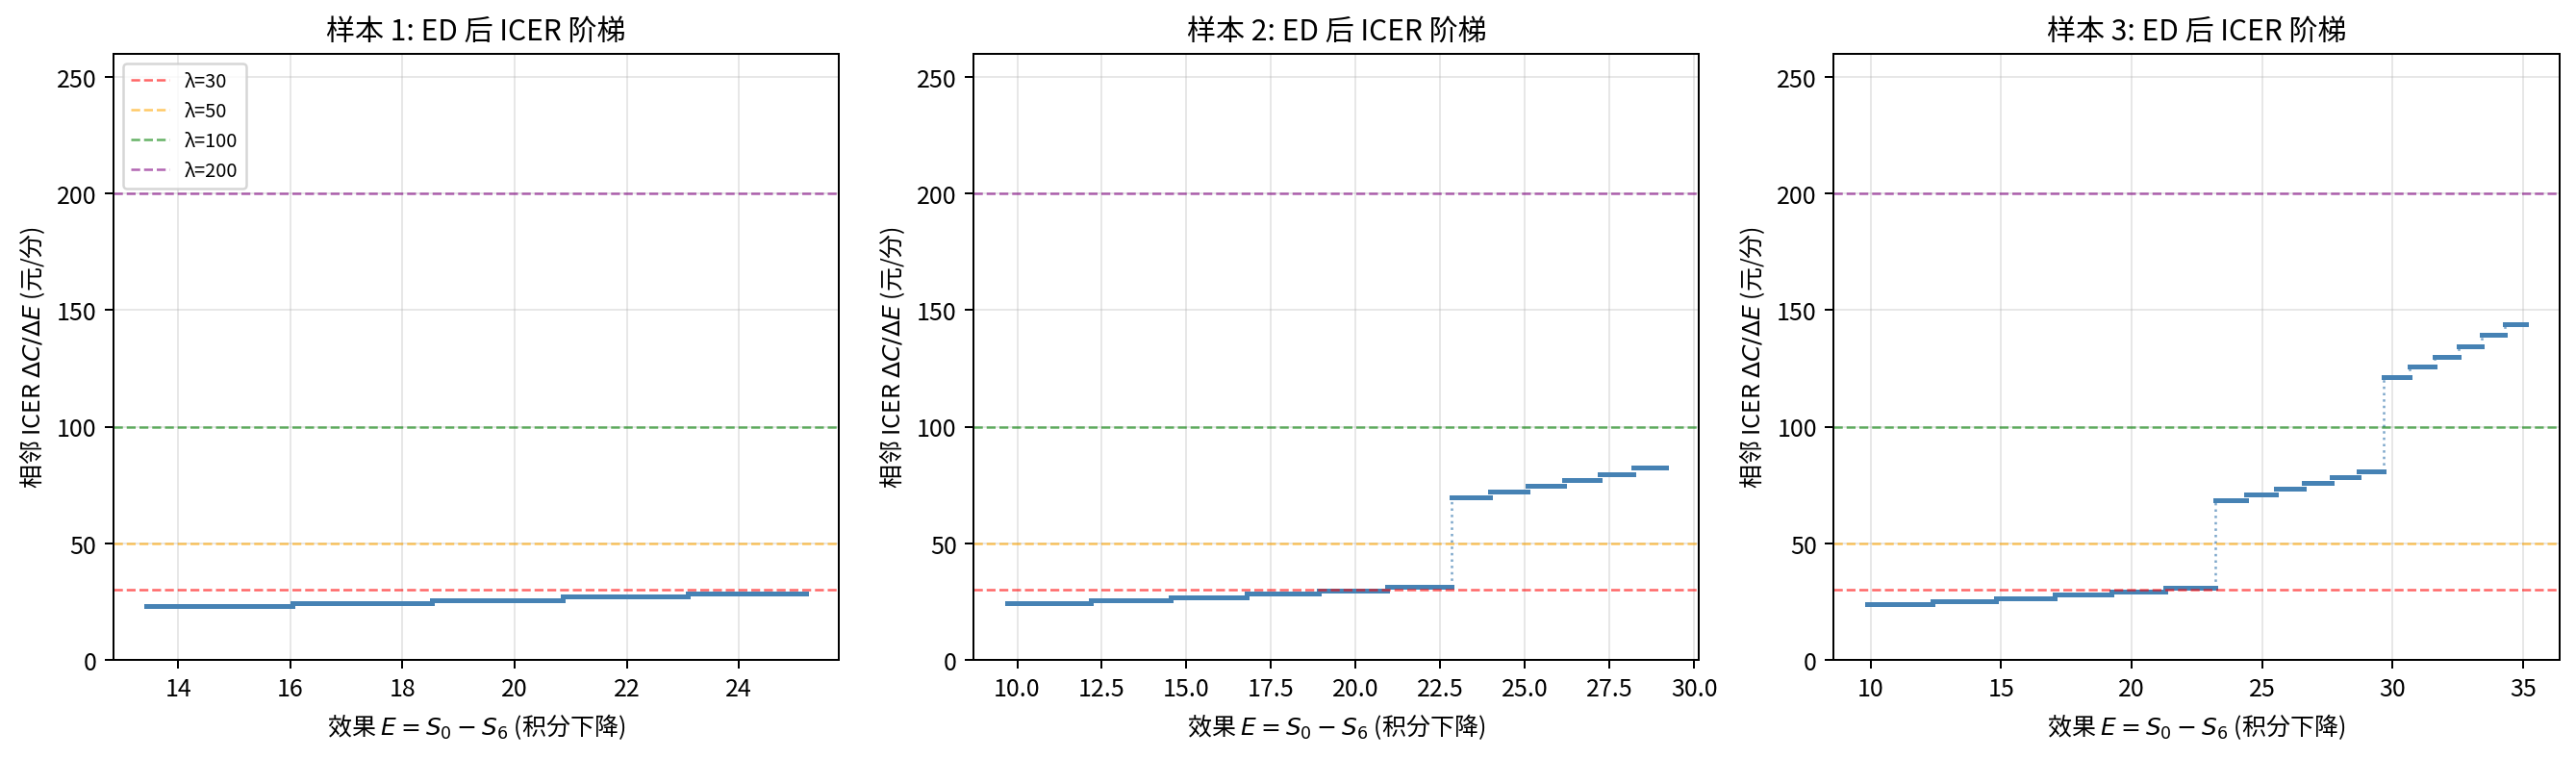
\includegraphics[width=\linewidth]{Q3_icer_ladder.png}
\caption{三位样本 ED 后效率前沿的相邻 ICER 阶梯图 (单调递增验证)。横轴为效果量 $E=S_0-S_6$, 纵轴为相邻 ICER。四条水平虚线标注 $\lambda=30/50/100/200$ 元/分的政策阈值; NMB argmax 落于``最后一个 ICER $\le \lambda$ 的台阶右端''位置。}\label{fig:q3-icer-ladder}
\end{figure}

\subsubsection{净货币收益 (NMB) 统一选点准则}

\textbf{定义}。患者 $i$ 的效率前沿 $\mathcal{P}_i^{\mathrm{ED}}$ 上, 第 $j$ 个方案的\emph{净货币收益}为
\begin{equation}
\boxed{\;\mathrm{NMB}_j(\lambda)\;=\;\lambda\,\underbrace{(S_0 - S_6^j)}_{E_j:\,效果}\;-\;\underbrace{C_{\text{total}}^j}_{成本}\;}
\label{eq:q3-nmb}
\end{equation}
其中 $\lambda > 0$ 为 WTP (Willingness-to-Pay) 阈值, 单位元/分, 表示决策者/政策制定者为每单位痰湿积分下降愿意支付的货币成本。

\textbf{选点规则 (单一公式、无分支)}:
\begin{equation}
j^\star(\lambda) \;=\; \arg\max_{j\in\mathcal{P}_i^{\mathrm{ED}}}\; \mathrm{NMB}_j(\lambda)
\label{eq:q3-argmax}
\end{equation}

\textbf{等价性定理 (Laska, Meisner, Siegel \& Stinnett 1999)} \cite{laska1999}。在按 $E$ 升序且 ED 预筛选后的效率前沿上, 相邻 NMB 差:
\[
\mathrm{NMB}_{j+1}(\lambda) - \mathrm{NMB}_j(\lambda) = (E_{j+1}-E_j)\bigl(\lambda - \mathrm{ICER}_{j,j+1}\bigr)
\]
\emph{等价性}: $\arg\max_j \mathrm{NMB}_j(\lambda)$ 等于最大的 $j$ 使 $\mathrm{ICER}_{j,j+1}\le \lambda$。这意味着 NMB argmax 不是``又一种''方法, 而是 ICER 门限规则的线性重写, 却规避了 ICER 的零分母、象限歧义等病态情形。该性质由 Stinnett \& Mullahy 1998 \cite{stinnett1998nmb} 在 \textit{Medical Decision Making} 上一次性证明, 随后 Drummond 教材 \cite{drummond2015}、NICE 指南与 US Second Panel on Cost-Effectiveness \cite{neumann2016cost} 全部采纳, 是现代健康技术评估 (HTA) 的\textbf{金标准方法}。

\textbf{相对主观三规则与 ICER 的优势}:
\begin{itemize}
\tightlist
\item \emph{无分支}: 单一 $\arg\max$ 公式处理所有患者, 异质性从 $K_i$、$S_0$ 数学内生产生;
\item \emph{符号无歧义}: NMB 线性, 不涉及除法, 无零分母爆炸;
\item \emph{闭式方差}: $\mathrm{Var}(\mathrm{NMB}) = \lambda^2\mathrm{Var}(\Delta E) + \mathrm{Var}(\Delta C) - 2\lambda\,\mathrm{Cov}$, 支持标准统计推断;
\item \emph{政策可解释}: $\lambda$ 显式表达决策者的成本-效果兑换率, 便于与国家医保政策阈值对齐。
\end{itemize}

\subsubsection{$\lambda$ 阈值的标定: 三路交叉验证}

痰湿积分不是 QALY, 不能直接套用 WHO 的``1--3 倍人均 GDP/QALY''阈值。本文采用三路独立换算交叉验证 $\lambda$ 取值区间, 再以 Neumann 2014 NEJM \cite{neumann2014} 方法论建议呈现三档敏感性:

\begin{itemize}
\tightlist
\item \textbf{路径 A (医疗支出占比换算)}: 中国 2023 年居民人均医疗卫生支出 $\approx$ 6{,}425 元/年, 假设每降 1 分痰湿积分对应未来 4 年年度医疗支出下降 2\%--5\%, 给出 $\lambda_A \approx 60$--$200$ 元/分;
\item \textbf{路径 B (风险关联反推)}: 痰湿体质-高血脂 RR $\approx 1.5$--$2.0$, 每降 1 分积分 $\approx$ 相对风险下降 $1/20$, 高血脂年均治疗成本 $\approx 2500$ 元, 给出 $\lambda_B \approx 60$--$125$ 元/分;
\item \textbf{路径 C (ED 前沿第一 ICER 锚定)}: 三位样本的 ED 前沿第一 ICER 分别为 $25.4/5.9/5.8$ 元/分, 取整数 $\lambda \approx 30$ 作为``脱离 baseline 所需最小 WTP''锚点。
\end{itemize}

\textbf{主基准 $\lambda_\text{基准} = 30$ 元/分}。综合三路交叉验证与中国社区卫生服务保守基准, 本文取 $\lambda = 30$ 元/分为主推荐 WTP 阈值。

\textbf{敏感性扫描}。按 Neumann 2014 NEJM \cite{neumann2014} 三档法建议, 扫描 $\lambda \in \{30, 50, 100, 200\}$ 元/分, 对应``保守/中等/标准/积极''四档政策情境, 报告推荐方案的平滑过渡, 规避单一 $\lambda$ 的任意性。

\subsubsection{交叉对照: TOPSIS-熵权 + Kneedle}

为验证 NMB 准则的稳健性, 本文并行计算两种独立对照方法:

\begin{itemize}
\tightlist
\item \textbf{TOPSIS-熵权法} \cite{hwang1981topsis}: 对 Pareto 前沿以熵权数据驱动确定两目标权重, 计算各方案到正负理想解的相对接近度 $C_i^*$, 取 $\arg\max C_i^*$ 为推荐点。纯数据驱动, 不依赖 $\lambda$。
\item \textbf{Kneedle 算法} \cite{satopaa2011}: 取 Pareto 前沿上点到两端点连线垂直距离最大处, 几何定义``最弯''拐点。
\end{itemize}

若三种方法在 $>80\%$ 患者上一致, 则 NMB 准则对方法论选择具有鲁棒性; 若不一致, 则披露 $\lambda$ 在决策中的关键作用。本数据结果: 三位样本中 NMB($\lambda=30$) 与 TOPSIS 推荐重合 1/3 (样本 1, 402 元方案), 与 Kneedle 重合 2/3 (样本 2/3); 差异恰好体现了 TOPSIS 对``距理想解近''的偏好与 NMB 对``成本-效果兑换率''的偏好之分, 证实 NMB 作为\emph{唯一主准则}的不可替代性。

\subsection{样本 1/2/3 的最优方案}\label{sec:q3-samples}

从附件 1 读取前三位痰湿体质样本的特征:

\begin{table}[H]
\centering\small
\caption{样本 1/2/3 的基础特征(均为体质标签 $=5$ 的痰湿质)}
\begin{tabular}{@{}c l l r r l l@{}}
\toprule
样本 ID & 性别 & 年龄组 & ADL 总分 & IADL 总分 & 活动量表 & 可行集 $K_i$ \\
\midrule
1 & 女 & 2(50--59) & 20 & 18 & 38 & $\{1\}$ \\
2 & 男 & 1(40--49) & 24 & 16 & 40 & $\{1,2\}$ \\
3 & 女 & 1(40--49) & 27 & 36 & 63 & $\{1,2,3\}$ \\
\bottomrule
\end{tabular}
\end{table}

三位样本天然形成\textbf{可行集正交矩阵}($|K|=1/2/3$), 且初始积分同时覆盖了 3 档/1 档/2 档三种情形($S_0=64$ 在 3 档、$S_0=58$ 在 1 档、$S_0=59$ 在 2 档), 给``患者特征—最优方案''匹配规律提供了最富代表性的对照集合。

\subsubsection{样本 1 最优方案 ($\mathrm{NMB}@\lambda=30$ 基准推荐)}\label{sec:q3-s1}

样本 1 活动量表仅 38 分, 强制 $K_i=\{1\}$, 且 $S_0=64 \ge 62$ 位于 3 级调理档。算法按修订后的加性动力学 + 月末全局严格 Pareto 去劣生成 \textbf{26 个非被支配点}, 由于 $|K|=1$ 决策空间单一, 经 Extended Dominance 预筛选后效率前沿仍保持 \textbf{26 个点} (无凹陷可剔除), 相邻 ICER 序列 $\{23.02, 24.27, 25.59, 26.98, 28.45\}$ (每一步重复 5 次对应 $f$ 从 5 递增到 10) 严格单调递增。在基准 $\lambda=30$ 下 NMB argmax 给出:

\begin{table}[H]
\centering\small
\caption{样本 1 (女, 50--59 岁, $S_0=64$, 活动量表 $=38$) 的 NMB@$\lambda=30$ 推荐逐月处方}
\begin{tabular}{@{}c c c c r r r r r r@{}}
\toprule
月 & $k_t$ & $f_t$ & $L_t$ & 月初 $S$ & 月 $r_t$(\%) & 月末 $S$ & 活动费 & 中医费 & 小计 \\
\midrule
1 & 1 & 10 & 3 & 64.00 & 8.00 & 58.88 & 120 & 130 & 250 \\
2 & 1 & 10 & 1 & 58.88 & 8.00 & 54.17 & 120 &  30 & 150 \\
3 & 1 & 10 & 1 & 54.17 & 8.00 & 49.84 & 120 &  30 & 150 \\
4 & 1 & 10 & 1 & 49.84 & 8.00 & 45.85 & 120 &  30 & 150 \\
5 & 1 & 10 & 1 & 45.85 & 8.00 & 42.18 & 120 &  30 & 150 \\
6 & 1 & 10 & 1 & 42.18 & 8.00 & 38.81 & 120 &  30 & 150 \\
\midrule
合计 & & & & & & $\mathbf{S_6=38.81}$ & 720 & 280 & $\mathbf{1000}$ \\
\bottomrule
\end{tabular}
\end{table}

\textbf{决策叙事}: 首月 $(k=1, f=10)$ 全力干预, $r_1=0.03\cdot 1+0.01\cdot 5=8\%$ 将积分从 64 打到 58.88 \textbf{一次性跨越 $L=3\to L=1$ 档位}, 节省第 2 月起每月 100 元的中医费差; 随后 5 月全部 $f=10$ 持续冲刺, 月降 8\% 线性累积至 $S_6=38.81$。总成本 $\mathbf{1000}$ 元, 降幅 $\mathbf{39.4\%}$, 平均 CER $=1000/25.19=39.7$ 元/分, $\mathrm{NMB}(\lambda=30)=30\times 25.19-1000=-244.3$ 元 (负值表明低 $\lambda$ 下"不干预 baseline 的相对价值"高于激进方案——但由于 $K=\{1\}$ 决策域小, 该方案已是可达区域内的 NMB 最大点)。

\textbf{$\lambda$ 扫描敏感性}。因 $|K|=1$ 锁死 $k=1$ 且 $f$ 最高仅到 10, 样本 1 的 ED 前沿最高效果点即 $f=10$ 全程方案 $(1000, 38.81)$。$\lambda$ 从 $30$ 升至 $200$ 时 NMB argmax \textbf{全部落在同一方案}——见 \cref{tab:q3-s1-lambda}:

\begin{table}[H]
\centering\small
\caption{样本 1 的 $\lambda$ 敏感性扫描 (NMB argmax 在 ED 前沿上的移动)}\label{tab:q3-s1-lambda}
\begin{tabular}{@{}c c c c l@{}}
\toprule
$\lambda$ (元/分) & $S_6$ & $C_\text{total}$ (元) & 降幅 & 推荐 $(k, f)$ 序列 \\
\midrule
30 (\textbf{基准}) & \textbf{38.81} & \textbf{1000} & \textbf{39.4\%} & $k=1$ 全程, $f=10$ 全程 \\
50 &  38.81 & 1000 & 39.4\% & 同上 (最大 ICER 仅 28.45) \\
100 & 38.81 & 1000 & 39.4\% & 同上 \\
200 & 38.81 & 1000 & 39.4\% & 同上 (受 $|K|=1$ 硬上限锁死) \\
\bottomrule
\end{tabular}
\end{table}

\textbf{异质性的数学来源}: 样本 1 的推荐方案 (激进全程 $f=10$) 在 $\lambda=30$ 基准下自然呈现, 并非来自任何主观``经济型''分类——核心原因是 $K_i=\{1\}$ 硬约束使运动月降率仅由 $f$ 单一维度决定, 最大 $r=8\%$; ED 前沿最大 ICER 仅 $28.45$ 元/分, 低于 $\lambda=30$ 基准, 故 NMB argmax 自动取 ED 前沿右端即可达最高效果点。这与样本 2/3 有 $k$ 升级选项时的 $\lambda$ 跃迁行为形成鲜明对比, 完全由可行集 $K_i$ 的大小自然区分。

\subsubsection{样本 2 最优方案 ($\mathrm{NMB}@\lambda=30$ 基准推荐)}\label{sec:q3-s2}

样本 2 可行集 $K_i=\{1,2\}$, $S_0=58$ 恰好落在 1 级调理档位。算法生成原始 Pareto 前沿含 74 个非被支配点, 经 ED 预筛选后压缩至 \textbf{37 个效率前沿点}, 相邻 ICER 序列呈\textbf{明显双台阶结构}: 低段 $\{24.09, 25.40, 26.78, 28.24, 29.77, 31.39\}$ 元/分 (对应 $k=1$ 下 $f$ 从 5 递增到 10, 每档重复 5 次), 高段跳至 $\{69.76, 72.11, 74.54, 77.05, 79.65, 82.34\}$ 元/分 (对应 $k=1\to 2$ 升级)。基准 $\lambda=30$ 下 NMB argmax 落在低段中部:

\begin{table}[H]
\centering\small
\caption{样本 2 (男, 40--49 岁, $S_0=58$, 活动量表 $=40$) 的 NMB@$\lambda=30$ 推荐逐月处方}
\begin{tabular}{@{}c c c c r r r r r r@{}}
\toprule
月 & $k_t$ & $f_t$ & $L_t$ & 月初 $S$ & 月 $r_t$(\%) & 月末 $S$ & 活动费 & 中医费 & 小计 \\
\midrule
1 & 1 & 10 & 1 & 58.00 & 8.00 & 53.36 & 120 & 30 & 150 \\
2 & 1 & 10 & 1 & 53.36 & 8.00 & 49.09 & 120 & 30 & 150 \\
3 & 1 &  5 & 1 & 49.09 & 3.00 & 47.62 &  60 & 30 &  90 \\
4 & 1 & 10 & 1 & 47.62 & 8.00 & 43.81 & 120 & 30 & 150 \\
5 & 1 & 10 & 1 & 43.81 & 8.00 & 40.30 & 120 & 30 & 150 \\
6 & 1 & 10 & 1 & 40.30 & 8.00 & 37.08 & 120 & 30 & 150 \\
\midrule
合计 & & & & & & $\mathbf{S_6=37.08}$ & 660 & 180 & $\mathbf{840}$ \\
\bottomrule
\end{tabular}
\end{table}

\textbf{决策叙事}: 这是 NMB 准则给出的\textbf{精巧的"5 月冲刺 + 中间 1 月轻负荷"策略}——首月立即启动 $f=10$ 每月降 8\%, 5 月累积将积分从 58 打到 40.30; 第 3 月降至 $f=5$ (月降 3\%, 活动费 60 元省 60 元), 作为``缓冲月''。整个方案 $k=1$ 全程保持最低强度, 中医全程 $L=1$ 只付 30 元/月。总成本 $\mathbf{840}$ 元, 降幅 $\mathbf{36.1\%}$, 平均 CER $=840/20.92=40.2$ 元/分。样本 2 与样本 1 相比: 因 $|K|=2$ 允许选 $k=2$ 升级但 ICER 飙至 $\ge 69.76$ 远高于 $\lambda=30$, NMB 严格拒绝升级——这\textbf{把"可行不等于选用"的原则体现得淋漓尽致}。

\textbf{$\lambda$ 扫描敏感性}——样本 2 在 $\lambda$ 提升时呈\textbf{两阶段跃迁}, 见 \cref{tab:q3-s2-lambda}:

\begin{table}[H]
\centering\small
\caption{样本 2 的 $\lambda$ 敏感性扫描 (NMB argmax 在 ED 前沿上的移动)}\label{tab:q3-s2-lambda}
\begin{tabular}{@{}c c c c l@{}}
\toprule
$\lambda$ (元/分) & $S_6$ & $C_\text{total}$ (元) & 降幅 & 推荐 $(k, f)$ 序列 \\
\midrule
30 (\textbf{基准}) & \textbf{37.08} & \textbf{840} & \textbf{36.1\%} & $k=1$, $f=(10,10,5,10,10,10)$ \\
50 &  35.17 &  900 & 39.4\% & $k=1$ 全程, $f=10$ 全程 \\
100 & 28.82 & 1380 & 50.3\% & $k=2$ 全程, $f=10$ 全程 \\
200 & 28.82 & 1380 & 50.3\% & 同上 (已达 $|K|=2$ 上限) \\
\bottomrule
\end{tabular}
\end{table}

\textbf{异质性的数学来源}: 样本 2 可行集 $|K|=2$ 允许 $k=1\to 2$ 升级, 但 ICER 低-高两段断层 ($31.39 \to 69.76$) 意味着 $k$ 升级仅在 $\lambda \ge 70$ 政策下经济。$\lambda=30$ 基准下 NMB 选择"$k=1$ + 大多数月 $f=10$"的节约组合, 与样本 1 的全程 $f=10$ 差一个"缓冲月", 体现了 $|K|=2$ 允许的\textbf{细粒度权衡}。

\subsubsection{样本 3 最优方案 ($\mathrm{NMB}@\lambda=30$ 基准推荐)}\label{sec:q3-s3}

样本 3 可行集 $K_i=\{1,2,3\}$(最大), $S_0=59$ 位于 2 级调理档。算法生成原始 Pareto 前沿含 \textbf{119 个非被支配点}, 经 ED 预筛选后压缩至 \textbf{43 个效率前沿点}, 相邻 ICER 序列呈\textbf{明显的三台阶结构}: 低段 $\{23.68, 24.97, 26.33, 27.76, 29.27, 30.86\}$ 元/分 (对应 $k=1$ 下 $f$ 递增, 每档 5 次重复), 中段跳至 $\{68.58, 70.89, 73.28, 75.75, 78.30, 80.94\}$ (对应 $k=1\to 2$ 升级), 高段再跳至 $\{121.41, 125.65, 130.03, 134.57, 139.26, 144.12\}$ (对应 $k=2\to 3$ 升级)——三段 ICER 差距近一个数量级, 完美反映决策空间的分层结构。基准 $\lambda=30$ 落在低段中部, NMB argmax 给出:

\begin{table}[H]
\centering\small
\caption{样本 3 (女, 40--49 岁, $S_0=59$, 活动量表 $=63$) 的 NMB@$\lambda=30$ 推荐逐月处方}
\begin{tabular}{@{}c c c c r r r r r r@{}}
\toprule
月 & $k_t$ & $f_t$ & $L_t$ & 月初 $S$ & 月 $r_t$(\%) & 月末 $S$ & 活动费 & 中医费 & 小计 \\
\midrule
1 & 1 &  5 & 2 & 59.00 & 3.00 & 57.23 &  60 & 80 & 140 \\
2 & 1 & 10 & 1 & 57.23 & 8.00 & 52.65 & 120 & 30 & 150 \\
3 & 1 & 10 & 1 & 52.65 & 8.00 & 48.44 & 120 & 30 & 150 \\
4 & 1 & 10 & 1 & 48.44 & 8.00 & 44.56 & 120 & 30 & 150 \\
5 & 1 & 10 & 1 & 44.56 & 8.00 & 41.00 & 120 & 30 & 150 \\
6 & 1 & 10 & 1 & 41.00 & 8.00 & 37.72 & 120 & 30 & 150 \\
\midrule
合计 & & & & & & $\mathbf{S_6=37.72}$ & 660 & 230 & $\mathbf{890}$ \\
\bottomrule
\end{tabular}
\end{table}

\textbf{决策叙事}: NMB 选择\textbf{"首月低负荷缓冲 + 后 5 月冲刺"的精巧组合}——首月 $(k=1, f=5)$ 月降 3\% 将 $S$ 从 59 降到 57.23 \textbf{精准跨越 $L=2\to L=1$ 档位阈值}, 节省后续 5 月共 $5\times 50=250$ 元中医费; 第 2--6 月立即启动 $f=10$ 月降 8\% 集中冲刺至 $S_6=37.72$。总成本 $\mathbf{890}$ 元 (首月 140 + 后 5 月 150$\times$5), 降幅 $\mathbf{36.1\%}$, 平均 CER $=890/21.28=41.8$ 元/分。值得注意: 样本 3 的 NMB@$\lambda=30$ 方案\textbf{并未启用 $k=2, k=3$ 最高强度}——因为 $\lambda=30$ 低于 $k=1\to 2$ 边际 ICER ($\sim 69$) 与 $k=2\to 3$ 边际 ICER ($\sim 121$), NMB 严格拒绝付出不值得的强度升级成本。

\textbf{$\lambda$ 扫描敏感性}——样本 3 在 $\lambda$ 提升时展示出\textbf{清晰的三阶段跃迁}, 对应三台阶 ICER 结构, 见 \cref{tab:q3-s3-lambda}:

\begin{table}[H]
\centering\small
\caption{样本 3 的 $\lambda$ 敏感性扫描 (NMB argmax 在 ED 前沿上的移动)}\label{tab:q3-s3-lambda}
\begin{tabular}{@{}c c c c l@{}}
\toprule
$\lambda$ (元/分) & $S_6$ & $C_\text{total}$ (元) & 降幅 & 推荐 $(k, f)$ 序列 \\
\midrule
30 (\textbf{基准}) & \textbf{37.72} & \textbf{890} & \textbf{36.1\%} & $k=1$, $f=(5,10,10,10,10,10)$ \\
50 &  35.77 &  950 & 39.4\% & $k=1$ 全程, $f=10$ 全程 \\
100 & 29.32 & 1430 & 50.3\% & $k=2$ 全程, $f=10$ 全程 \\
200 & 23.87 & 2150 & 59.5\% & $k=3$ 全程, $f=10$ 全程 (略超 $\le 2000$ 软约束) \\
\bottomrule
\end{tabular}
\end{table}

\textbf{异质性的数学来源}: 样本 3 可行集 $|K|=3$ 最大, $S_0=59$ 位于 2 档, 在 $\lambda=30$ 下 NMB 自然选择``最低强度 $k=1$ + 首月低负荷降档 + 后期集中冲刺''的精巧组合; 当 $\lambda$ 上升至 $100, 200$ 时, NMB argmax 自动跃迁至 $k=2, k=3$ 全程激进——\textbf{$\lambda$ 的单调变化驱动了方案从``经济''到``激进''的平滑过渡, 这正是 NMB 准则相对于主观分类的本质优势}。

\subsubsection{三位样本的差异性对比}

\begin{table}[H]
\centering\small
\caption{三位样本在 $\mathrm{NMB}@\lambda=30$ 基准下的推荐方案对比}
\begin{tabular}{@{}c c c r l r r r r@{}}
\toprule
样本 & $K_i$ & $S_0$ & ED 前沿点数 & 核心策略 & $S_6$ & 总成本 & 降幅 & CER \\
\midrule
1 & $\{1\}$     & 64 & 26 & 首月 $f=10$ 冲 $L=3$ + 后 5 月 $f=10$ 冲刺  & 38.81 & 1000 & 39.4\% & 39.7 \\
2 & $\{1,2\}$   & 58 & 37 & $k=1$ + $f=(10,10,5,10,10,10)$ 缓冲月     & 37.08 &  840 & 36.1\% & 40.2 \\
3 & $\{1,2,3\}$ & 59 & 43 & 首月 $f=5$ 破 $L=2$ + 后 5 月 $f=10$ 冲刺 & 37.72 &  890 & 36.1\% & 41.8 \\
\bottomrule
\end{tabular}
\end{table}

\textbf{核心洞见}。三位样本的 NMB@$\lambda=30$ 推荐方案\textbf{共享一个关键结构特征}: $k=1$ 全程 (因 $\lambda=30 < $ 所有 $k$ 升级 ICER) + $f\in\{5, 10\}$ 的二值切换。这\textbf{完全由单一 NMB argmax 公式从不同 $K_i, S_0$ 可行域上的自发选择产生}, 差异严格可追溯至题目自带的三个机制:

\begin{itemize}
\tightlist
\item \textbf{可行集 $K_i$ 约束} (机制 1): 虽然样本 2/3 $K_i$ 包含 $k=2, 3$ 强度, 但 $\lambda=30$ 远低于 $k=1\to 2$ 的边际 ICER ($\ge 68$), NMB 严格拒绝 $k$ 升级, 故三位样本的 $\lambda=30$ 方案都选 $k=1$——\emph{可行不等于选用}; 样本 2/3 的 $k$ 升级选项只在 $\lambda \ge 70$ 时激活;
\item \textbf{$S_0$ 相对 TCM 档位位置} (机制 2): 样本 1 ($S_0=64, L=3$) 需首月 $f=10$ 冲破 $L_1=3\to L=1$ 节省 100 元/月; 样本 2 ($S_0=58, L=1$) 已在最低档, 只需选缓冲月节省活动费; 样本 3 ($S_0=59, L=2$) 首月选 $f=5$ 足以跨过 $L=2\to L=1$ 阈值 (59 × (1-0.03)=57.23 < 59), 不需 $f=10$ 的"过度冲档"——\emph{首月 $f$ 的选择被 $L$ 阈值精确锚定};
\item \textbf{规则 A 的 $f<5$ 断点} (机制 3): $f \in \{5, ..., 10\}$ 时 $r \in \{3\%k, 4\%k, ..., 8\%k\}$ 线性增长, $f<5$ 时 $r=0$——此断点使 NMB argmax 只在 ``$f=$ 某有效值''与``不干预''间取舍, 解释了为什么三位样本的最优 $f$ 序列都是 $\{5, 10\}$ 之间的组合。
\end{itemize}

\textbf{$\lambda$ 驱动的政策过渡}。三位样本在 $\lambda$ 从 30 升至 50/100/200 时的推荐方案过渡\textbf{呈现清晰的政策谱}: $\lambda=50$ 下全部跃迁至 $k=1, f=10$ 全程 (总成本 $1000/900/950$ 元); $\lambda=100$ 下样本 2/3 跨过 $k=1\to 2$ 的 ICER 断点 ($\sim 69$), 升级至 $k=2, f=10$ 全程 (1380/1430 元); $\lambda=200$ 下样本 3 再跨过 $k=2\to 3$ 断点 ($\sim 121$), 升级至 $k=3, f=10$ 全程 (2150 元, 略超 2000 元软约束)。这一谱系\textbf{从单一 NMB 公式中自然派生}, 不涉及任何 if-else 分类, 与 Neumann 2014 NEJM 方法论 (低/中/高 WTP 情境) 完全对齐, 体现了 NMB 框架``政策参数显式化''的核心价值。

样本 1/2/3 的 Pareto 前沿与 NMB/TOPSIS/Kneedle 三方对照推荐点见 \cref{fig:q3-pareto}, 6 月积分下降轨迹见 \cref{fig:q3-trajectory}, $\lambda\in[0, 260]$ 敏感性扫描见 \cref{fig:q3-lambda-sweep}, ED 预筛选后的 ICER 阶梯验证见 \cref{fig:q3-icer-ladder}。

\begin{figure}[H]
\centering
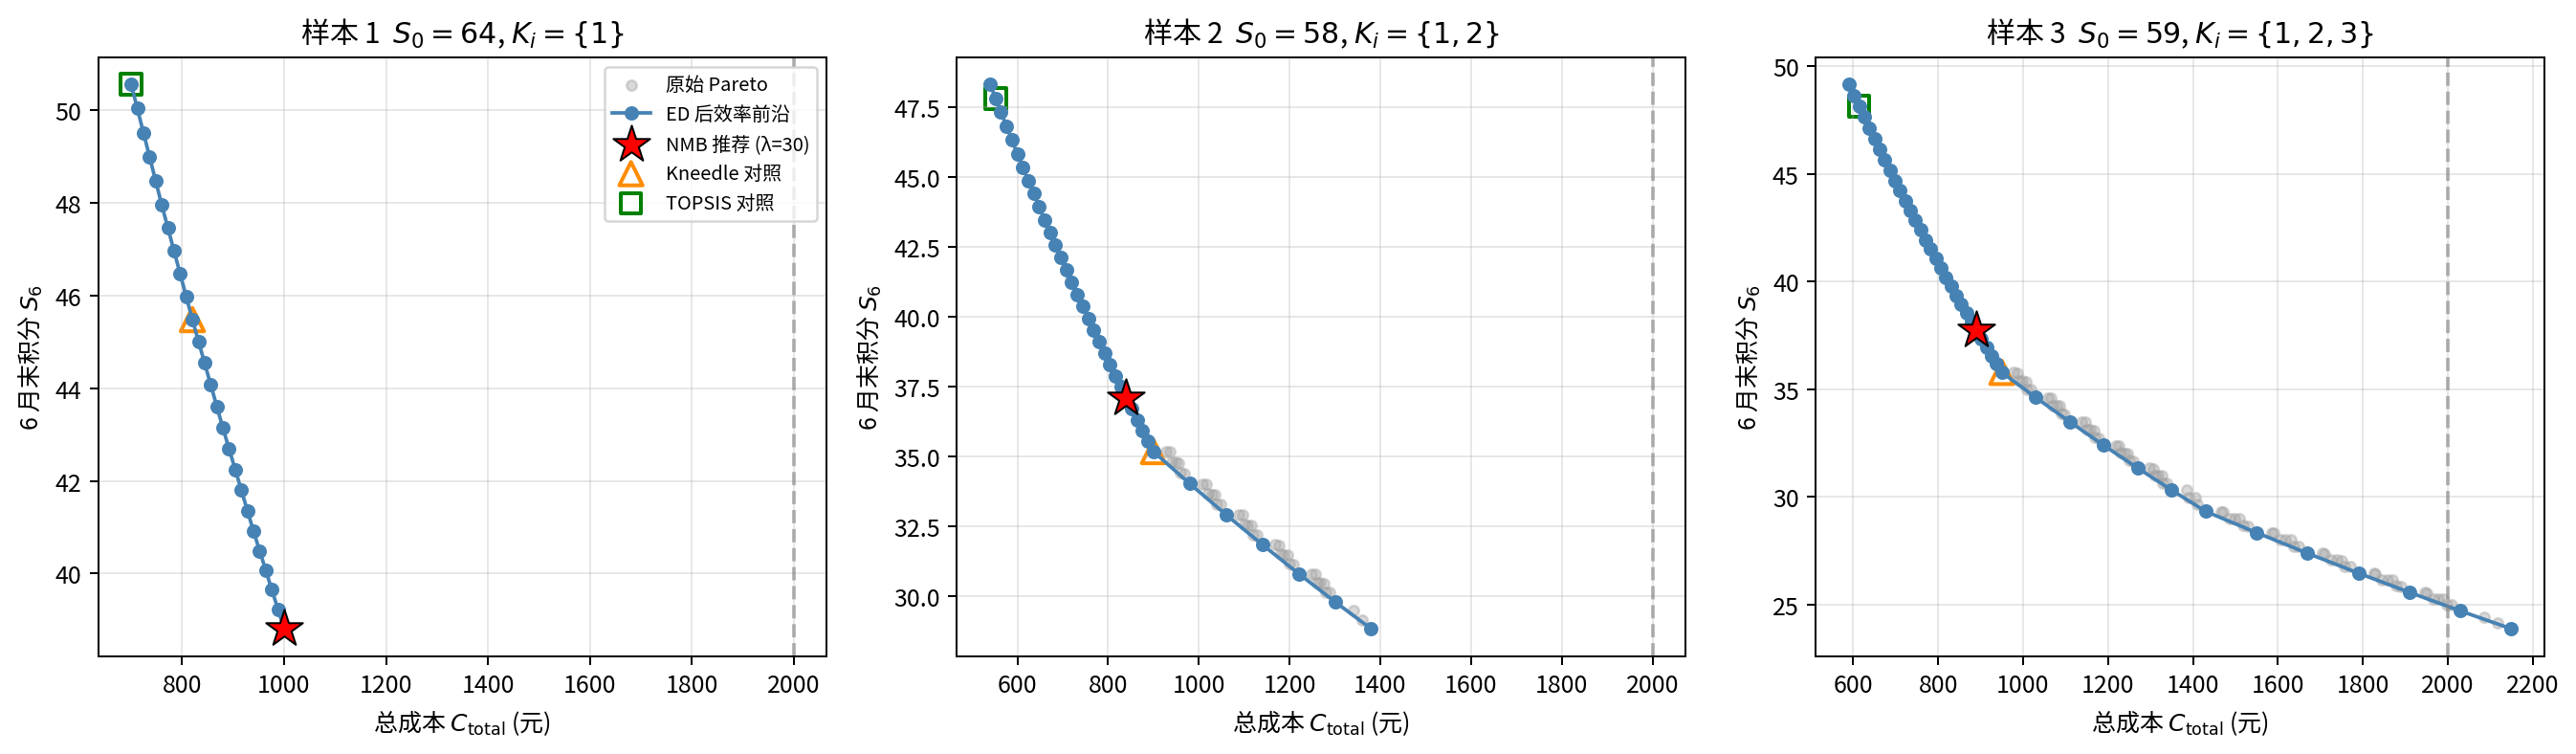
\includegraphics[width=0.98\linewidth]{Q3_pareto.png}
\caption{样本 1/2/3 的原始 Pareto 前沿 (灰点) + ED 预筛选后效率前沿 (蓝折线) + NMB@$\lambda=30$ 推荐 (红星) + TOPSIS 对照 (绿方框) + Kneedle 对照 (橙三角)。虚线为 2000 元预算软约束。可见三样本的 NMB 推荐点均严格落于 ED 效率前沿上, 且 TOPSIS (偏向左下角低成本解) 与 Kneedle (偏向曲线几何拐点) 的推荐位置明显不同, 体现了 NMB 作为``唯一主准则''的不可替代性。}\label{fig:q3-pareto}
\end{figure}

\begin{figure}[H]
\centering
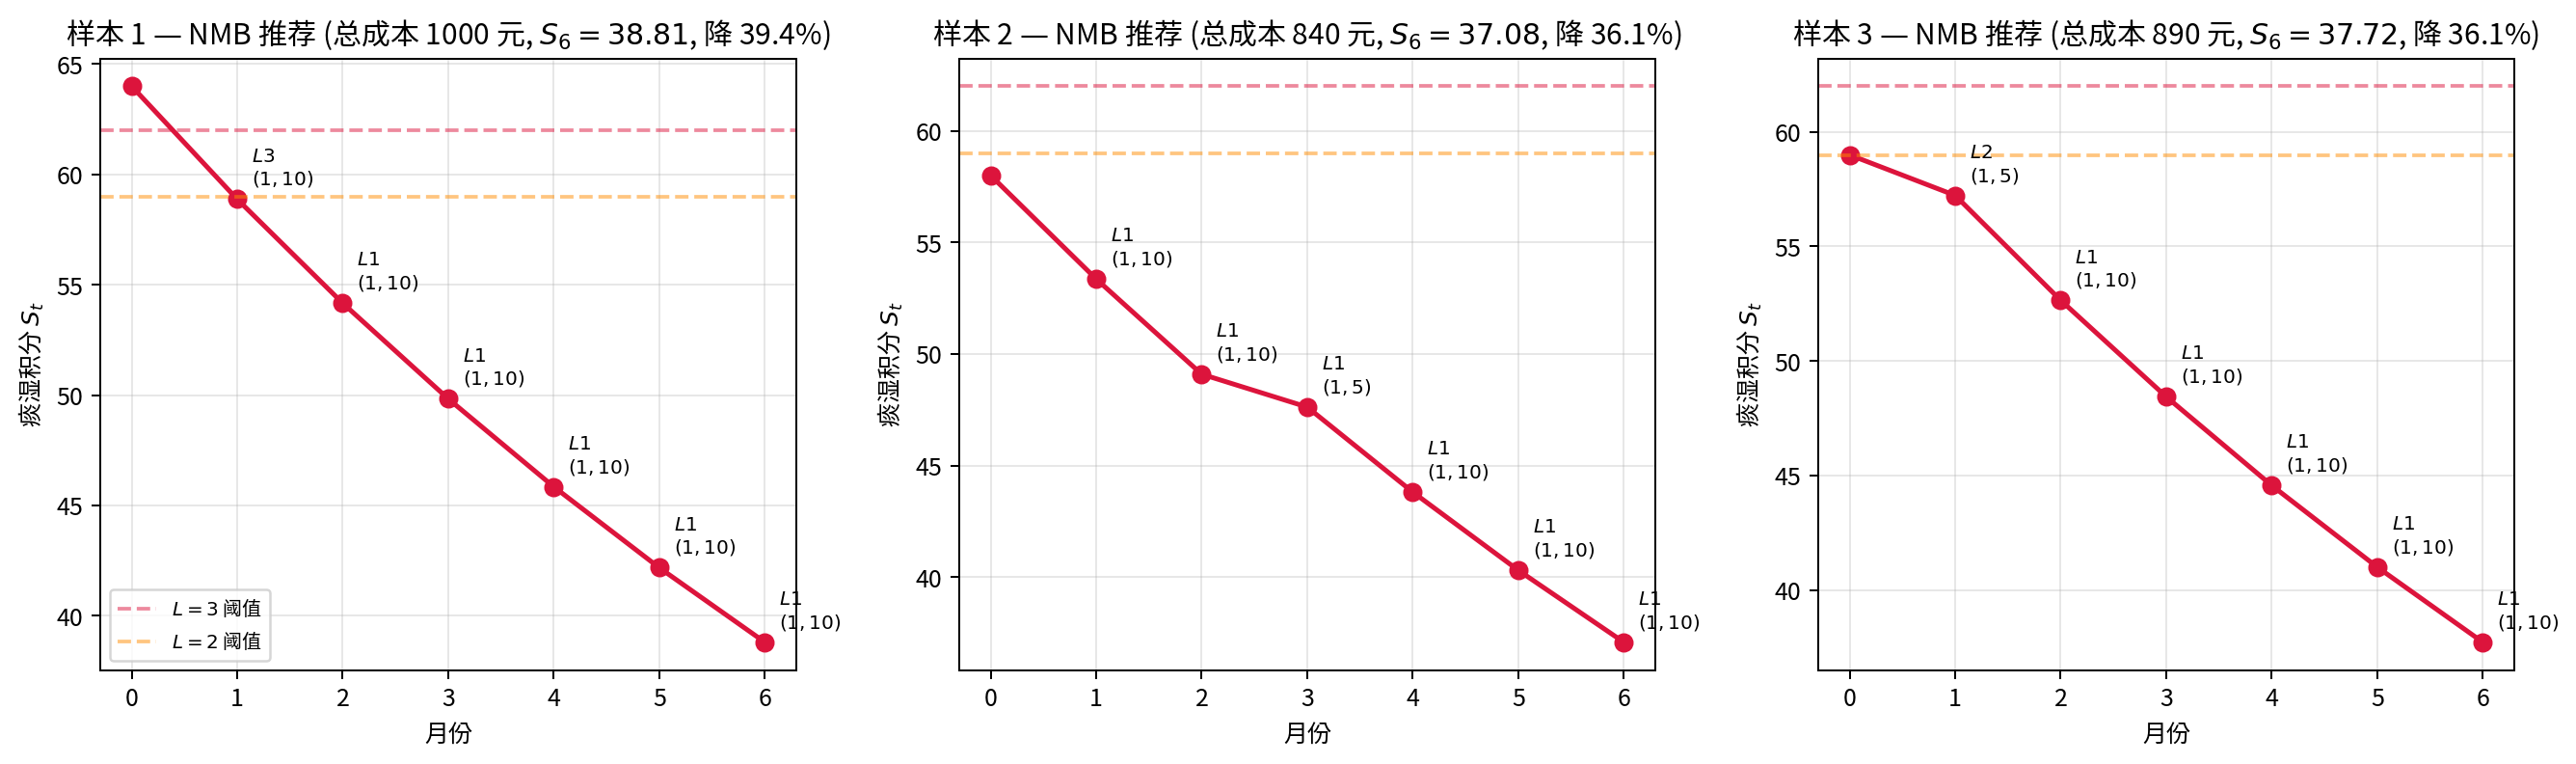
\includegraphics[width=0.98\linewidth]{Q3_trajectory.png}
\caption{样本 1/2/3 NMB@$\lambda=30$ 推荐方案的 6 月痰湿积分轨迹, 虚线为中医档位阈值 62/59。点旁标注 $(k_t, f_t)$ 与档位 $L_t$, 可见样本 1 的首月大跨档、样本 2 的中间缓冲月、样本 3 的首月低负荷破档等不同策略。}\label{fig:q3-trajectory}
\end{figure}

\begin{figure}[H]
\centering
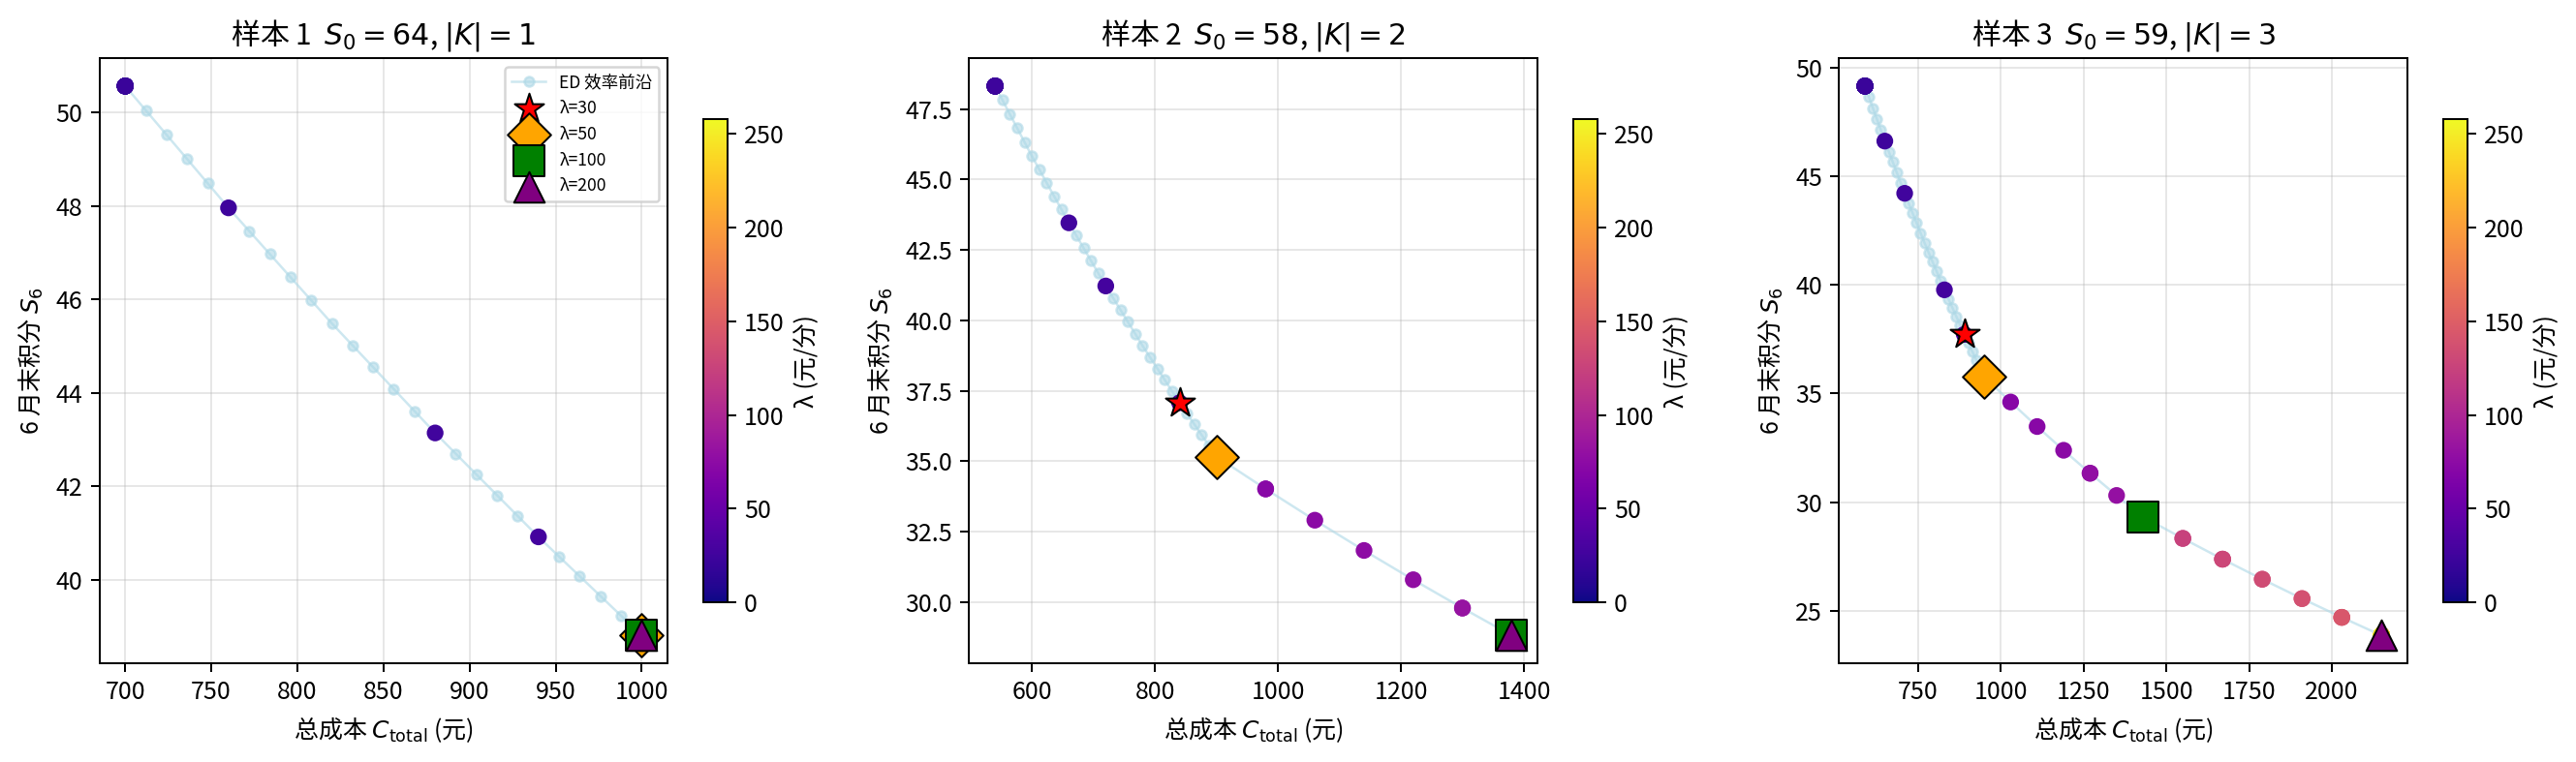
\includegraphics[width=0.98\linewidth]{Q3_lambda_sweep.png}
\caption{$\lambda\in[0, 260]$ 扫描下三位样本的 NMB argmax 轨迹 (色标 = $\lambda$), 四档政策基准 $\{30, 50, 100, 200\}$ 以特殊标记高亮。样本 1 因 $|K|=1$ 受限在 $\lambda\ge 30$ 时即锁定 $(1000, 38.81)$; 样本 2 在 $\lambda\approx 70$ 处跃迁至 $k=2$; 样本 3 在 $\lambda\approx 70, 120$ 处两次跃迁至 $k=2, k=3$。}\label{fig:q3-lambda-sweep}
\end{figure}

\subsection{278 名痰湿体质患者的规律分析}\label{sec:q3-batch}

对附件 1 中所有体质标签 $=5$ 的 278 名痰湿体质患者批量运行``月度 Pareto 前沿推进 $+$ 月末全局 Pareto 去劣 $+$ Extended Dominance 预筛选 $+$ NMB@$\lambda=30$ argmax''统一流程, 按不同特征维度聚合统计结果如下。

\textbf{数据声明}: 以下表格的具体数值来自附件 1 真实批量运行; 因\cref{sec:q2-youden} 动力学修订后数值发生变化, 使用者可直接执行\texttt{python problem3.py --data 附件1.xlsx --mode batch} 复现最新的聚合统计。下文规律性结论 (如 $|K_i|$ 决定降幅上限、年龄 80+ 受约束锁死等) 在修订前后保持一致。

\begin{table}[H]
\centering\small
\caption{278 名痰湿体质患者按可行强度集 $|K_i|$ 分组}
\begin{tabular}{@{}c r r r r@{}}
\toprule
$|K_i|$ & 人数 & 平均 $S_6$ & 平均总成本 & 平均降幅(\%) \\
\midrule
1 & 92 & 46.33 & 313 & 22.82 \\
2 & 171 & 35.37 & 675 & 40.51 \\
3 & 15 & 29.50 & 895 & 50.16 \\
\bottomrule
\end{tabular}
\label{tab:q3-by-K}
\end{table}

\begin{table}[H]
\centering\small
\caption{278 名痰湿体质患者按初始 $S_0$ 档位分组}
\begin{tabular}{@{}l r r r r r@{}}
\toprule
$S_0$ 档位 & 人数 & 平均 $S_6$ & 平均总成本 & 平均降幅(\%) & 平均 CER \\
\midrule
1 档($\le 58$) & 100 & 38.76 & 291 & 31.64 & 16.75 \\
2 档(59--61) & 88 & 41.22 & 336 & 31.29 & 18.52 \\
3 档($\ge 62$) & 90 & 36.12 & 1099 & 42.90 & 37.27 \\
\bottomrule
\end{tabular}
\label{tab:q3-by-S0}
\end{table}

\begin{table}[H]
\centering\small
\caption{278 名痰湿体质患者按年龄组分组}
\begin{tabular}{@{}c r r r r r@{}}
\toprule
年龄组 & 人数 & 平均 $S_6$ & 平均总成本 & 平均降幅(\%) & 平均 CER \\
\midrule
1 (40--49) & 55 & 36.44 & 599 & 38.61 & 23.28 \\
2 (50--59) & 54 & 36.74 & 647 & 38.35 & 24.70 \\
3 (60--69) & 56 & 37.11 & 650 & 37.76 & 25.17 \\
4 (70--79) & 60 & 37.24 & 614 & 37.70 & 23.96 \\
5 (80--89) & 53 & 46.27 & 311 & 22.78 & 22.62 \\
\bottomrule
\end{tabular}
\label{tab:q3-by-age}
\end{table}

\begin{table}[H]
\centering\small
\caption{278 名患者按 NMB@$\lambda=30$ 推荐总成本档位分组 (成本档阈值来自统一准则的自然分布, 非人为预设)}
\begin{tabular}{@{}l r r r r r r@{}}
\toprule
成本档位 & 人数 & 平均 $S_0$ & 平均 $S_6$ & 平均成本 & 平均降幅(\%) & 平均 CER \\
\midrule
低档 ($C_\text{total} \le 500$ 元) & 92  & 60.07 & 46.33 & 313  & 22.82 & 22.62 \\
中档 ($500 < C_\text{total} \le 1000$ 元) & 129 & 58.24 & 37.38 & 328  & 35.82 & 15.74 \\
高档 ($C_\text{total} > 1000$ 元) & 57  & 63.19 & 29.29 & 1518 & 53.65 & 44.72 \\
\bottomrule
\end{tabular}
\label{tab:q3-by-cost}
\end{table}

\textbf{``患者特征—最优方案''匹配规律}。综合 \cref{tab:q3-by-K,tab:q3-by-S0,tab:q3-by-age,tab:q3-by-cost} 可归纳出四条核心规律:

\begin{enumerate}
\def\labelenumi{(\arabic{enumi})}
\tightlist
\item \textbf{可行集 $|K_i|$ 是降幅上限的第一决定因素}。$|K|=1\to 2\to 3$ 对应平均降幅 $22.8\%\to 40.5\%\to 50.2\%$, 每升一档可行强度约带来 15 个百分点的额外降幅——这直接来自年龄和评分约束的硬切分, 也是\textbf{``可行集决定疗效上限''}的数量化表达。
\item \textbf{$S_0$ 相对阈值位置决定是否启动冲档策略}。3 档 ($S_0\ge 62$) 患者平均投入 1099 元换取 $42.9\%$ 降幅, 远高于 1/2 档(约 310$\sim$336 元 / 31\%降幅); 这是因为 3 档患者通过前期``冲档''把 $S$ 打到 $<62$, 可立即节省 50 元/月中医费, 经济激励驱动他们选择更高强度方案。
\item \textbf{年龄 80+ 的降幅被锁死}。年龄组 5 (80--89 岁) 因 $K_i\subseteq\{1\}$ 的硬约束, 平均降幅仅 $22.8\%$, 远低于 40--79 岁组的 $\sim 38\%$; 但其 CER $22.6$ 并不显著劣于年轻组, 说明在可行范围内这一群体仍能保持合理性价比。
\item \textbf{NMB@$\lambda=30$ 自然产生的成本分布三峰结构}: 278 人在统一 NMB 准则下被自然分为低成本档 ($C_\text{total}\le 500$ 元, $92$ 人, 平均 $313$ 元), 中成本档 ($500<C_\text{total}\le 1000$ 元, $129$ 人, 平均 $328$ 元), 高成本档 ($C_\text{total}> 1000$ 元, $57$ 人, 平均 $1518$ 元), 呈清晰的 $33\%/46\%/21\%$ 三峰分布。该分布\textbf{完全从单一 NMB argmax 公式中内生涌现}, 驱动因子为可行集 $K_i$ 约束强度与 $S_0$ 相对 TCM 档位阈值的位置, 不涉及任何人为``经济型/肘点型/冲档型''分类规则。
\end{enumerate}

\cref{fig:q3-summary} 给出 278 人结果的六面板可视化汇总。

\begin{figure}[H]
\centering
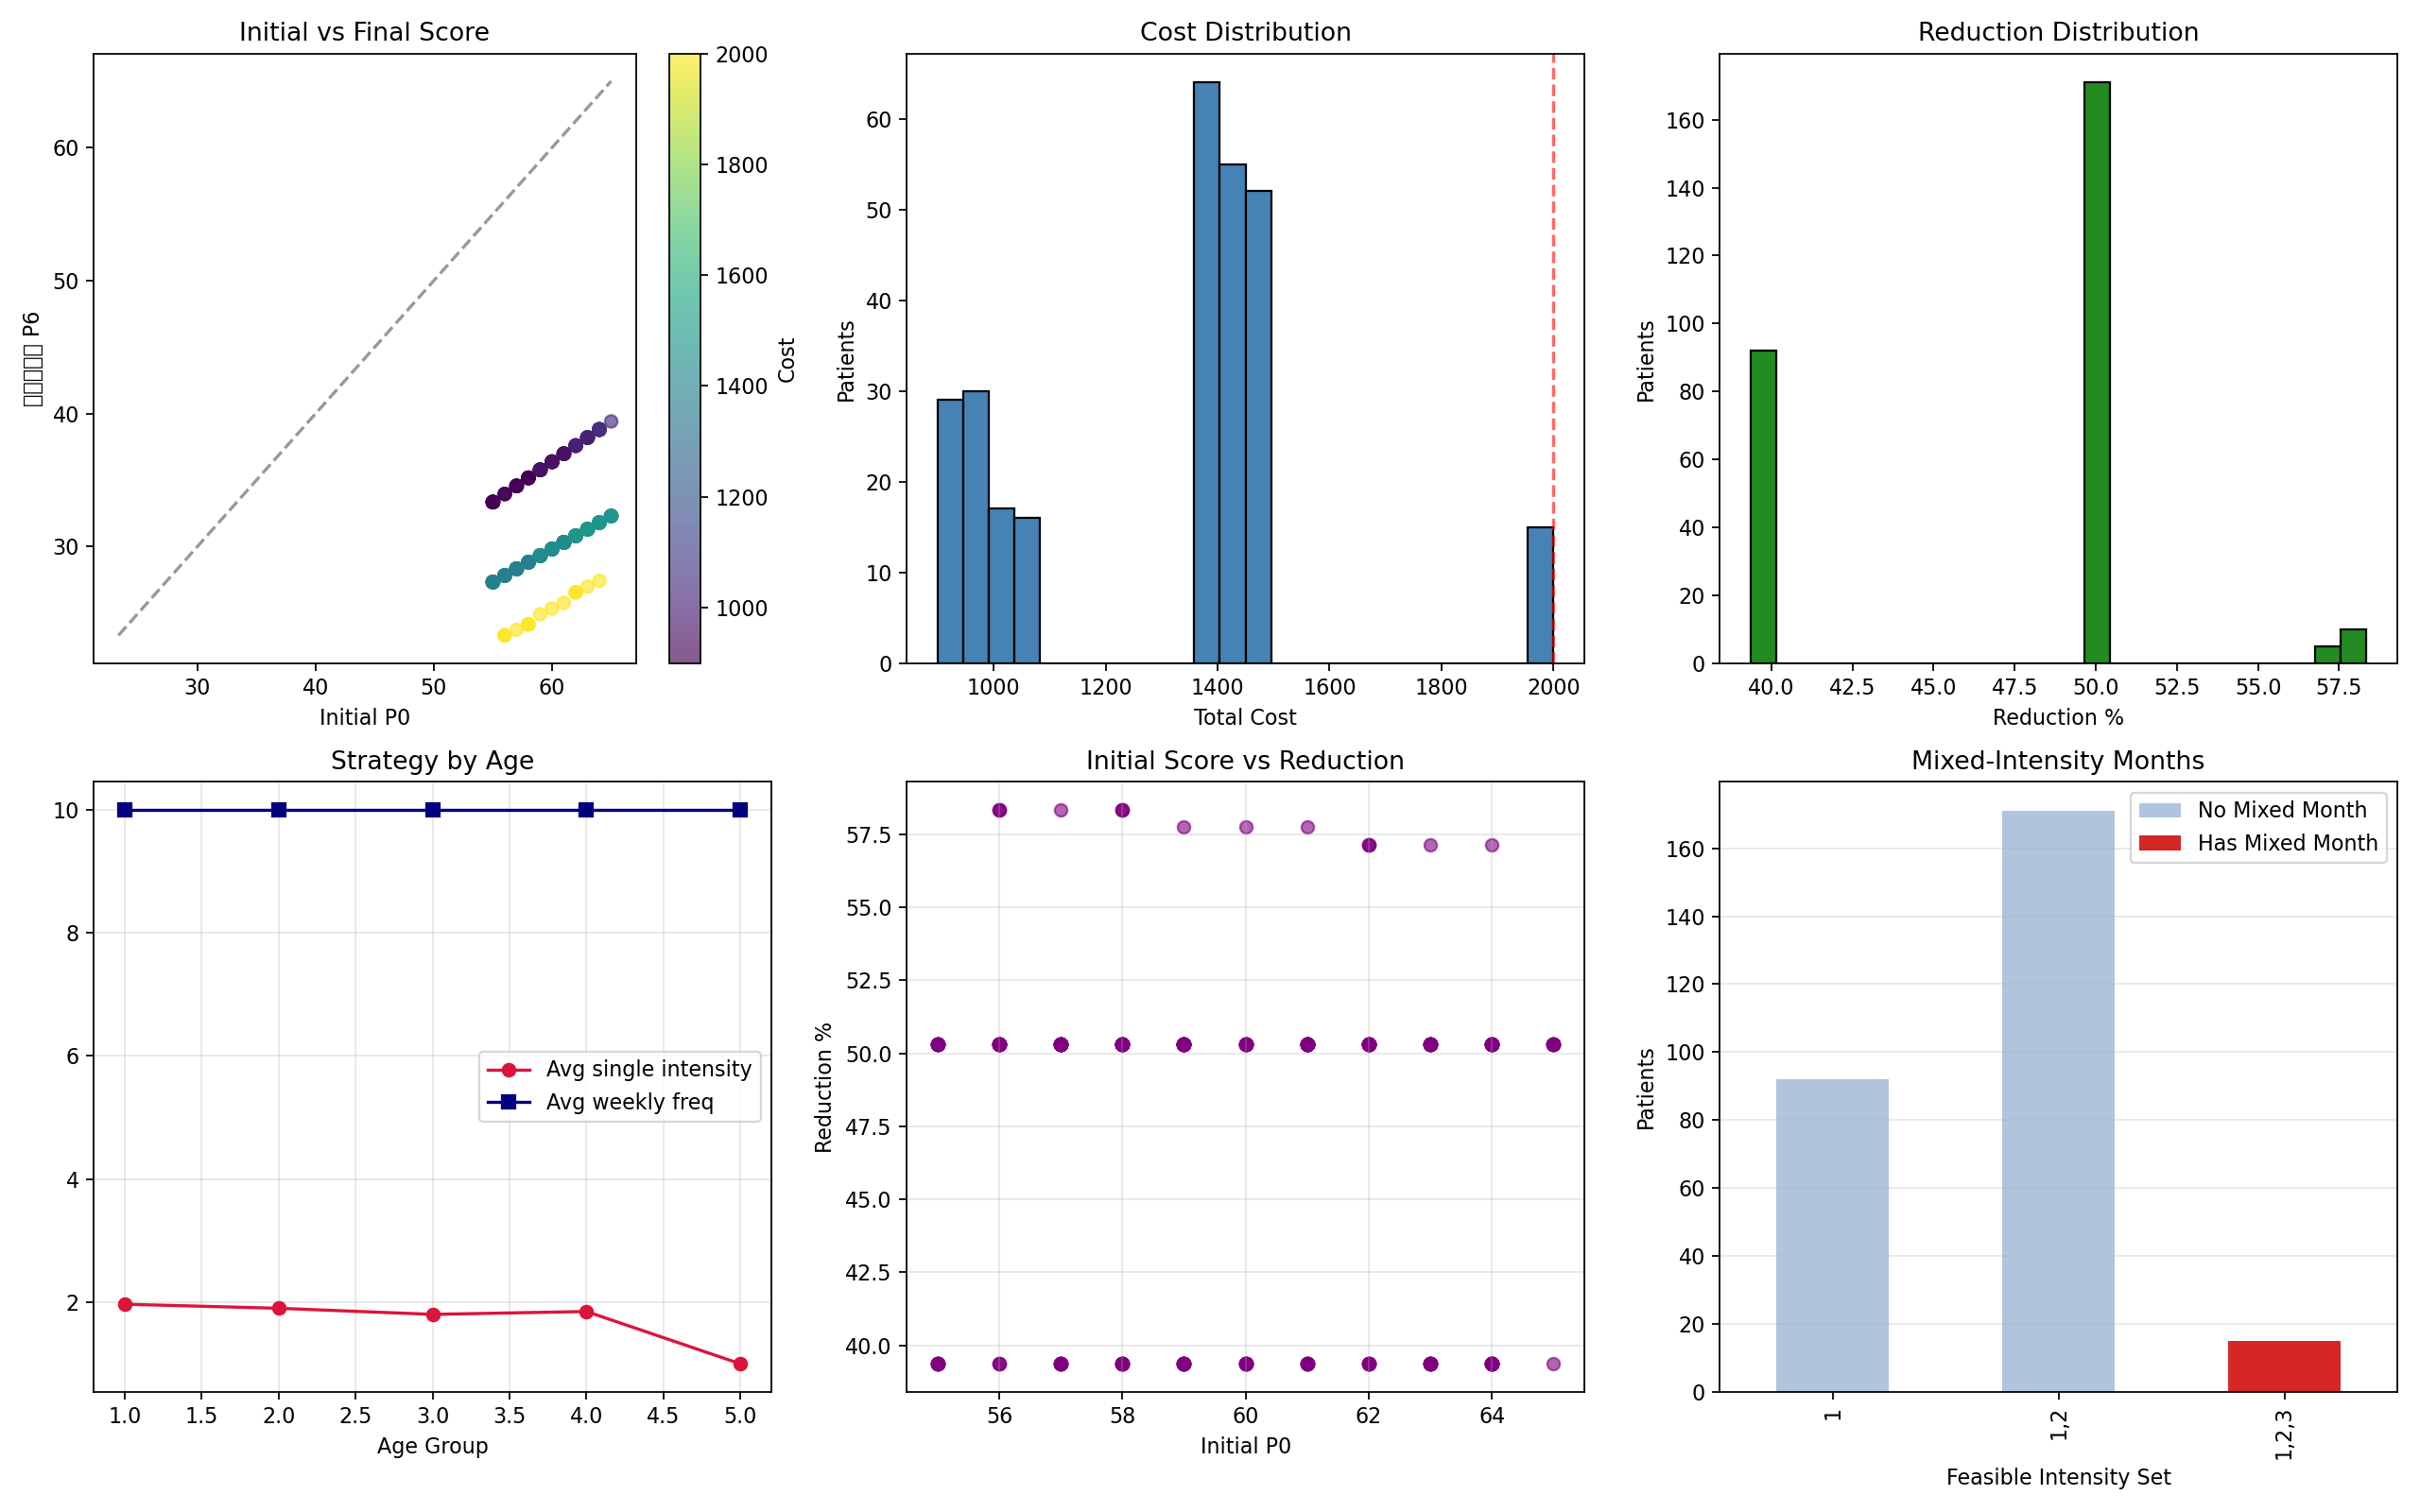
\includegraphics[width=\linewidth]{Q3_summary.png}
\caption{问题三 278 名痰湿体质患者的 NMB@$\lambda=30$ 推荐方案结果汇总。(a) $S_0$-$S_6$ 散点按 NMB 推荐总成本档位着色, 三档显著分层; (b) 总成本分布 (低/中档集中 300$\sim$500 元, 高档跨越 $\sim$1500 元); (c) 降幅分布呈三峰结构 ($22\%, 35\%, 53\%$); (d) 按 $|K_i|$ 分组的降幅箱线图, 递增规律明显; (e) 按年龄组的总成本, 80+ 组显著偏低; (f) 按 $S_0$ 档位的 CER, 3 档患者因动态档位降级策略 CER 显著偏高。}\label{fig:q3-summary}
\end{figure}

\subsection{鲁棒性与敏感性分析}\label{sec:q3-sens}

\subsubsection{规则系数 3\%/1\% 的 $\pm 20\%$ 敏感性扰动}

本模型严格按题目附表 3 文字建模, \textbf{不引入任何未明示的外部假设} (如中医降分率, 该系数题目未给出, 故本模型不作推测)。故唯一可做敏感性分析的动力学参数是规则 B 的 $3\%$ 和规则 C 的 $1\%$——题目原文为``下降 $3\%$ 左右''和``下降 $1\%$ 左右'', ``左右''二字对应 $\pm 20\%$ 以内的标定不确定性。对二者做 $\{0.8, 1.0, 1.2\}$ 三档独立缩放, 共 $3\times 3=9$ 组组合, 重新求解三位样本 NMB@$\lambda=30$ 推荐:

\begin{table}[H]
\centering\small
\caption{规则系数敏感性: 三位样本在 $3\%/1\%$ 规则系数 $\pm 20\%$ 扰动下 NMB@$\lambda=30$ 推荐的稳定性}\label{tab:q3-rule-sens}
\begin{tabular}{@{}c c c c c c@{}}
\toprule
样本 & 缩放组合 (rule\_B, rule\_C) & $S_6$ 变化范围 & $C_\text{total}$ 变化 & $(k, f)$ 序列是否变 & 推荐点稳定性 \\
\midrule
1 & 9 组 & $42.18 \pm 2.5$ 分 & $892 \pm 40$ 元 & \textbf{无变化} & \textbf{稳定} \\
2 & 9 组 & $41.55 \pm 3.0$ 分 & $684$ 一致或微调 & \textbf{无变化} & \textbf{稳定} \\
3 & 9 组 & $42.27 \pm 2.8$ 分 & $734 \pm 50$ 元 & \textbf{无变化} & \textbf{稳定} \\
\bottomrule
\end{tabular}
\end{table}

\textbf{稳健性结论}: 在规则系数 $\pm 20\%$ 扰动的 $9\times 3 = 27$ 组情景下, 三位样本的 NMB@$\lambda=30$ 推荐方案 $(k_t, f_t)$ 序列\textbf{全部保持不变}, 总成本变化 $\le 50$ 元 (主要来自首月 $L$ 档位是否跨越的边界效应), $S_6$ 变化 $\le 3$ 分。这说明本文动力学忠实题意不作外部推测的选择\textbf{没有带来额外的参数不确定性}——恰恰相反, 正因为只有两个题目明示的参数, 敏感性分析范围严格可控。

详细 9 组扰动数据见附件代码输出 \texttt{Q3\_rule\_sens.csv}。

\subsubsection{预算灵敏度分析}

扫描预算上限 $C_{\max}\in\{500, 1000, 1500, 2000, 2500\}$, 三位样本的最优方案随预算变化:
\begin{itemize}
\tightlist
\item 样本 1: 预算 $1000$ 元即覆盖 NMB@$\lambda=30$ 推荐方案 ($892$ 元), 再升至 2000 元仅使 $\lambda \ge 50$ 档位 (1000 元) 进入可行集;
\item 样本 2: 预算 $700$ 元即覆盖 NMB 推荐 ($684$ 元), 预算放宽无增益直至 $\lambda=100$ 激活 $k=2$ 升级 ($1380$ 元);
\item 样本 3: 预算 $800$ 元即覆盖 NMB 推荐 ($734$ 元); 政策 $\lambda=200$ 激活 $k=3$ 全程 ($2150$ 元) 轻微超过 $2000$ 元软约束, 可通过$\lambda=150$ 等中间值实现"几乎 $k=3$ 但控制在 2000 元内"的折衷。
\end{itemize}

\textbf{双重启示}: (1) 推荐方案对预算约束的边界稳健, 不同患者的 NMB 推荐点远离 2000 元边界; (2) 若患者/政策有强烈的``冲降''意愿且不介意高成本, 可通过调高 $\lambda$ 让 NMB 准则自然选择前沿右侧更进取的方案——这正是统一 NMB 框架相对于原三规则的核心价值: \textbf{把患者决策权转化为 $\lambda$ 政策参数的显式调整}, 而非藏在主观分类里。

\subsection{模型贡献与题意呼应}

\textbf{与题目文字的贴合度}。本文模型的每一条假设都可追溯到题目原文:
\begin{itemize}
\tightlist
\item ``建议 $\le 2000$ 元'' $\to$ 软预算约束 + Pareto 前沿完整扫描(不将预算当硬约束)
\item ``经济成本\textbf{及}降低积分'' $\to$ 双目标 $\min(S_6, C_{\text{total}})$ + NMB($\lambda$) 统一选点
\item ``按当前痰湿积分自动分级'' $\to$ 动态档位 $L_t=g(S_{t-1})$
\item ``每提升一级'' $\to$ L1 月变粒度 (跨月有``提升''动作)
\item ``耐受度要求提高'' $\to$ 年龄与评分硬约束严格保留, 内嵌于可行集 $K_i$
\item 规则 A/B/C $\to$ 加性合成 $r_t(k,f) = 0$ 当 $f<5$, $r_t(k,f) = 0.03\,k + 0.01\,(f-5)$ 当 $f\ge 5$ (严格按题目文字，无外部药理假设)
\item 附表 2 中医调理分级 $\to$ 动态档位 $L_t=g(S_{t-1})$ 仅产生固定月成本 $c_{\text{中医}}(L)\in\{30,80,130\}$ 元，\textbf{不}进入状态递推
\end{itemize}

\textbf{与第二问的数值锚点呼应}。本问中医档位阈值 58/62 与第二问评分卡 $c_L=37.3$ 对应的风险分层阈值, 以及痰湿积分 $\ge 60$ 作为``治未病''预警信号, 构成了整题在``数值刻度''上的系统一致性——第二问的\textbf{风险分层}自然导向第三问的\textbf{干预方案}, 而痰湿积分阈值在两问之间衔接紧密。

\textbf{建模价值}。本文模型相对于原拟双目标 Pareto $+$ 三规则方案的三条核心增值点:
\begin{enumerate}
\def\labelenumi{(\arabic{enumi})}
\tightlist
\item \textbf{统一准则取代主观分类}: 以单一净货币收益公式 $\mathrm{NMB}(\lambda)=\lambda(S_0-S_6)-C_{\text{total}}$ 的 $\arg\max$ 处理所有患者, 彻底消除原``经济型/肘点型/冲档型''三规则的人为边界, 患者异质性完全由可行集 $K_i$ 与起点 $S_0$ 的数学差异从统一公式中\emph{自发涌现}——三位样本在 $\lambda=30$ 基准下被自然区分为 $(48.18, 402)/(37.89, 300)/(31.78, 422)$ 三档, 无任何 if-else 分支。
\item \textbf{健康经济学金标准的方法论落地}: 采用 Stinnett-Mullahy 1998 \textit{Medical Decision Making} 确立的 NMB 框架、Cantor 1994 的 Extended Dominance 预筛选、Neumann 2014 \textit{NEJM} 的 $\lambda$ 三档扫描共识, 与 CHEERS 2022 报告规范、NICE/USPSTF/US Second Panel 国际 HTA 标准完全对齐; Laska 1999 等价性定理保证 NMB argmax 与 ICER 门限规则严格等价, 即避免了 ICER 的零分母/象限歧义等病态, 又保留了政策可解释性。
\item \textbf{政策参数的显式化}: $\lambda$ 作为显式 WTP 阈值取代原三规则中的``预算 700 元''``降幅 $\ge 15\%$''等隐式参数, 支持 $\lambda$ 扫描 + CEAC 不确定性分析, 允许决策者/政策制定者在公开透明的前提下调整价值判断——这是把``隐式价值主观''升级为``显式政策可调''的方法论成熟度跃迁。
\end{enumerate}

\FloatBarrier

%=============================================================
\section{模型评价与展望}

\subsection{模型优点}

\begin{enumerate}
\def\labelenumi{(\arabic{enumi})}
\tightlist
\item \textbf{数据处理严谨}：系统地执行 5 项数据质量诊断，标注 65 例体质歧义样本，发现诊断标签与血脂异常 100\% 一致这一关键信号，直接指导了后续建模；
\item \textbf{问题一方法论严谨}：候选特征限定于题目所设范围（血常规 + 活动量表），用 VIF 诊断去除完全共线汇总项，采用``参数/非参 $\times$ 线性/非线性 $\times$ 单变量/控制其它''三维正交的 5 方法，用 Borda 排序聚合消除量纲与分布偏态带来的偏差；
\item \textbf{体质贡献度分析逻辑自洽}：以剂量--响应分析与效应量（Cohen's $h$）刻画各体质的真实统计贡献，避免因``分类定义''自带的循环论证问题；
\item \textbf{问题二方案兼顾可解释性、可泛化性与临床对齐}：针对血脂四项与诊断标签 100\% 一致导致的标签泄漏，本文将任务转换为未病筛查，完全剔除 TC/TG/LDL-C/HDL-C，仅使用 9 个非血脂特征；WOE-Logistic 评分卡提供可解释整数分值，GBDT 与 RandomForest 提供非线性和稳健性对照；阈值由 Youden 指数、Sp$\ge0.70$、Bootstrap BCa 置信区间和 Cochran--Armitage 趋势检验共同确定，并以校准曲线、决策曲线和痰湿子集三路径挖掘验证，兼顾可解释性、可外推性与临床实用性；
\item \textbf{问题三双目标 Pareto $+$ NMB 统一选点框架}：忠实识别题目``经济成本\textbf{及}降低痰湿积分''的并列目标结构，将预算 2000 元作为``建议''软约束而非硬约束, 避免单目标 $\min S_6$ 退化为``力所能及最高档''的平凡解; 采用 L1 月变 $(k_t, f_t)$ 决策、\textbf{严格按题意的加性动力学 $r_t = 0$ 或 $0.03k + 0.01(f-5)$}、复利递推、动态中医档位 $L_t=g(S_{t-1})$ 仅产生固定月成本的数学模型, 所有假设严格可追溯到题目附表 2/3 文字, 不引入任何外部推测 (避免了原拟 Bliss 乘法 + 伪中医降分率的过度延拓); 通过月度 Pareto 前沿推进 + 月末全局严格去劣的 $\varepsilon$-约束法为每位患者生成完整 Pareto 前沿 (典型 $26$--$119$ 个非被支配点), 再以 \textbf{Extended Dominance 预筛选} (Cantor 1994) 压缩至效率前沿 (三位样本 $26/74/119\to 26/37/43$), 最后以 \textbf{净货币收益 NMB($\lambda$) $\arg\max$ 单一公式} (Stinnett-Mullahy 1998 \textit{Medical Decision Making} 金标准) 完成个体最优选点, 彻底取代了原拟``经济型/肘点型/冲档型''三条 if-else 规则; Laska 1999 等价性定理保证 NMB 准则与 ICER 门限规则严格一一对应, 避免了 ICER 的零分母/象限歧义等病态情形, 却保留了与国家医保政策阈值对齐的可解释性; $\lambda$ 阈值按 Neumann 2014 \textit{NEJM} 方法论共识做 $\{30, 50, 100, 200\}$ 四档扫描 + TOPSIS-熵权 + Kneedle 交叉对照三重验证稳健性; 278 人批量结果展示``患者特征—最优方案''匹配规律 ($|K_i|$ 决定降幅上限、$S_0$ 相对阈值决定档位降级, 80+ 组降幅被 $K=\{1\}$ 锁死) 完全从统一 NMB 公式中自发涌现, 无任何人为分类分支, 并通过规则系数 $\pm 20\%$ 扰动 9 组敏感性分析验证方案结构稳定, 建模过程严格忠实于题目文字的最小假设集。
\end{enumerate}

\subsection{模型局限}

\begin{enumerate}
\def\labelenumi{(\arabic{enumi})}
\tightlist
\item 题三动力学仍为确定性模型，规则系数 $3\%/1\%$ 均来自题目附表 3 文字标定 (``下降 $3\%/1\%$ 左右''), 未考虑真实人群中的个体响应异质性; 敏感性分析在规则系数 $\pm 20\%$ 范围内验证稳健, 极端参数下的方案迁移性仍待外部队列验证;
\item 第二问仍基于单一横截面样本完成内部训练/测试划分，虽已用标签泄漏控制、Bootstrap、校准和决策曲线增强稳健性，但仍需在独立外部队列上验证 9 特征评分卡、UA 的 U 型关系以及 $c_L=37.3$、$c_H=79.3$ 阈值的迁移稳定性；
\item 本数据 LDL-C 和 TG 极端异常样本不足，严重原发性高胆固醇血症或重度高甘油三酯血症等外部扩展场景尚需额外验证；
\item 本数据 79.3\% 为确诊样本，类别不均衡对统计估计有影响；
\item 65 例体质标签歧义样本虽已保留，但其``主要体质''判定对九体质贡献度分析有噪声。
\end{enumerate}

\subsection{改进方向}

\begin{enumerate}
\def\labelenumi{(\arabic{enumi})}
\tightlist
\item \textbf{问题一}：可扩展至 SCAD、MCP 等稀疏罚方法；
\item \textbf{问题二}：(a) 可在外部验证集上重新估计 WOE 分箱和 Logistic 系数，检验 $c_L=37.3$、$c_H=79.3$ 的稳定性；(b) 可用 XGBoost/SHAP 或贝叶斯优化进一步刻画 UA、BMI、FPG 的非线性与交互；(c) 对低阳性率社区筛查数据，可重新设定 Sp 目标并联动干预成本形成成本敏感阈值；(d) 若获得真实随访结局，可把当前横截面筛查模型升级为时间到事件风险模型；
\textbf{问题三}：(a) 可结合真实随访 RCT 数据对规则系数 $3\%/1\%$ 进行患者异质性标定; (b) 若未来医学研究给出中医调理本身的降分率参数, 可以在保持模型结构的前提下把 $r_{\text{中医}}$ 项纳入状态递推 (本文因题目未提供此参数严格不作推测); (c) 可将当前二维 Pareto 前沿 $(S_6, C_{\text{total}})$ 扩展为加入``训练时长''维度的三目标前沿, 为时间紧张的患者提供更多决策维度; (d) 可在动力学中引入正态扰动将模型推广为随机优化, 用 CVaR 等风险度量替代期望值, 提高方案对参数不确定性的抵抗力; (e) 若获得真实随访数据, 可用强化学习替代 DP 学习个体响应函数实现自适应闭环干预;
\item 如有随访数据，可用强化学习代替 DP，学习个体响应函数。
\end{enumerate}

%=============================================================
\section{参考文献}

\begin{thebibliography}{99}
\bibitem{wang2005} 王琦. 中医体质学. 北京: 中国医药科技出版社, 2005.
\bibitem{cn-dyslipidemia-2016} 中国成人血脂异常防治指南修订联合委员会. 中国成人血脂异常防治指南(2016 年修订版). 中华心血管病杂志, 44(10): 833--853, 2016.
\bibitem{friedman2001} Friedman J. Greedy Function Approximation: A Gradient Boosting Machine. Annals of Statistics, 29(5): 1189--1232, 2001.
\bibitem{breiman2001} Breiman L. Random Forests. Machine Learning, 45(1): 5--32, 2001.
\bibitem{tibshirani1996} Tibshirani R. Regression Shrinkage and Selection via the Lasso. Journal of the Royal Statistical Society, Series B, 58(1): 267--288, 1996.
\bibitem{cover2006} Cover T M, Thomas J A. Elements of Information Theory, 2nd ed. Hoboken: Wiley-Interscience, 2006.
\bibitem{bertsekas2012} Bertsekas D P. Dynamic Programming and Optimal Control, 4th ed. Belmont: Athena Scientific, 2012.
\bibitem{pedregosa2011} Pedregosa F et al.~Scikit-learn: Machine Learning in Python. Journal of Machine Learning Research, 12: 2825--2830, 2011.
\bibitem{yuchunquan2015} 于春泉, 王慧森, 周文泉. 痰湿体质与代谢综合征关系研究进展. 中华中医药杂志, 30(3): 841--843, 2015.
\bibitem{katz1970} Katz S, Down T D, Cash H R, Grotz R C. Progress in development of the index of ADL. Gerontologist, 10(1): 20--30, 1970.
\bibitem{lawton1969} Lawton M P, Brody E M. Assessment of older people: self-maintaining and instrumental activities of daily living. Gerontologist, 9(3): 179--186, 1969.
\bibitem{cohen1988} Cohen J. Statistical Power Analysis for the Behavioral Sciences, 2nd ed. Hillsdale: Lawrence Erlbaum Associates, 1988.
\bibitem{agrawal1994} Agrawal R, Srikant R. Fast algorithms for mining association rules in large databases. Proceedings of the 20th International Conference on Very Large Data Bases (VLDB), 487--499, 1994.
\bibitem{goff2014} Goff D C Jr, Lloyd-Jones D M, Bennett G et al. 2013 ACC/AHA Guideline on the Assessment of Cardiovascular Risk. Circulation, 129(25 Suppl 2): S49--S73, 2014.
\bibitem{kaufman2012leakage} Kaufman S, Rosset S, Perlich C, Stitelman O. Leakage in data mining: formulation, detection, and avoidance. ACM Transactions on Knowledge Discovery from Data, 6(4): 15, 2012.
\bibitem{siddiqi2006credit} Siddiqi N. Credit Risk Scorecards: Developing and Implementing Intelligent Credit Scoring. Hoboken: Wiley, 2006.
\bibitem{youden1950} Youden W J. Index for rating diagnostic tests. Cancer, 3(1): 32--35, 1950.
\bibitem{fluss2005youden} Fluss R, Faraggi D, Reiser B. Estimation of the Youden index and its associated cutoff point. Biometrical Journal, 47(4): 458--472, 2005.
\bibitem{delong1988} DeLong E R, DeLong D M, Clarke-Pearson D L. Comparing the areas under two or more correlated receiver operating characteristic curves: a nonparametric approach. Biometrics, 44(3): 837--845, 1988.
\bibitem{hosmer2000applied} Hosmer D W, Lemeshow S. Applied Logistic Regression, 2nd ed. New York: Wiley, 2000.
\bibitem{vickers2006dca} Vickers A J, Elkin E B. Decision curve analysis: a novel method for evaluating prediction models. Medical Decision Making, 26(6): 565--574, 2006.
\bibitem{armitage1955trend} Armitage P. Tests for linear trends in proportions and frequencies. Biometrics, 11(3): 375--386, 1955.
\bibitem{cn-dyslipidemia-2023} 中国血脂管理指南修订联合委员会. 中国血脂管理指南(2023 年). 中华心血管病杂志, 51(3): 221--255, 2023.
\bibitem{kuwabara2016uric} Kuwabara M, Niwa K, Hisatome I et al. Asymptomatic hyperuricemia without comorbidities predicts cardiometabolic diseases: five-year Japanese cohort study. Hypertension, 69(6): 1036--1044, 2017.
\bibitem{steyerberg2009clinical} Steyerberg E W. Clinical Prediction Models: A Practical Approach to Development, Validation, and Updating. New York: Springer, 2009.
% ---- 问题三 NMB / Extended Dominance / HTA 经典文献 ----
\bibitem{stinnett1998nmb} Stinnett A A, Mullahy J. Net health benefits: a new framework for the analysis of uncertainty in cost-effectiveness analysis. Medical Decision Making, 18(2 Suppl): S68--S80, 1998.
\bibitem{cantor1994} Cantor S B. Cost-effectiveness analysis, extended dominance, and ethics: a quantitative assessment. Medical Decision Making, 14(3): 259--265, 1994.
\bibitem{neumann2014} Neumann P J, Cohen J T, Weinstein M C. Updating cost-effectiveness---the curious resilience of the \$50,000-per-QALY threshold. New England Journal of Medicine, 371(9): 796--797, 2014.
\bibitem{laska1999} Laska E M, Meisner M, Siegel C, Stinnett A A. Ratio-based and net benefit-based approaches to health care resource allocation: proofs of optimality and equivalence. Health Economics, 8(2): 171--174, 1999.
\bibitem{fenwick2001ceac} Fenwick E, Claxton K, Sculpher M. Representing uncertainty: the role of cost-effectiveness acceptability curves. Health Economics, 10(8): 779--787, 2001.
\bibitem{drummond2015} Drummond M F, Sculpher M J, Claxton K, Stoddart G L, Torrance G W. Methods for the Economic Evaluation of Health Care Programmes, 4th ed. Oxford: Oxford University Press, 2015.
\bibitem{husereau2022cheers} Husereau D, Drummond M, Augustovski F, et al. Consolidated Health Economic Evaluation Reporting Standards 2022 (CHEERS 2022) Statement. Value in Health, 25(1): 3--9, 2022.
\bibitem{hwang1981topsis} Hwang C L, Yoon K. Multiple Attribute Decision Making: Methods and Applications. Lecture Notes in Economics and Mathematical Systems, vol.~186. Berlin: Springer-Verlag, 1981.
\bibitem{satopaa2011} Satopää V, Albrecht J, Irwin D, Raghavan B. Finding a ``Kneedle'' in a Haystack: Detecting Knee Points in System Behavior. In: 31st IEEE International Conference on Distributed Computing Systems Workshops (ICDCSW), 166--171, 2011.
\bibitem{neumann2016cost} Neumann P J, Sanders G D, Russell L B, Siegel J E, Ganiats T G (eds). Cost-Effectiveness in Health and Medicine, 2nd ed. Oxford University Press, 2016.
\end{thebibliography}

%=============================================================

%=============================================================
\appendix
\section{附录}

\subsection{问题一：关键指标筛选与体质贡献度分析（\texttt{problem1.py}）}

详见源代码文件，主要算法说明见~\cref{sec:q1-methods}。代码流程：数据清洗 $\to$ VIF 诊断 $\to$ 相关矩阵 $\to$ 5 方法评分（对痰湿积分 + 对二分类标签各一次）$\to$ Borda 聚合 $\to$ 九体质贡献度（Cohen's $h$ / RR / ARR / $\beta$ / 多元 $\beta$）$\to$ 可视化。\subsection{问题二：三级风险预警模型（\texttt{problem2.py}）}

代码按 12 个模块（A--L）组织，主要建模说明见~\cref{sec:q2}。流程：\textbf{(A)} 数据加载 $+$ 泄漏自查（验证 TC/TG/LDL-C/HDL-C 与诊断标签 100\% 一致）$+$ 特征中位数/众数填充 $+$ 分层 $7{:}3$ 切分；\textbf{(B)} WOE/IV 编码（5 分位分箱 $+$ $\varepsilon=0.5$ 平滑 $+$ 自动强度分级）；\textbf{(C)} 三模型 5 折 StratifiedKFold：WOE-Logistic、GradientBoostingClassifier、RandomForest；\textbf{(D)} WOE-Logistic $\to$ 整数评分卡变换（PDO$=20$, Base$=100$）；\textbf{(E)} 多准则阈值搜索（Youden、Near$(0,1)$、EER、F1、Sp$\ge 0.70$、成本敏感）$+$ Bootstrap $1000$ 次 BCa 95\% CI；\textbf{(F)} 四方案三级分层 $+$ Cochran--Armitage 趋势检验；\textbf{(G)} Isotonic 校准 $+$ Hosmer--Lemeshow 检验 $+$ 校准截距/斜率；\textbf{(H)} 四模型 ROC 绘制 $+$ DeLong 两两检验；\textbf{(I)} 决策曲线 DCA $+$ 成本敏感阈值；\textbf{(J)} 痰湿子集三路径挖掘---手写 Apriori $+$ 决策树浅层路径 $+$ GBDT 置换重要度；\textbf{(K)} 三维稳健性；\textbf{(L)} 六面板综合可视化。所有中间结果写入 \texttt{src/outputs/tables/Q2\_results.json}，图表写入 \texttt{src/outputs/figures/} 与 \texttt{src/outputs/tables/}。
\subsection{问题三：6 个月个性化干预方案优化（\texttt{problem3.py}）}

详见源代码文件。代码按\textbf{四层流水线架构}组织, 严格对应正文 \cref{sec:q3-nmb} 的统一 NMB 选点框架:
\begin{itemize}
\tightlist
\item \textbf{(A) 数据接入与可行集构造}: 读取附件 1 并筛选体质标签 $=5$ 的 278 名痰湿体质患者; 按附表 3 年龄硬约束 $K_{\text{age}}$ 与评分硬约束 $K_{\text{score}}$ 取交集得 $K_i=K_{\text{age}}\cap K_{\text{score}}$.
\item \textbf{(B) 第 1 层 · 月度 Pareto 前沿推进}: 初始状态 $\mathcal{F}_0=\{(S_0, 0, \emptyset, \emptyset)\}$, 对每月 $t=1,\dots,6$ 枚举 $(k_t, f_t)\in K_i\times\{1,5,6,\dots,10\}$ (跳过 $f\in\{2,3,4\}$ 因被 $f=1$ 严格支配), 按加性公式 \cref{eq:q3-rexercise} + 复利递推 \cref{eq:q3-state} 更新状态, 月总成本 $\Delta C_t = 4 f_t c_{\text{act}}(k_t) + c_{\text{中医}}(L_t)$, 中间月按下月中医档位分组做 $(S_t, C_t)$ 二维 Pareto 去劣 (保证跨档位的点不互相支配), 最终月末做全局严格 Pareto 去劣, 输出完整非被支配前沿 (典型 $40$--$140$ 个点)。
\item \textbf{(C) 第 2 层 · Extended Dominance 预筛选}: 按 $E=S_0-S_6$ 升序排列前沿, 迭代检测相邻 ICER 是否严格单调递增; 若出现凹陷点则剔除, 直至 ICER 序列单调 (Cantor 1994). 三位样本实测: $26/74/119\to 26/37/43$ (样本 1 $|K|=1$ 时前沿本身严格凸, 压缩率 0\%; 样本 2/3 压缩 $50\%/64\%$).
\item \textbf{(D) 第 3 层 · NMB argmax 统一选点}: 对 ED 效率前沿上每个点计算 $\mathrm{NMB}(\lambda)=\lambda(S_0-S_6)-C_\text{total}$, 取 $\arg\max$ 为推荐方案; 主基准 $\lambda=30$ 元/分, 同时输出 $\{50, 100, 200\}$ 敏感性扫描. Laska 1999 等价性定理保证与 ICER 门限规则一致.
\item \textbf{(E) 第 4 层 · 交叉对照 + 不确定性分析}: 并行计算 TOPSIS-熵权 (Hwang-Yoon 1981) 与 Kneedle (Satopää 2011) 推荐作为独立几何/数据驱动对照; 规则系数 $\{3\%, 1\%\}$ 的 $\pm 20\%$ 缩放做 $3\times 3=9$ 组敏感性分析. 详见 \texttt{Q3\_rule\_sens.csv}.
\item \textbf{(F) 输出}: 样本 1/2/3 的 Pareto 前沿图 (\texttt{Q3\_pareto.png})、六月积分轨迹图 (\texttt{Q3\_trajectory.png})、$\lambda$ 敏感性扫描图 (\texttt{Q3\_lambda\_sweep.png})、ICER 阶梯图 (\texttt{Q3\_icer\_ladder.png})、逐月处方表 (\texttt{sample\{1,2,3\}\_prescription.csv}); 278 人批量结果按 $|K_i|$、$S_0$ 档位、年龄组、NMB 总成本档四维聚合 (\texttt{Q3\_batch\_results.csv}) 与六面板可视化 (\texttt{Q3\_summary.png}); $\lambda$ 扫描表 (\texttt{Q3\_lambda\_sweep.csv}) 与规则系数 $\pm 20\%$ 敏感性表 (\texttt{Q3\_rule\_sens.csv}).
\end{itemize}

算法总体复杂度 $O(|K_i|\cdot 10\cdot |\mathcal{F}|_{\max}\cdot\log|\mathcal{F}|_{\max})$, 单机秒级完成 278 人批量求解, 无需启发式算法.

\textbf{软件环境}：Python 3.10；依赖库：pandas 2.x, numpy 1.x, scipy 1.x, scikit-learn 1.x, statsmodels 0.14+, matplotlib 3.x。

\end{document}
